%\documentclass[handout]{beamer}
%\usepackage{pgfpages}
%\pgfpagesuselayout{4 on 1}[a4paper,border shrink=5mm,landscape]
\documentclass{beamer}
\usetheme{Boadilla}%Madrid}%Warsaw}
%\usecolortheme{dolphin}
%\useinnertheme{rectangles}
%\useoutertheme{tree}
%\usefonttheme{serif}

\usepackage[utf8]{inputenc}
\usepackage[english]{babel}
%\usepackage[brazil]{babel}   
\usepackage{listings}
\usepackage{booktabs}
\usepackage{xcolor}
\usepackage{hyperref}

\definecolor{codegreen}{rgb}{0,0.6,0}
\definecolor{codegray}{rgb}{0.3,0.3,0.3}
\definecolor{codepurple}{rgb}{0.58,0,0.82}
\definecolor{backcolour}{rgb}{0.95,0.95,0.92}

\lstdefinestyle{mystyle}{
    backgroundcolor=\color{backcolour},   
    commentstyle=\color{codegreen},
    keywordstyle=\color{magenta},
    numberstyle=\tiny\color{codegray},
    stringstyle=\color{codepurple},
    basicstyle=\ttfamily\footnotesize,
    breakatwhitespace=false,         
    breaklines=true,                 
    captionpos=b,                    
    keepspaces=true,                 
    numbers=left,                    
    numbersep=5pt,                  
    showspaces=false,                
    showstringspaces=false,
    showtabs=false,                  
    tabsize=2
}

\lstdefinestyle{mystyle2}{
    backgroundcolor=\color{backcolour},   
    commentstyle=\color{codegreen},
    keywordstyle=\color{magenta},
    stringstyle=\color{codepurple},
    basicstyle=\ttfamily\footnotesize,
    breakatwhitespace=false,         
    breaklines=true,                 
    captionpos=b,                    
    keepspaces=true,                                             
    showspaces=false,                
    showstringspaces=false,
    showtabs=false,                  
    tabsize=2
}

\title{Lomb-Scargle Project}
\subtitle{CAP-384}
\author{Leonardo Sattler Cassará}
\institute{INPE}
\date{05/10/2020}

\begin{document}

%%%%%%%%%%%%%%%%%%%%%%%%  FRAME  %%%%%%%%%%%%%%%%%%%%%%%%
\begin{frame}
\titlepage
\end{frame}

%%%%%%%%%%%%%%%%%%%%%%%%  FRAME  %%%%%%%%%%%%%%%%%%%%%%%%
\begin{frame}
\label{contents}
\frametitle{Table of contents}
\tableofcontents
\end{frame}

\section{Overview}

%%%%%%%%%%%%%%%%%%%%%%%%  FRAME  %%%%%%%%%%%%%%%%%%%%%%%%
\begin{frame}
\frametitle{An overview of the project}
\begin{itemize}
\item Solar flux at 10.7 cm
\item Indicator of Sun's magnetic activity, and one of the oldest records of our star
\item Three sets of data downloaded (11/1963 a 07/2020):
\begin{itemize}
\item Daily averages (20440 entries)
\item 27-day averages (672 entries)
\item Yearly averages (56 entries)
\end{itemize}
\item Simulation of random sampling (two scenarios)
\item Library \texttt{astropy} with \texttt{LombScargle} class was used
\item Periodogram generated and analyzed under different conditions
\end{itemize}
\end{frame}

%\begin{frame}
%\frametitle{Introdução}
%\begin{itemize}
%%\pause
%\item Point A
%%\pause
%\item Point B
%\begin{itemize}
%%\pause
%\item part 1
%%\pause
%\item part 2
%\end{itemize}
%%\pause
%\item Point C
%%\pause
%\item Point D
%\end{itemize}
%\end{frame}

%\begin{frame}
%\frametitle{More Lists}
%\begin{enumerate}[(I)]
%\item<1-> Point A
%\item<2-> Point B
%\begin{itemize}
%\item<3-> part 1
%\item<4-> part 2
%\end{itemize}
%\item<5-> Point C
%\item<-2,4-5,7> Point D
%\end{enumerate}
%\end{frame}

%\subsection{sub b}
%\setbeamercovered{transparent}
%\begin{frame}
%\frametitle{Overlays}
%\only<1>{First Line of Text}
%\only<2>{Second Line of Text}
%\only<3>{Third Line of Text}
%\end{frame}
%\begin{frame}
%\frametitle{Overlay Compatible Commands}
%\textbf<2>{Example Text}
%\textit<3>{Example Text}
%\textsl<4>{Example Text}
%\textrm<5>{Example Text}
%\textsf<6>{Example Text}
%\textcolor<7>{orange}{Example Text}
%\alert<8>{Example Text}
%\structure<9>{Example Text}
%\end{frame}

\section{Effecs of sampling}

%%%%%%%%%%%%%%%%%%%%%%%%  FRAME  %%%%%%%%%%%%%%%%%%%%%%%%
\begin{frame}
\frametitle{Effects of finite sampling - spectral leakage}
\begin{center}
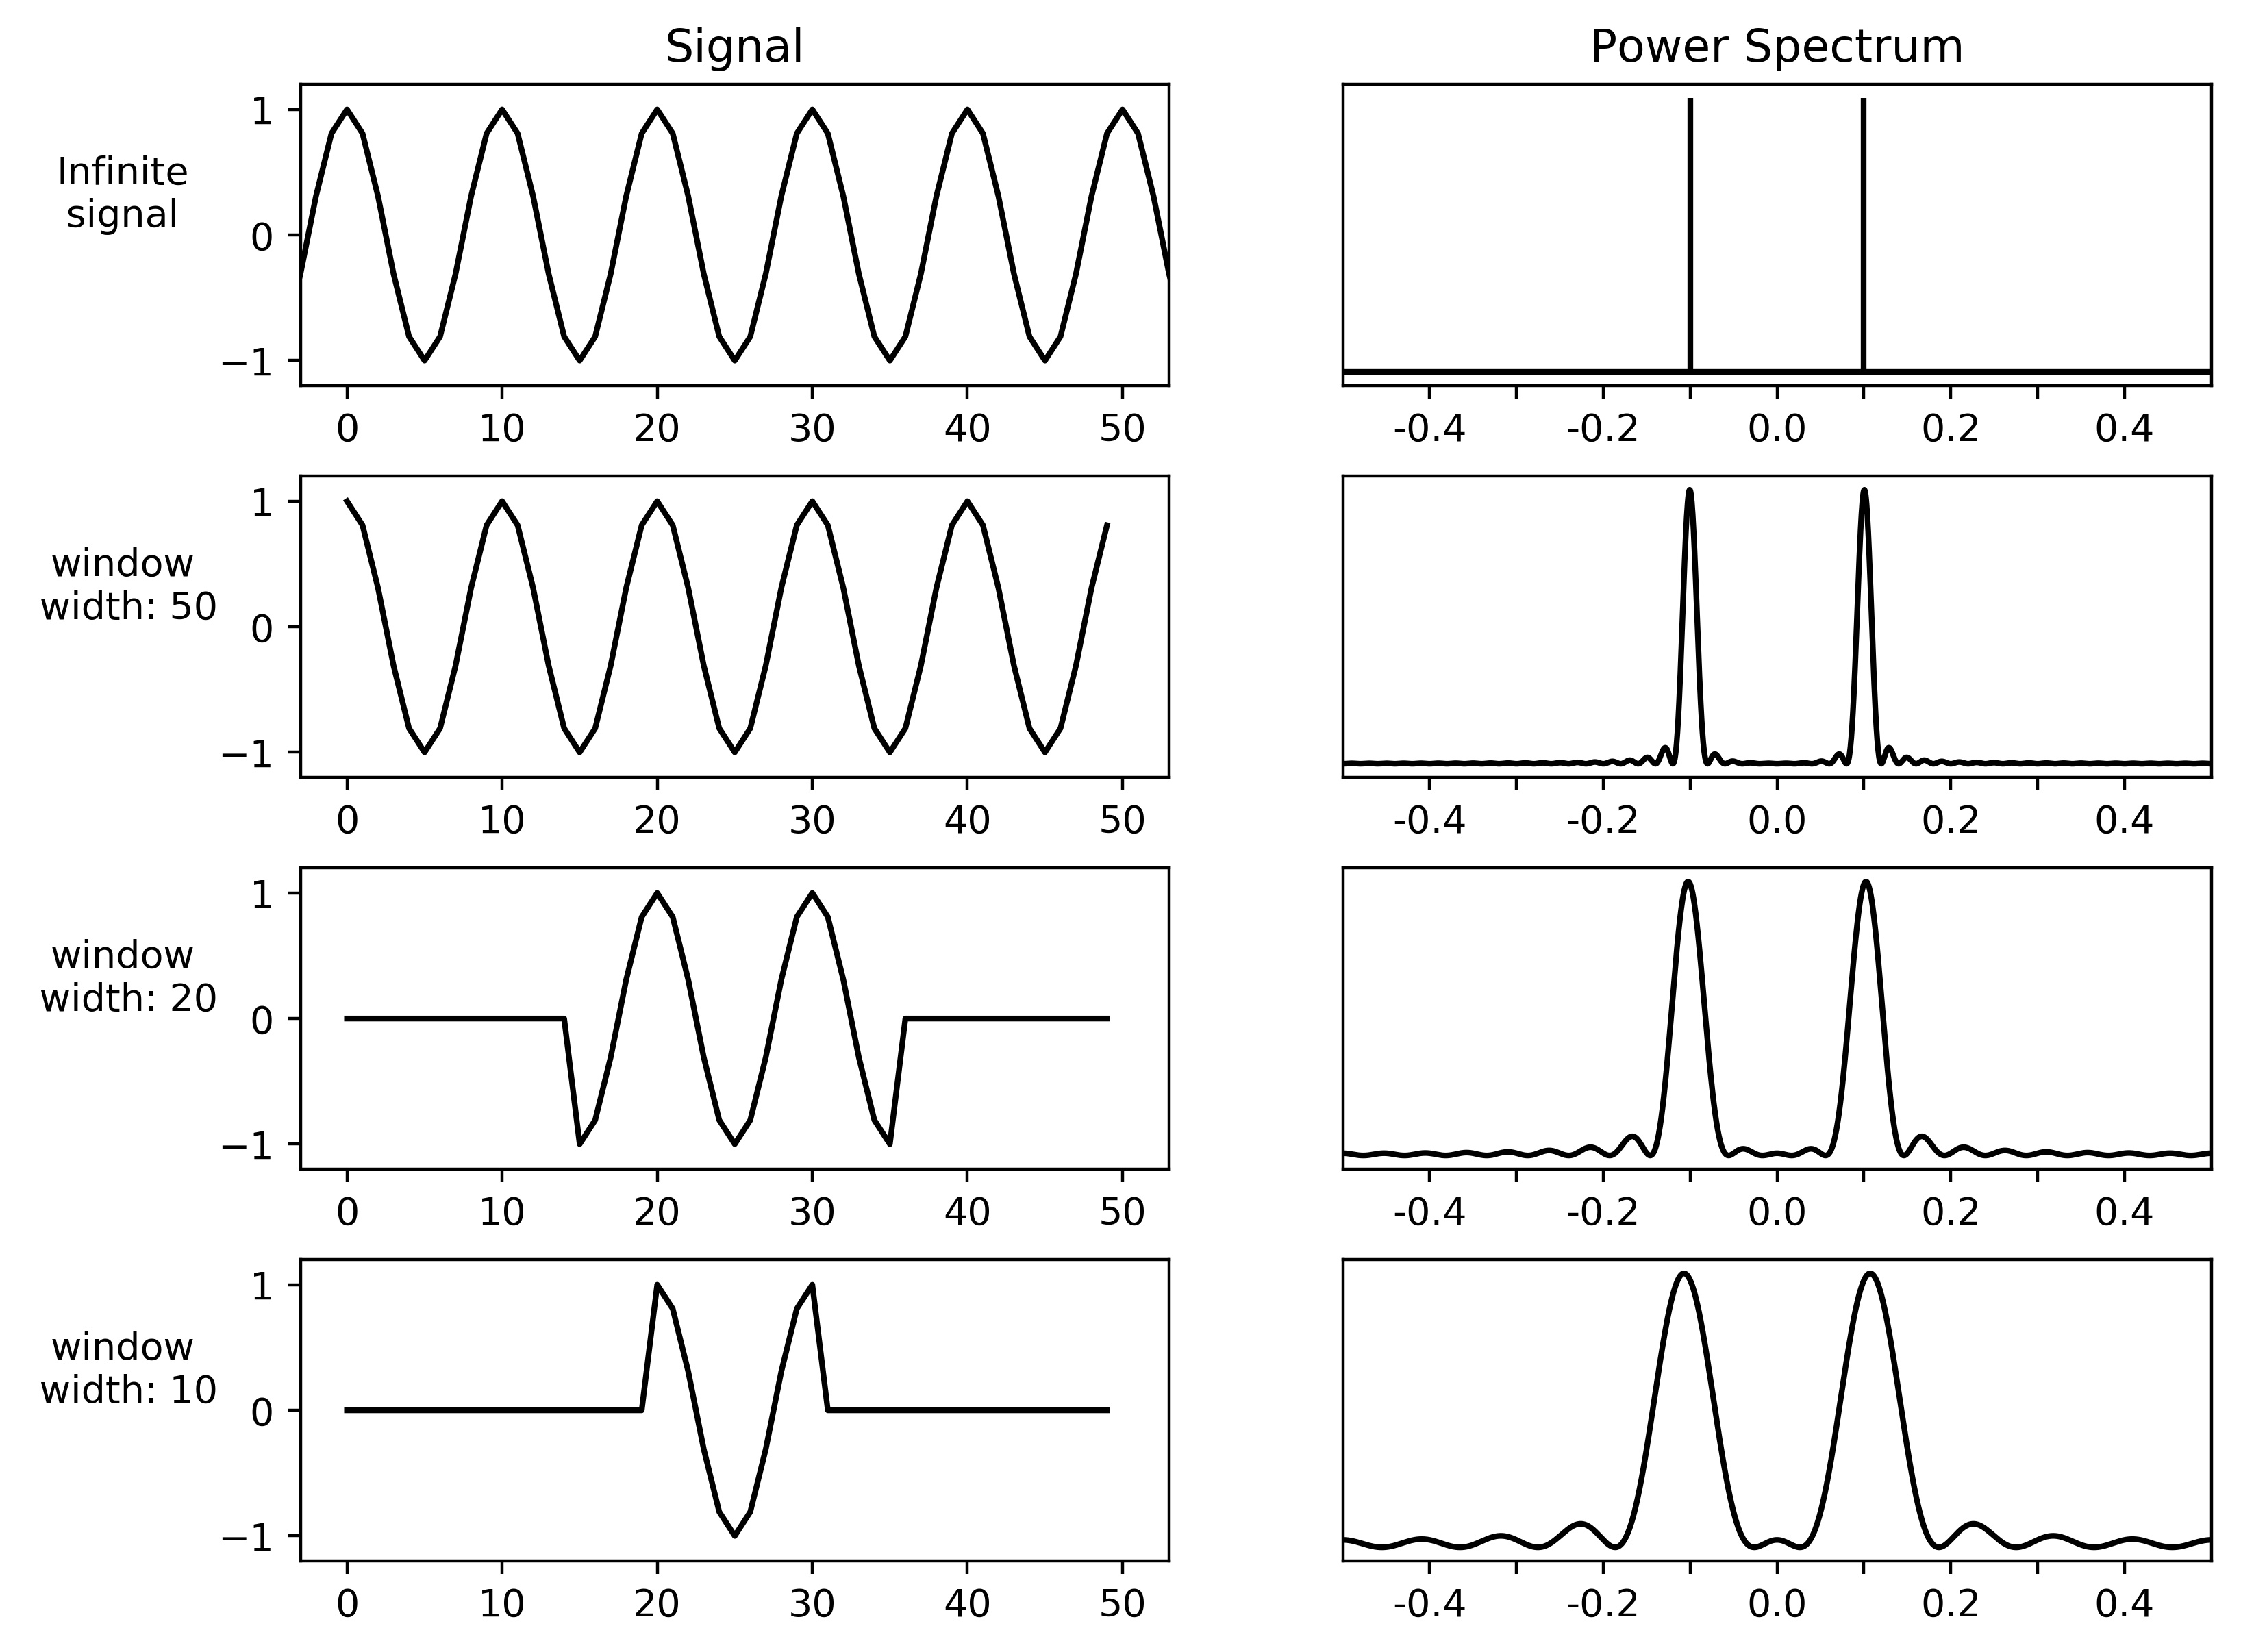
\includegraphics[scale=0.55]{Figuras/fig1.jpg}
\end{center}
\end{frame}

%%%%%%%%%%%%%%%%%%%%%%%%  FRAME  %%%%%%%%%%%%%%%%%%%%%%%%
\begin{frame}
\frametitle{Effects of sampling rate - aliasing (a kind of leakage)}
\begin{center}
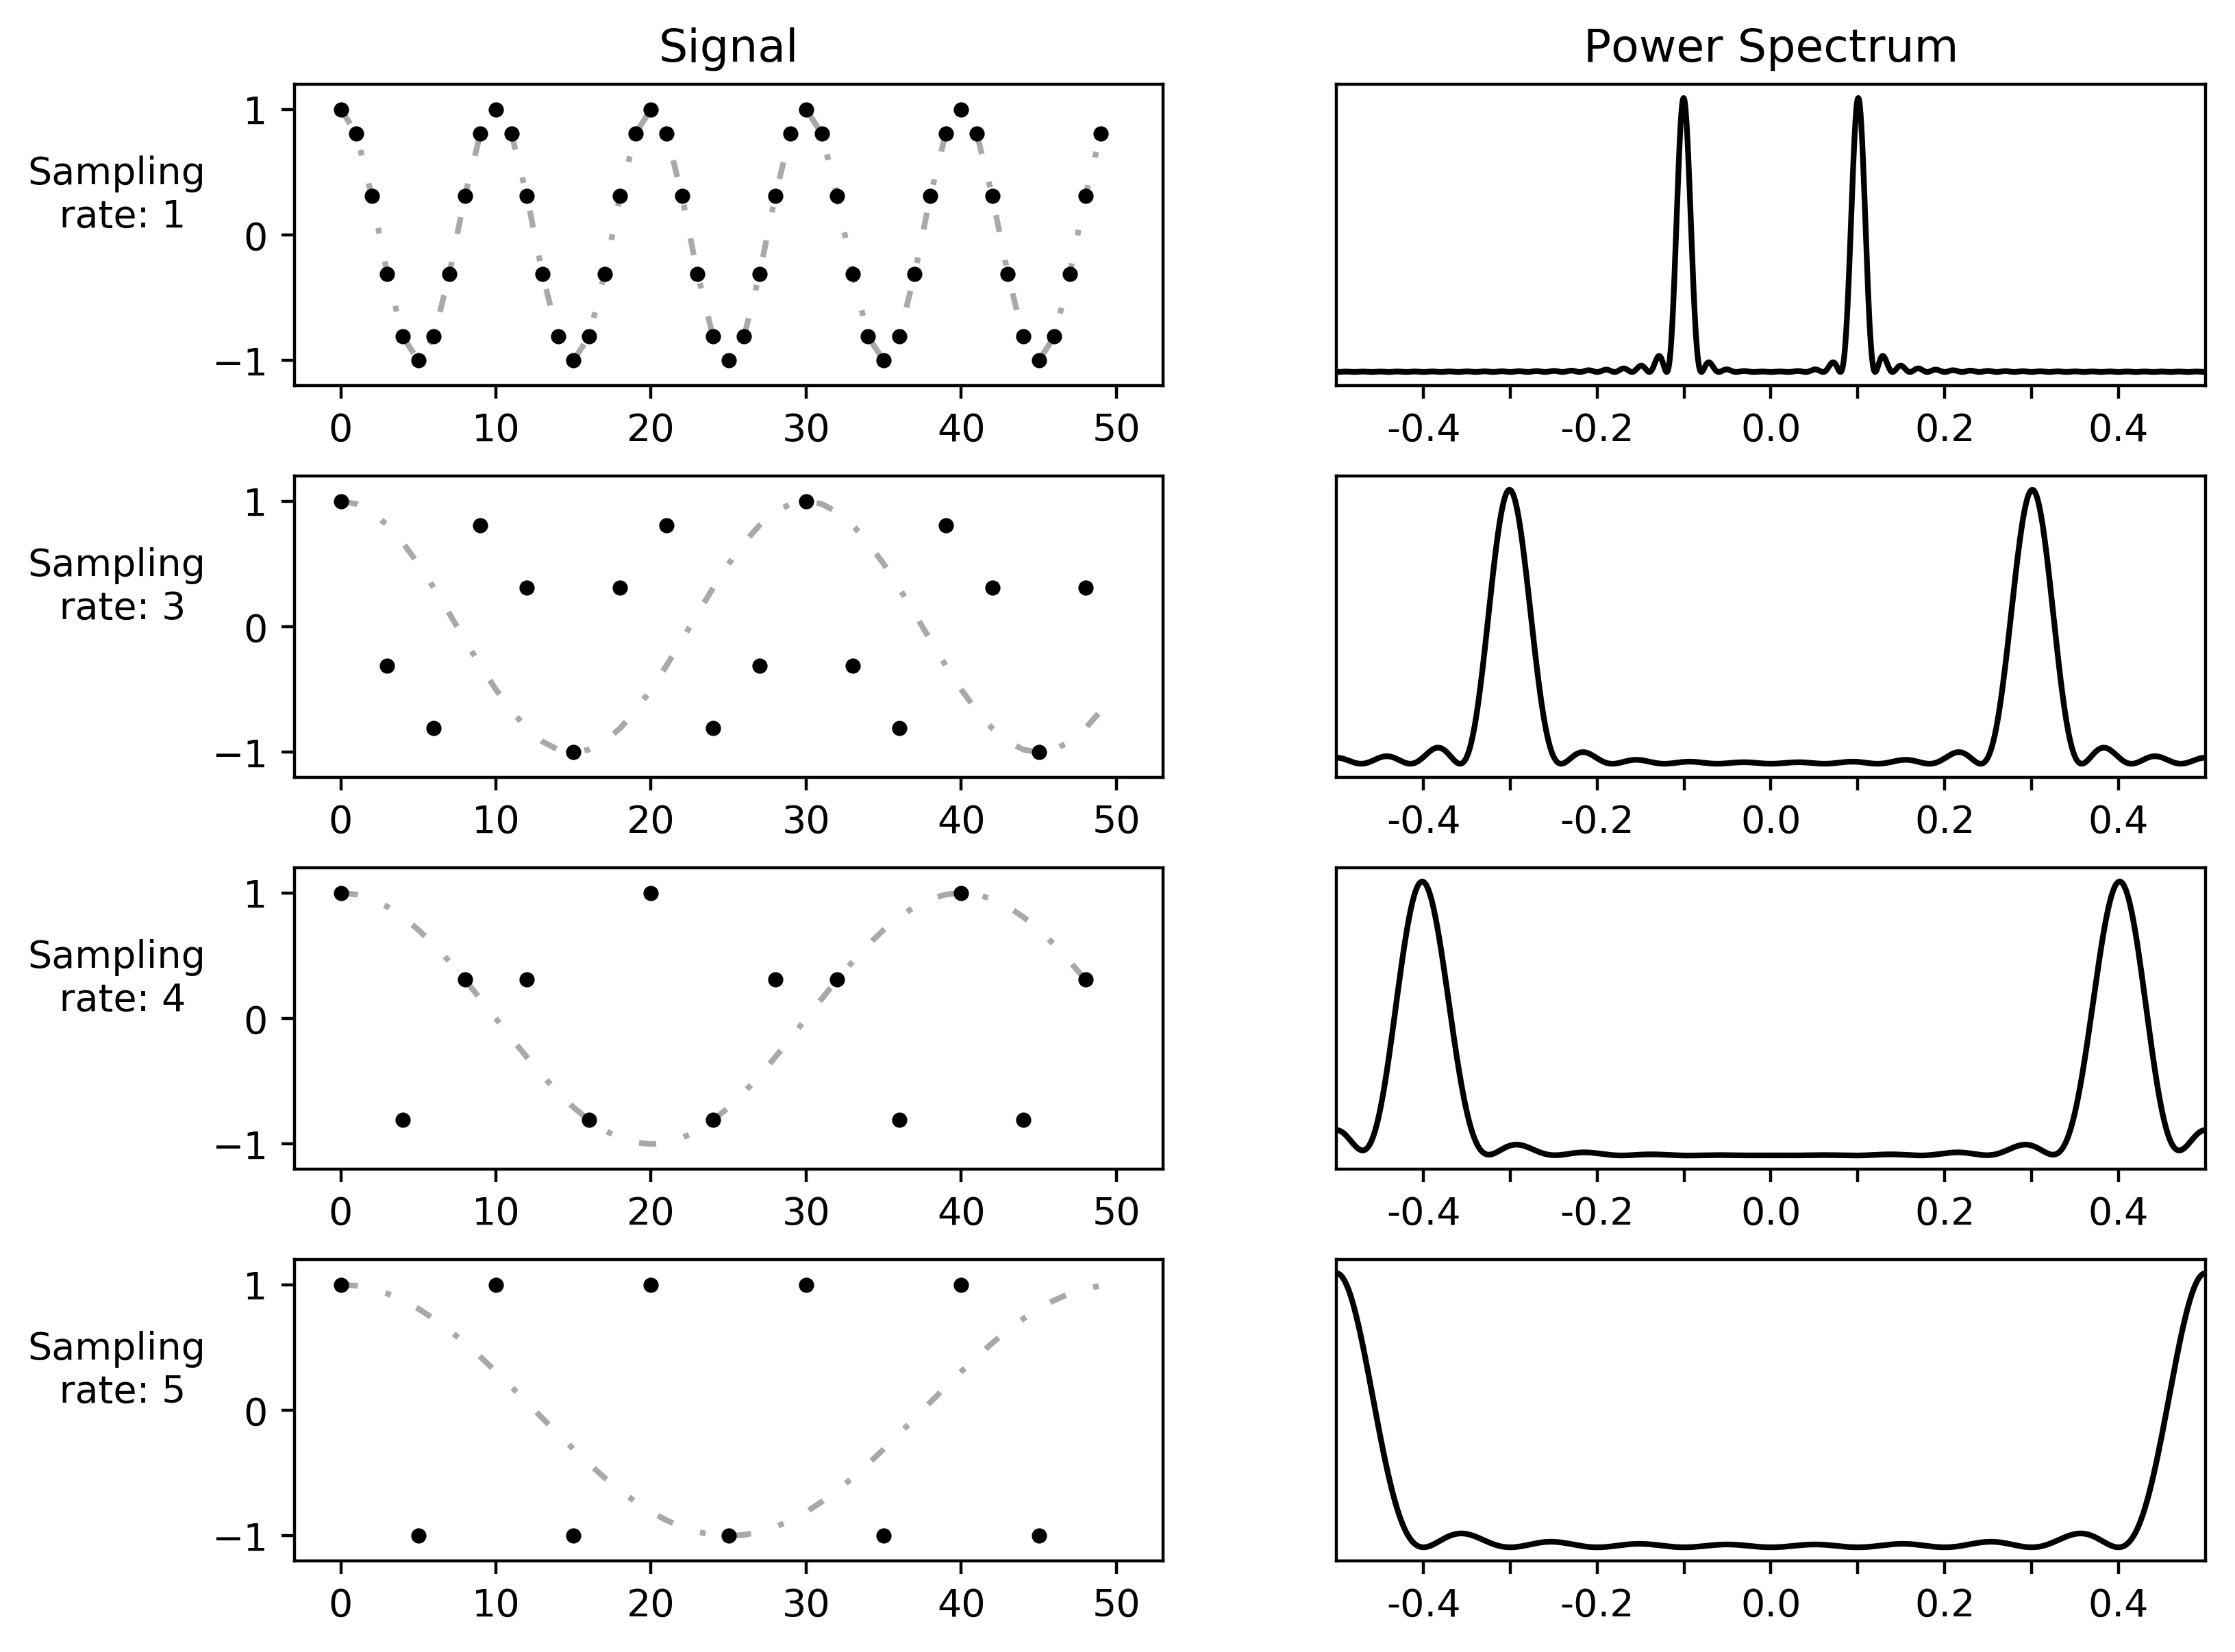
\includegraphics[scale=0.55]{Figuras/fig2.jpg}
\end{center}
\end{frame}

%%%%%%%%%%%%%%%%%%%%%%%%  FRAME  %%%%%%%%%%%%%%%%%%%%%%%%
\begin{frame}
\frametitle{Effects of non-uniform sampling}
\begin{center}
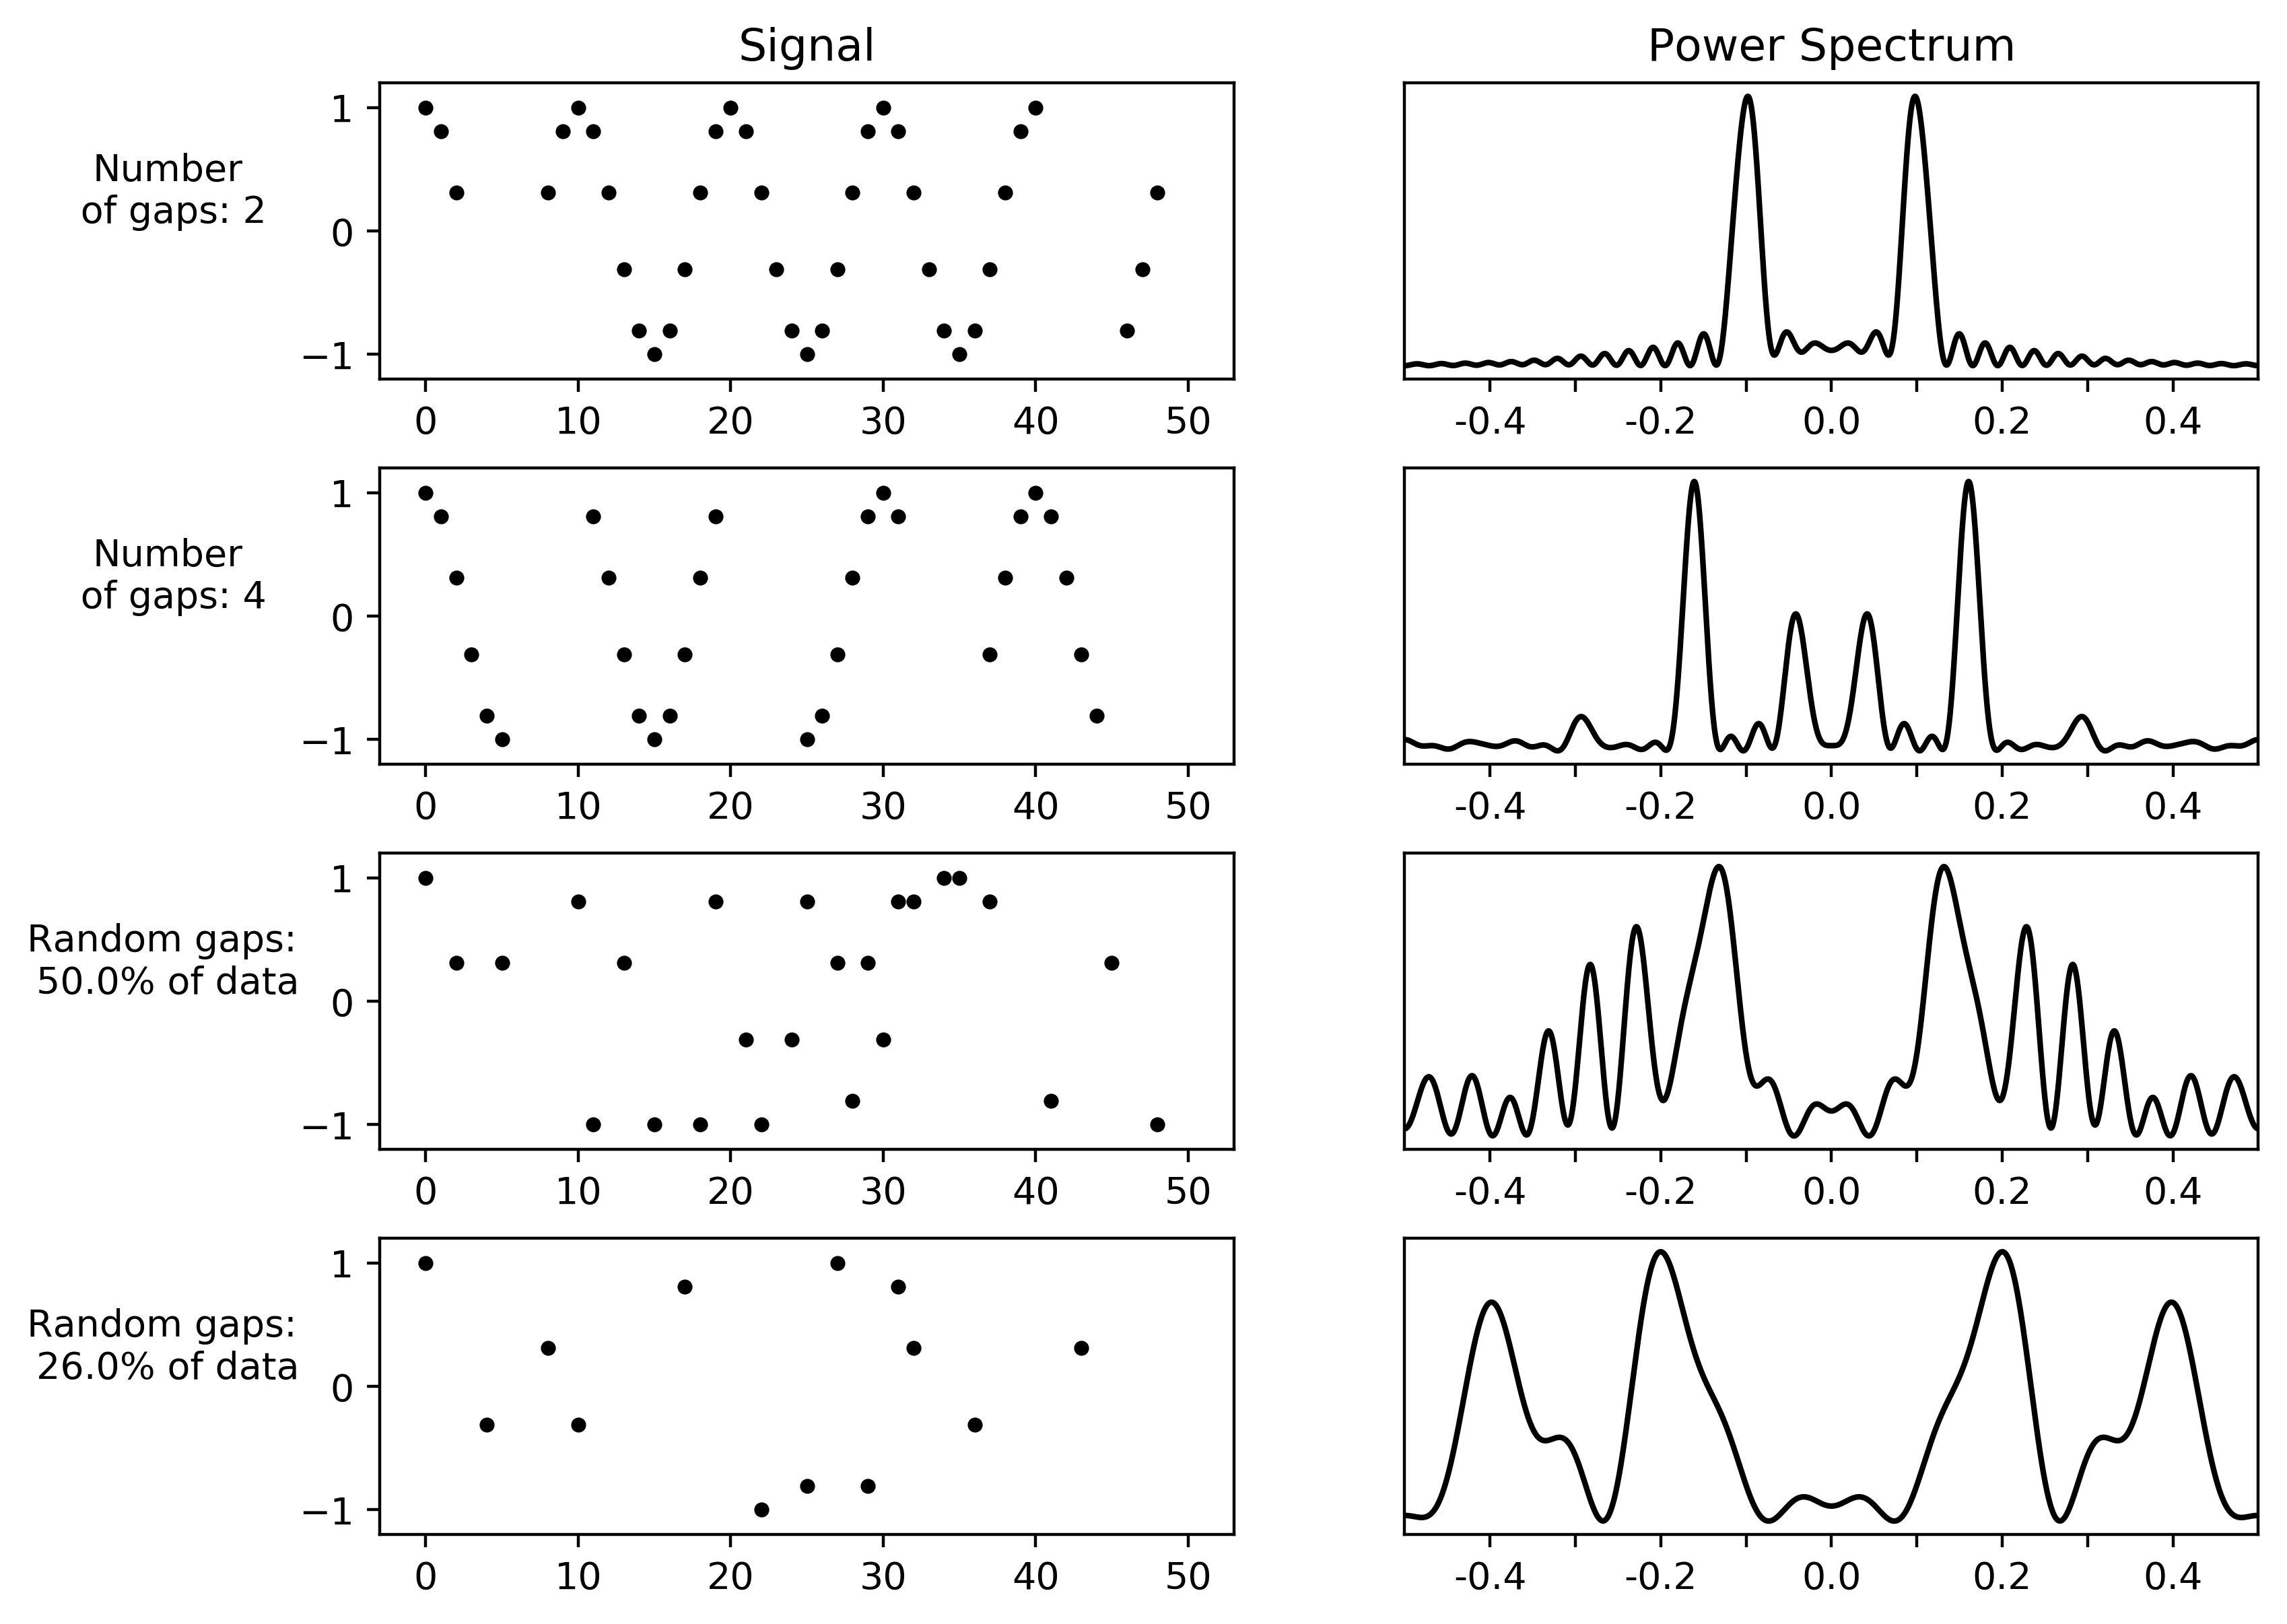
\includegraphics[scale=0.55]{Figuras/fig3.jpg}
\end{center}
\end{frame}

\section{The Lomb-Scargle tool}

%%%%%%%%%%%%%%%%%%%%%%%%  FRAME  %%%%%%%%%%%%%%%%%%%%%%%%
\begin{frame}[fragile]
\frametitle{Lomb-Scargle periodogram}
\begin{itemize}
\item Main tool for analysis of unevenly sampled temporal series 
\item Belongs to a set of tools of spectral analysis that explores the least squares method
\item Estimates frequencies by fitting sinusoidal functions to the data
\item Available via the library \texttt{astropy} (with $O[NlogN]$ complexity) via the class \texttt{LombScargle}:
\begin{lstlisting}[language=python,style=mystyle2]
from astropy.timeseries import LombScargle
frequency, power = LombScargle(t, f).autopower()
\end{lstlisting}
\end{itemize}
\end{frame}

\section{Results}

%%%%%%%%%%%%%%%%%%%%%%%%  FRAME  %%%%%%%%%%%%%%%%%%%%%%%%
\begin{frame}
\frametitle{The analysis}
\begin{itemize}
\item Scenario 1
\begin{itemize}
\item Gaps (of data) randomly placed in the original series
\item Size of gaps equal to 10\% of data
\item Five number of gaps tested
\end{itemize}
\item Scenario 2
\begin{itemize}
\item Data randomly deleted from the original series
\item Deletion of a particular percentage 
\item Five percentages are tested
\end{itemize}
\end{itemize}
\end{frame}

%%%%%%%%%%%%%%%%%%%%%%%%  FRAME  %%%%%%%%%%%%%%%%%%%%%%%%
\begin{frame}
\frametitle{Power spectrum via FFT - the usual analysis}
\begin{center}
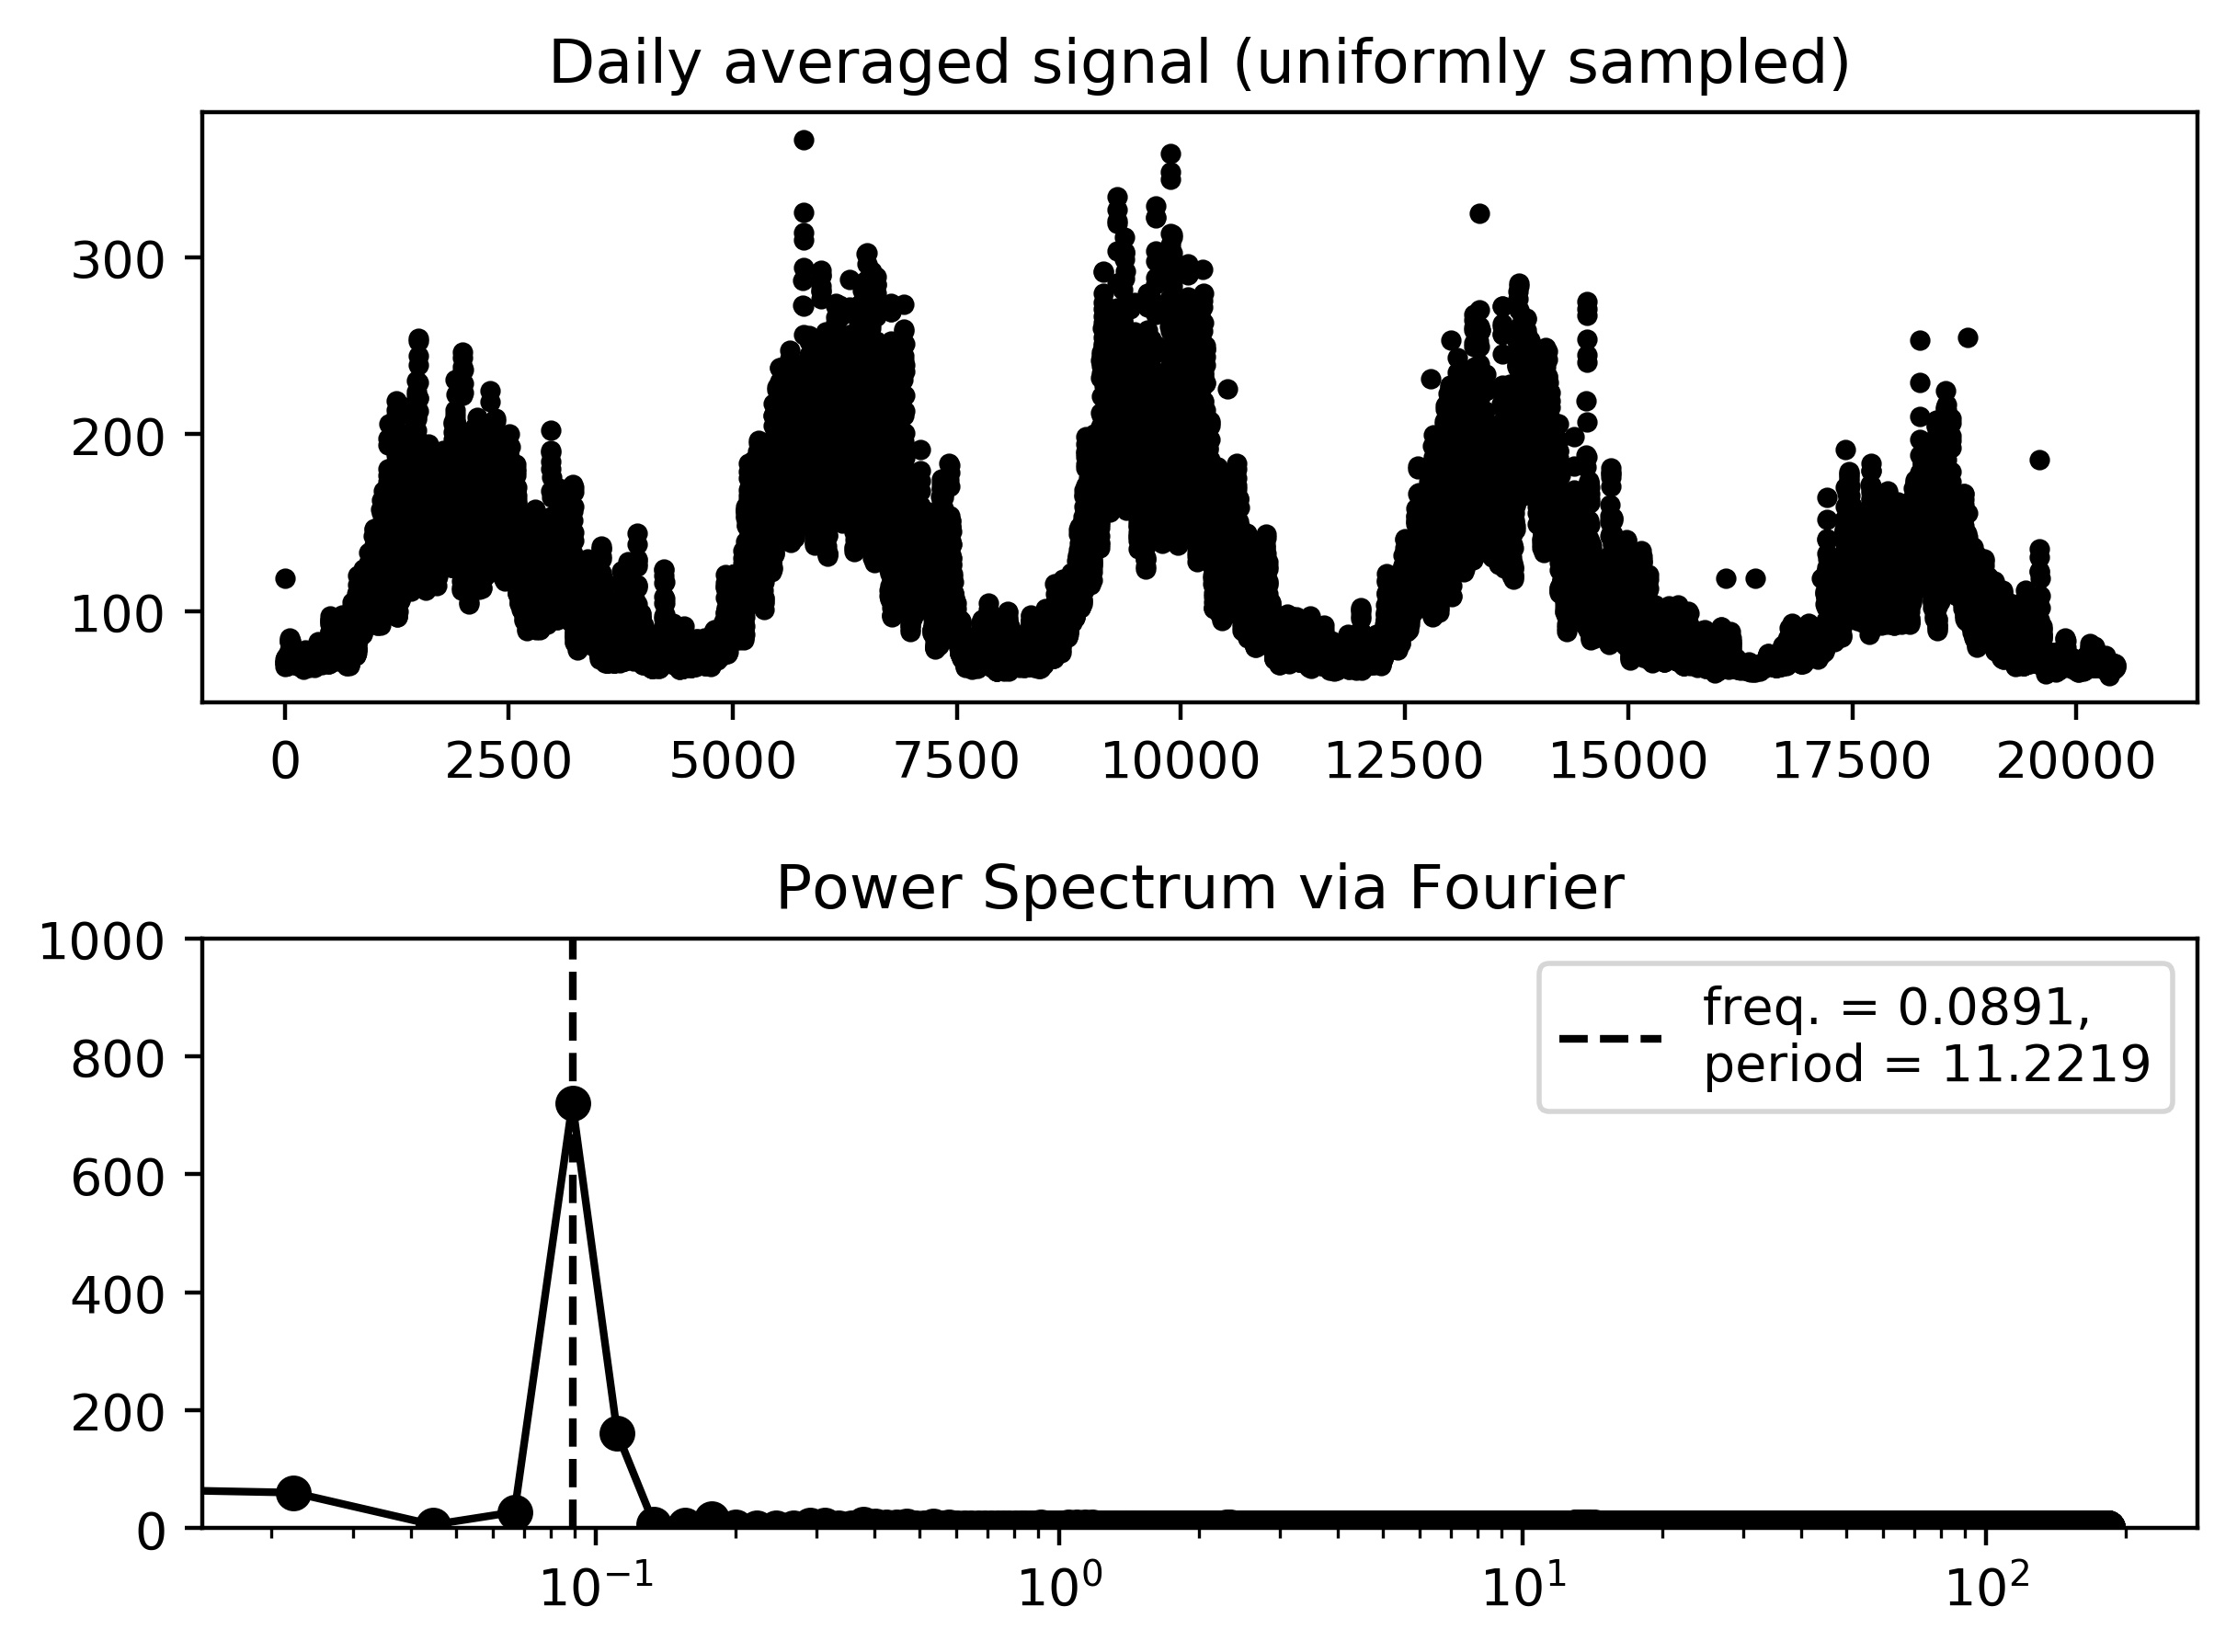
\includegraphics[scale=0.55]{Figuras/original_365.jpg}
\end{center}
\end{frame}

%%%%%%%%%%%%%%%%%%%%%%%%  FRAME  %%%%%%%%%%%%%%%%%%%%%%%%
\begin{frame}
\frametitle{Scenario 1 - daily averages}
\begin{center}
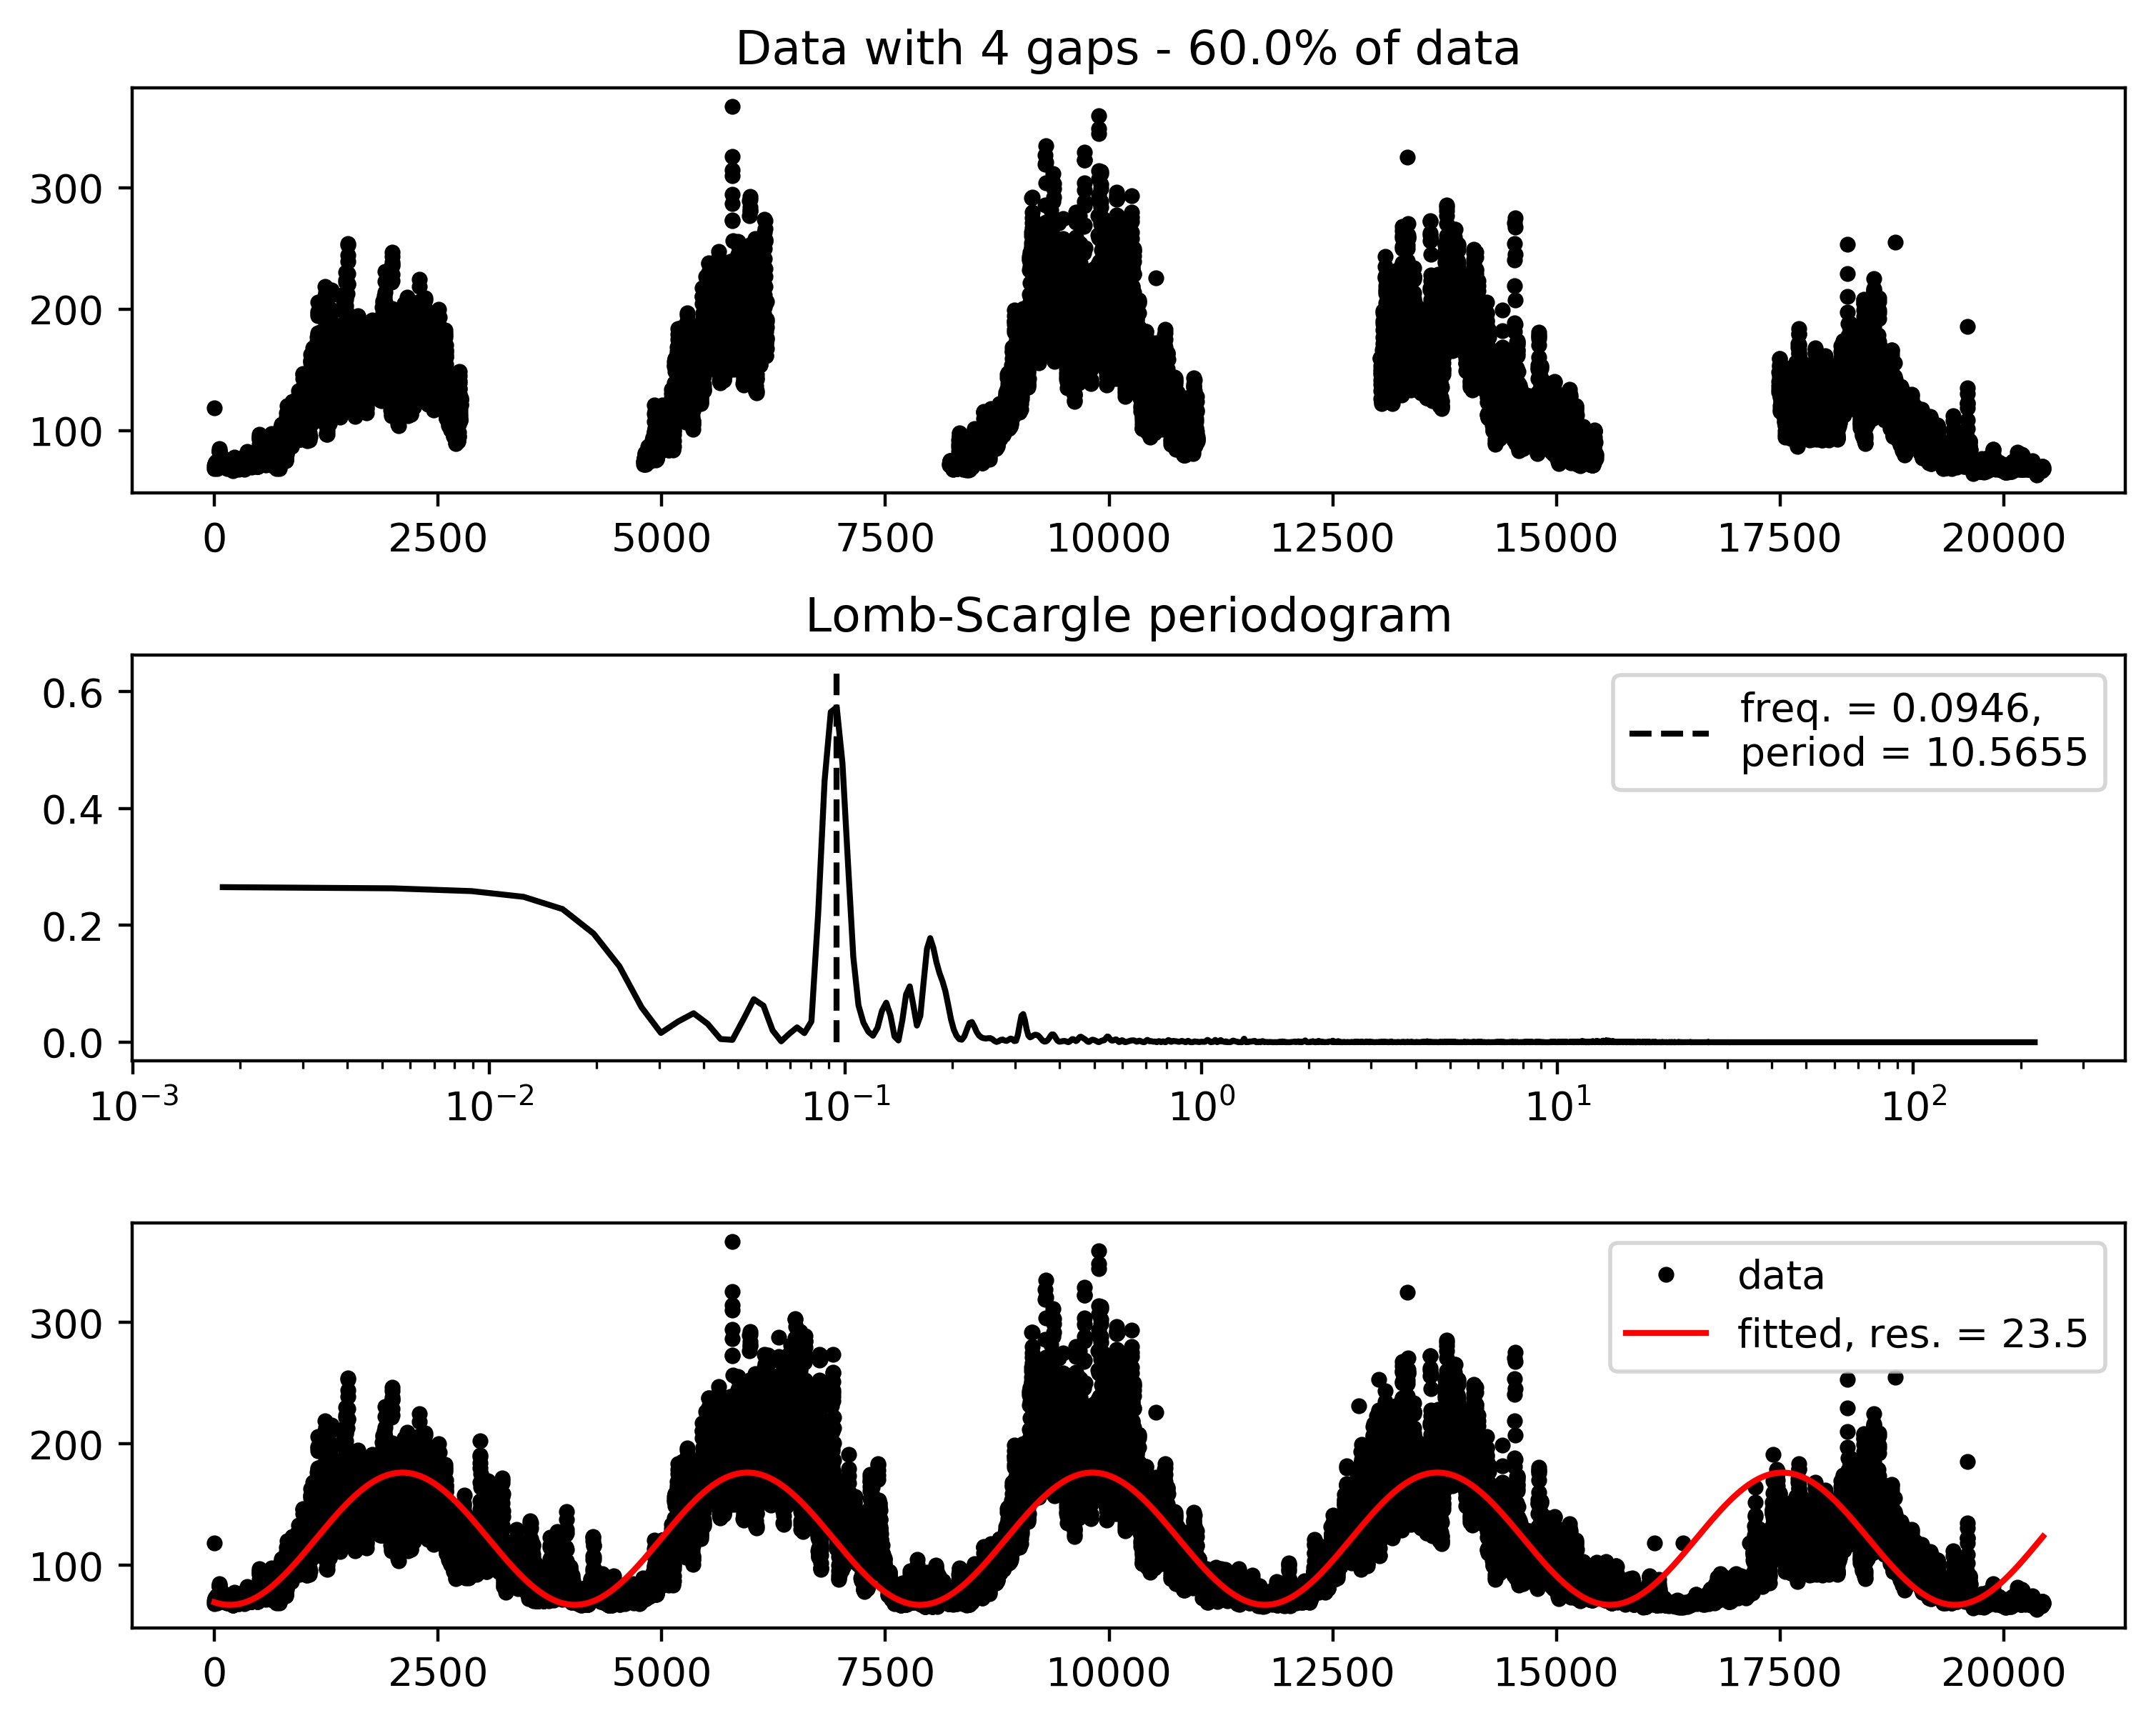
\includegraphics[scale=0.55]{../scripts/dataset1/periodograms_ny2.0_model2_Ng4.jpg}
\end{center}
\end{frame}
\begin{frame}
\frametitle{Scenario 1 - daily averages}
\begin{center}
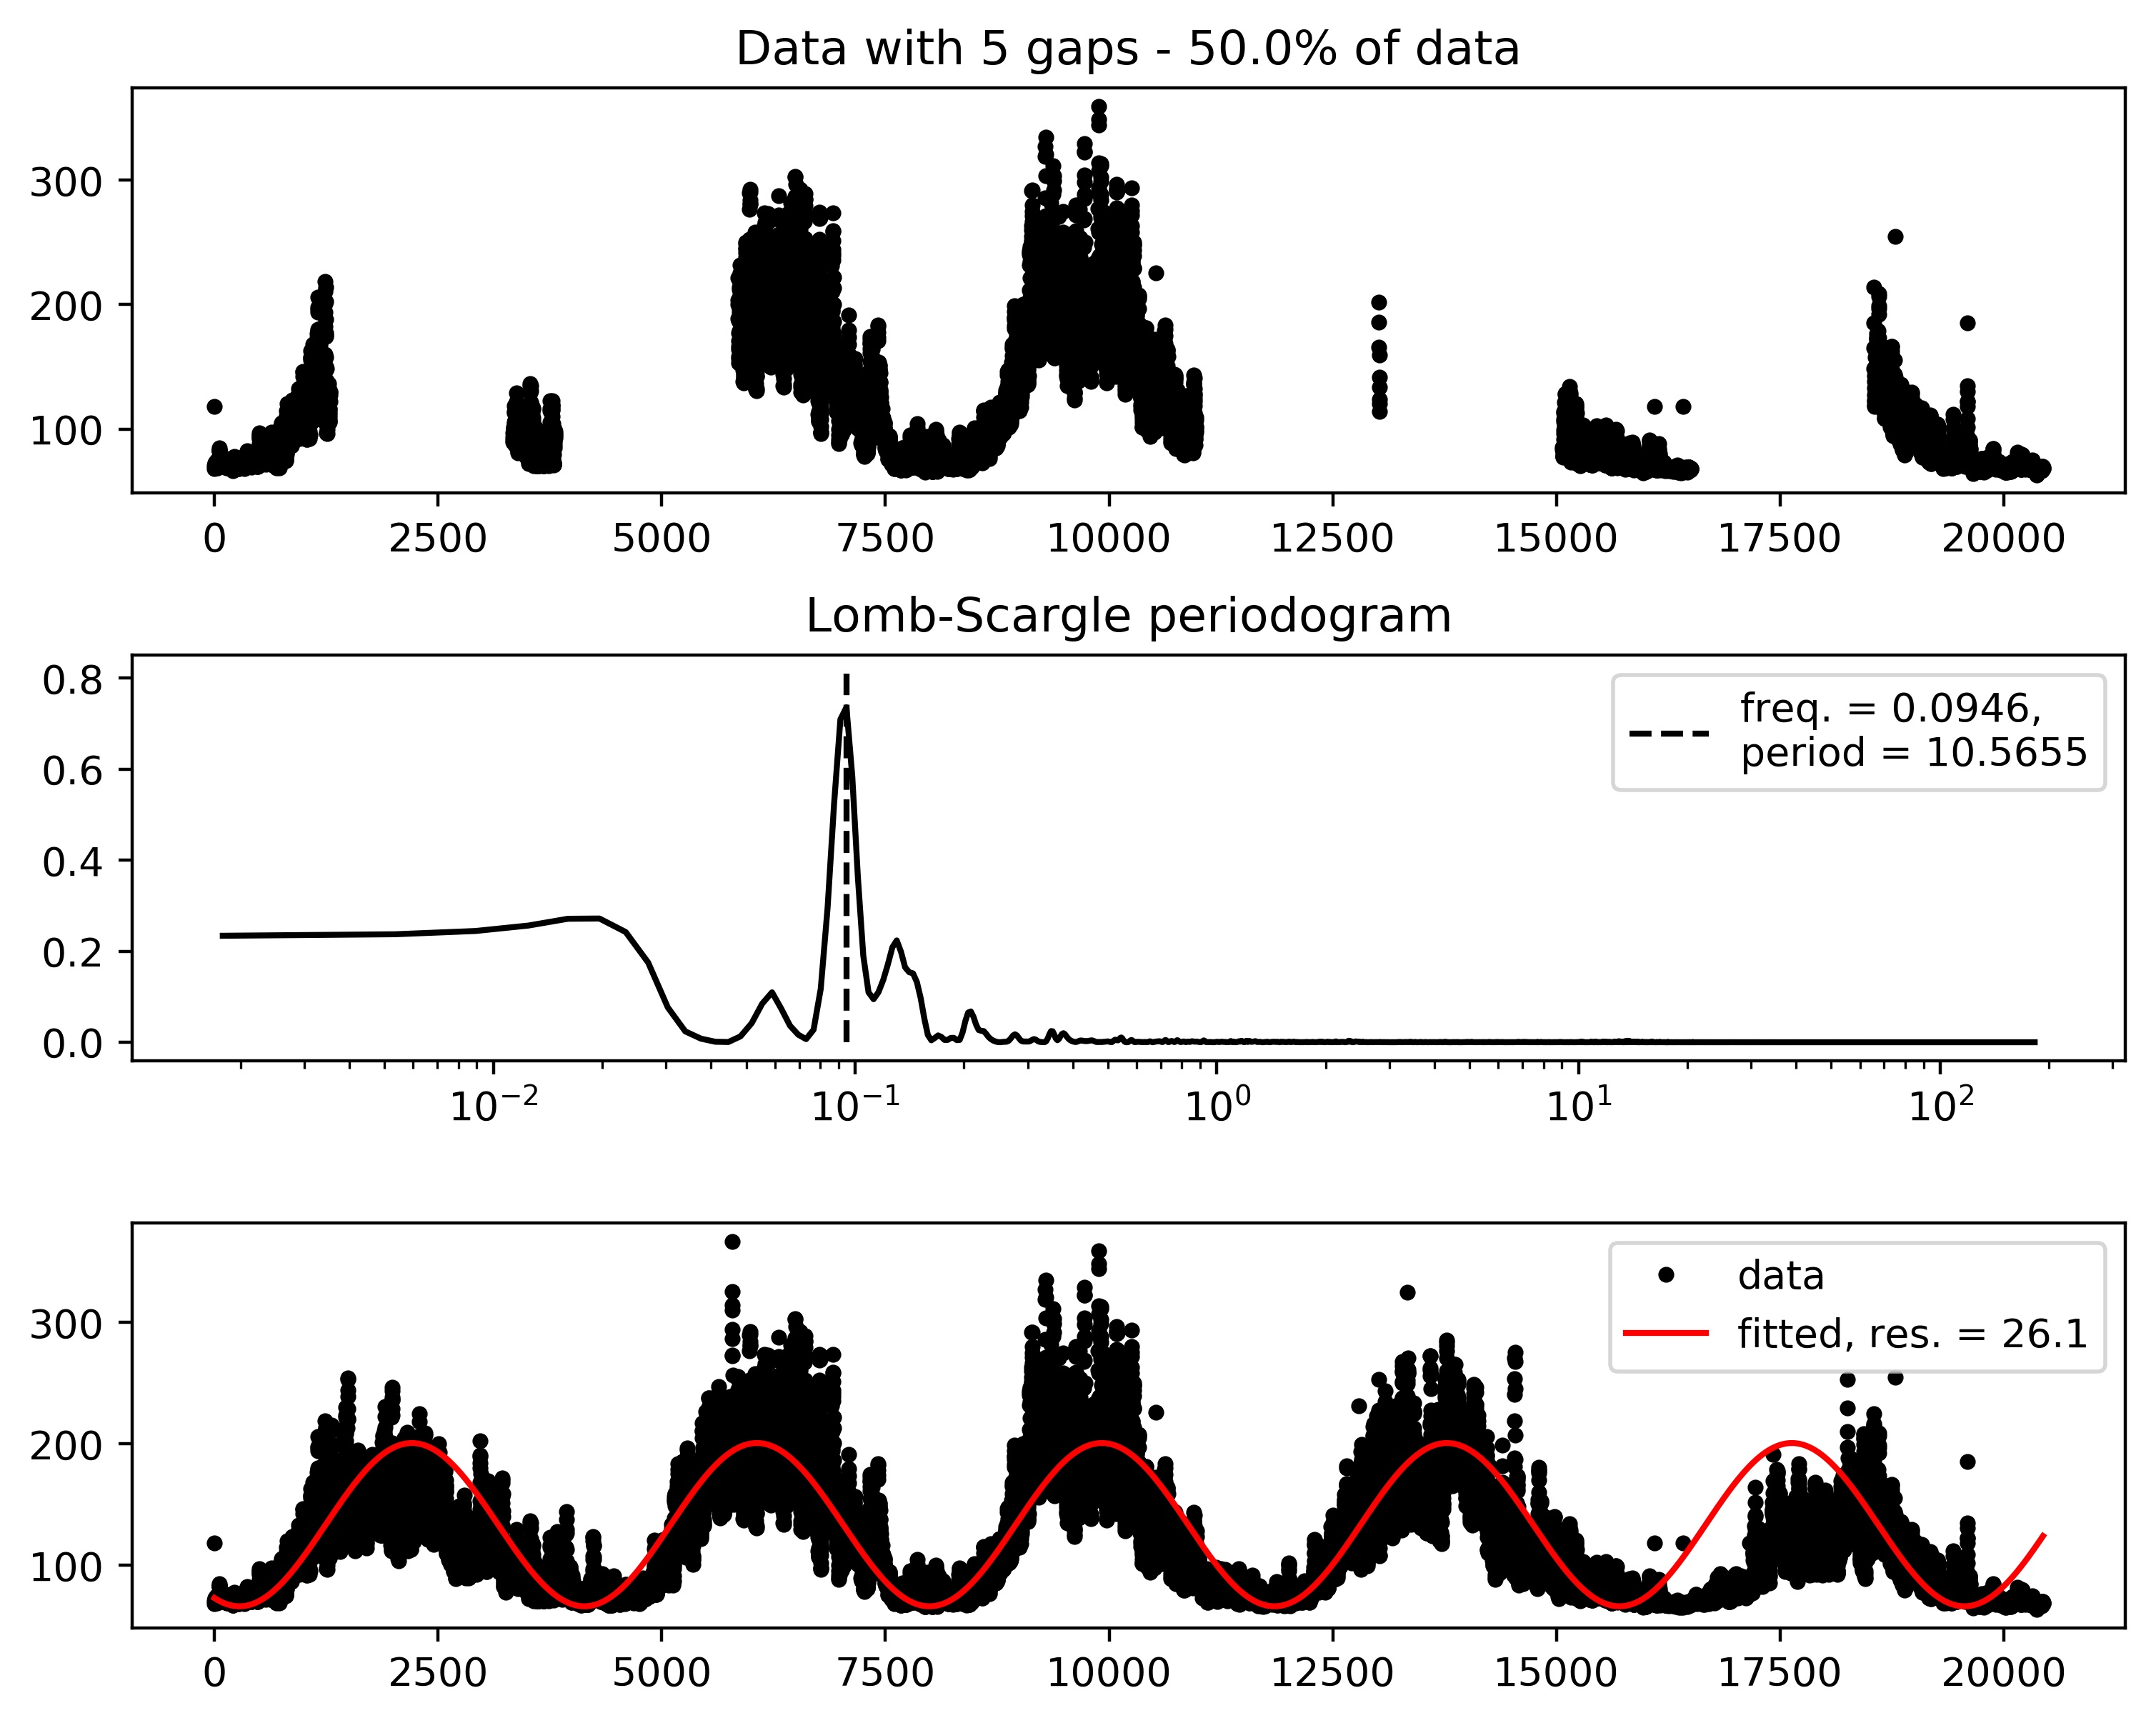
\includegraphics[scale=0.55]{../scripts/dataset1/periodograms_ny2.0_model2_Ng5.jpg}
\end{center}
\end{frame}
\begin{frame}
\frametitle{Scenario 1 - daily averages}
\begin{center}
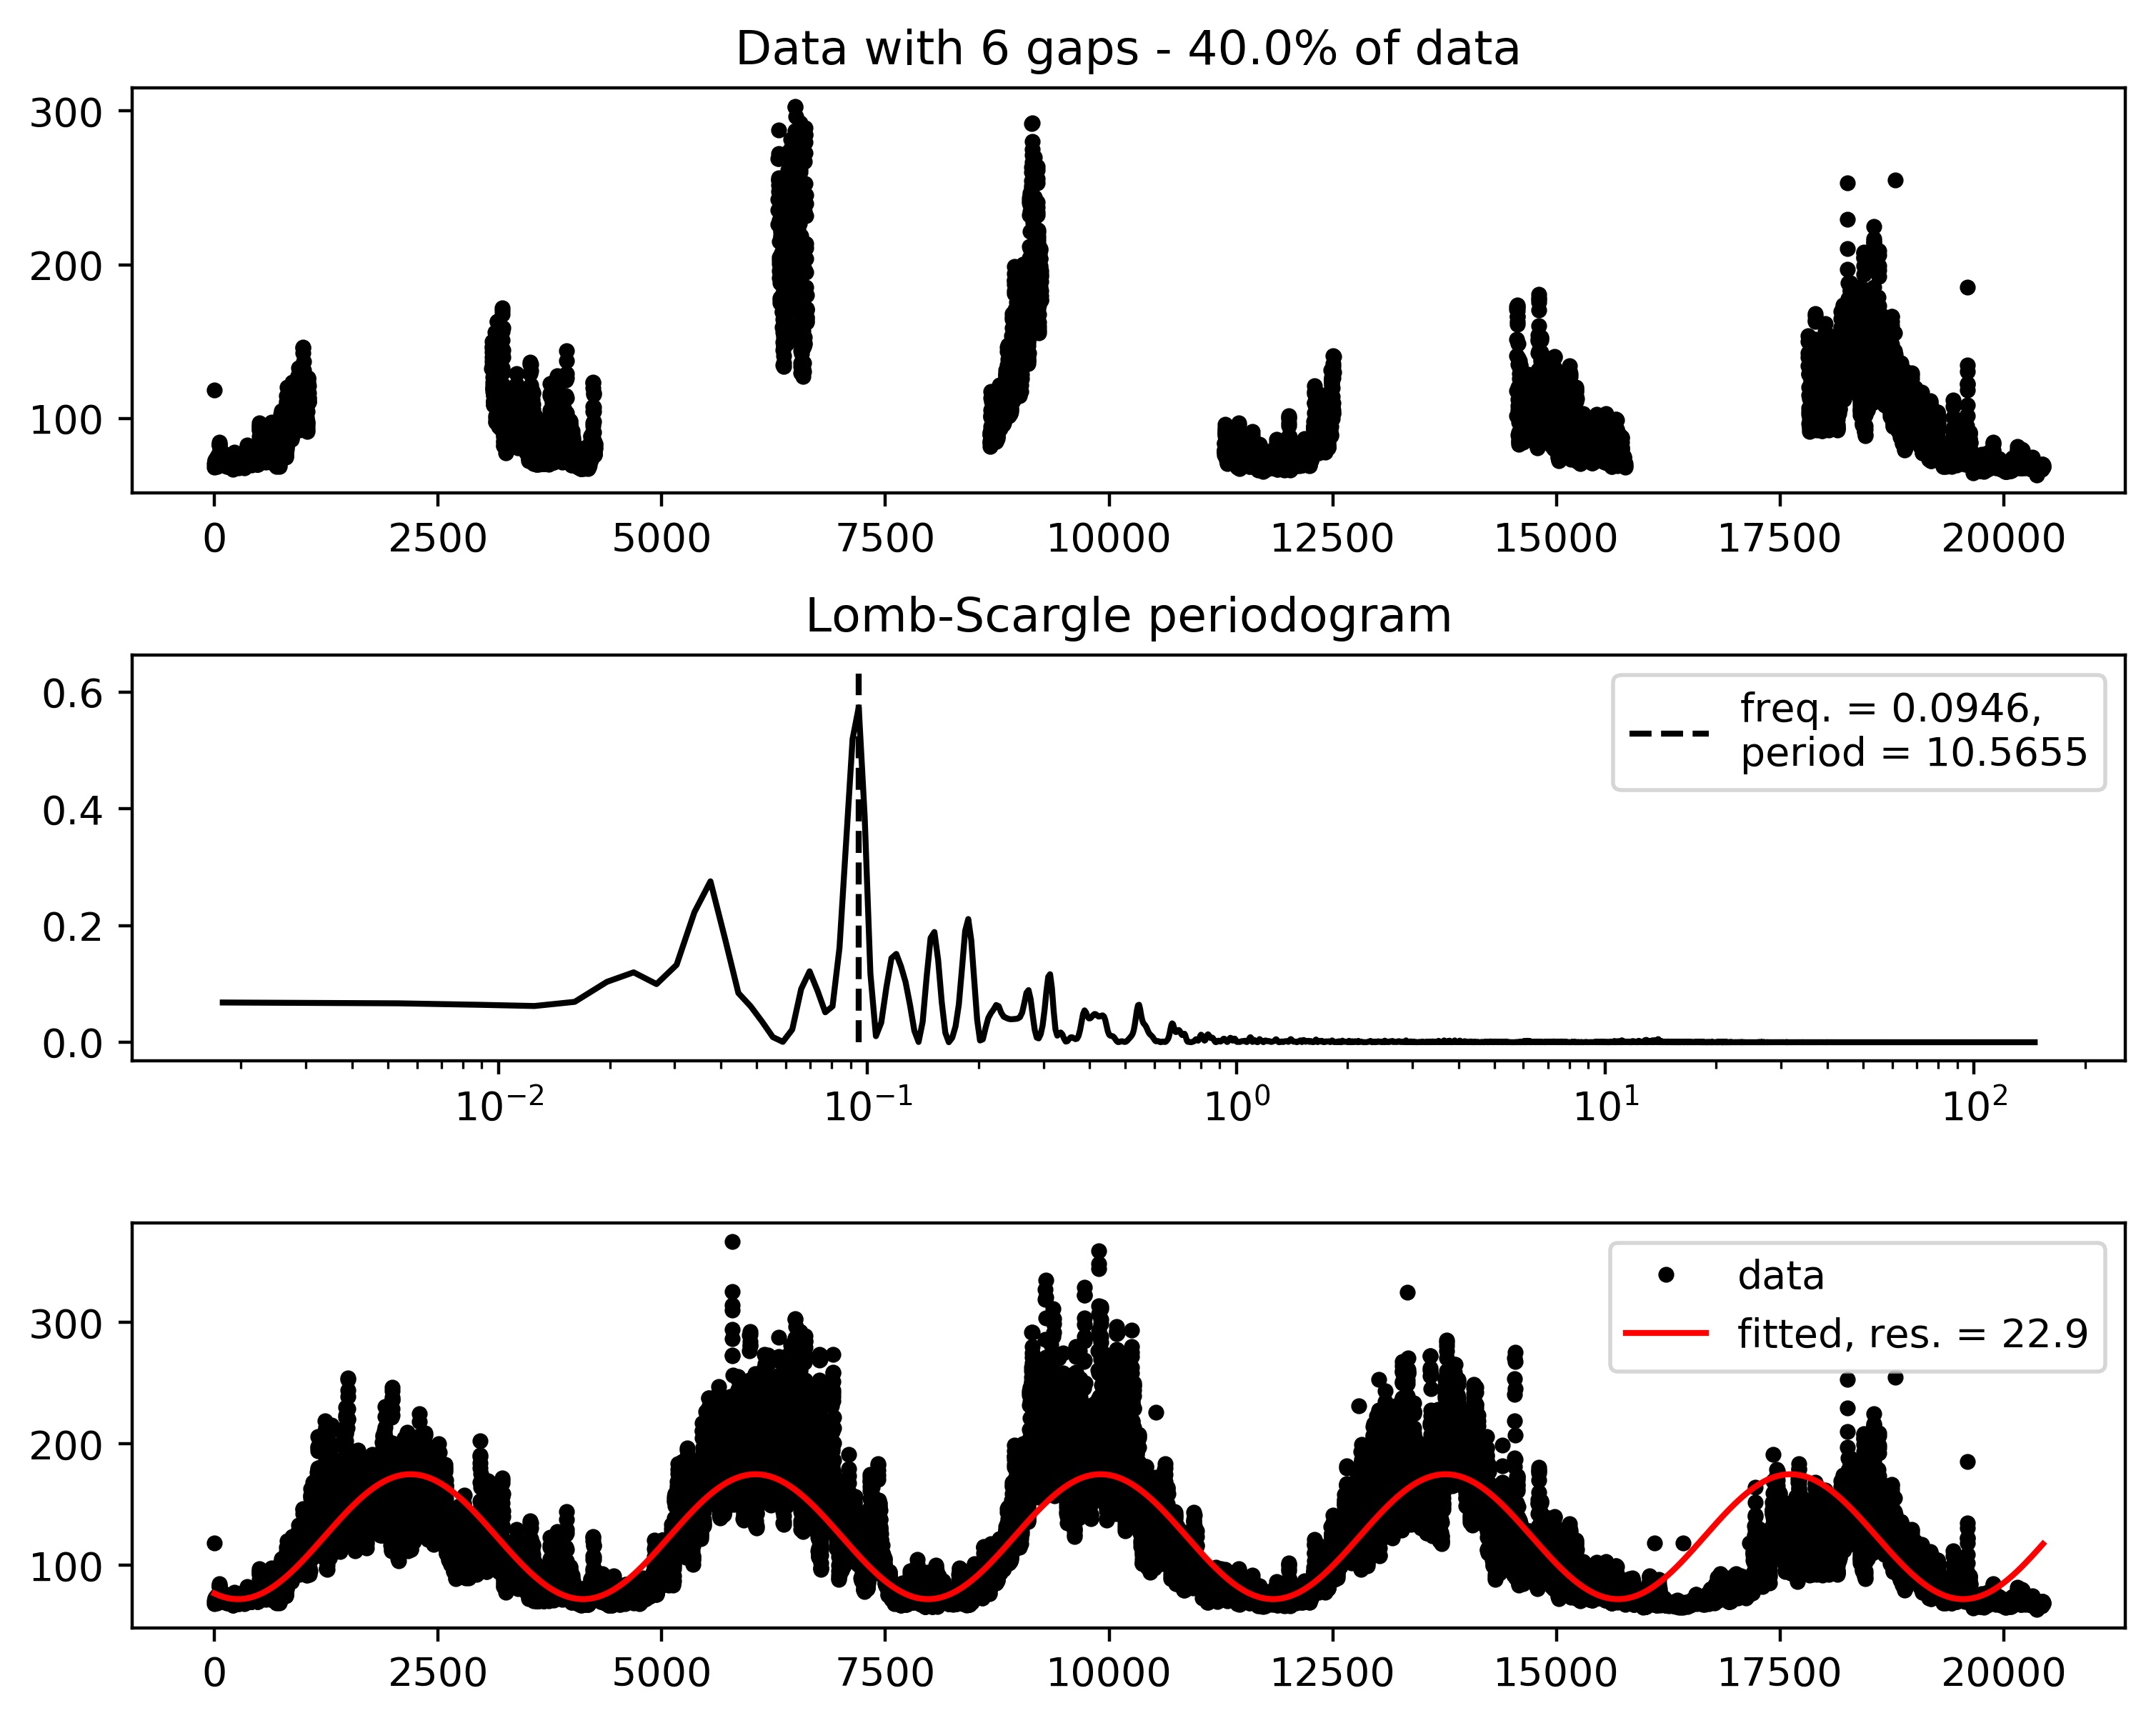
\includegraphics[scale=0.55]{../scripts/dataset1/periodograms_ny2.0_model2_Ng6.jpg}
\end{center}
\end{frame}
\begin{frame}
\frametitle{Scenario 1 - daily averages}
\begin{center}
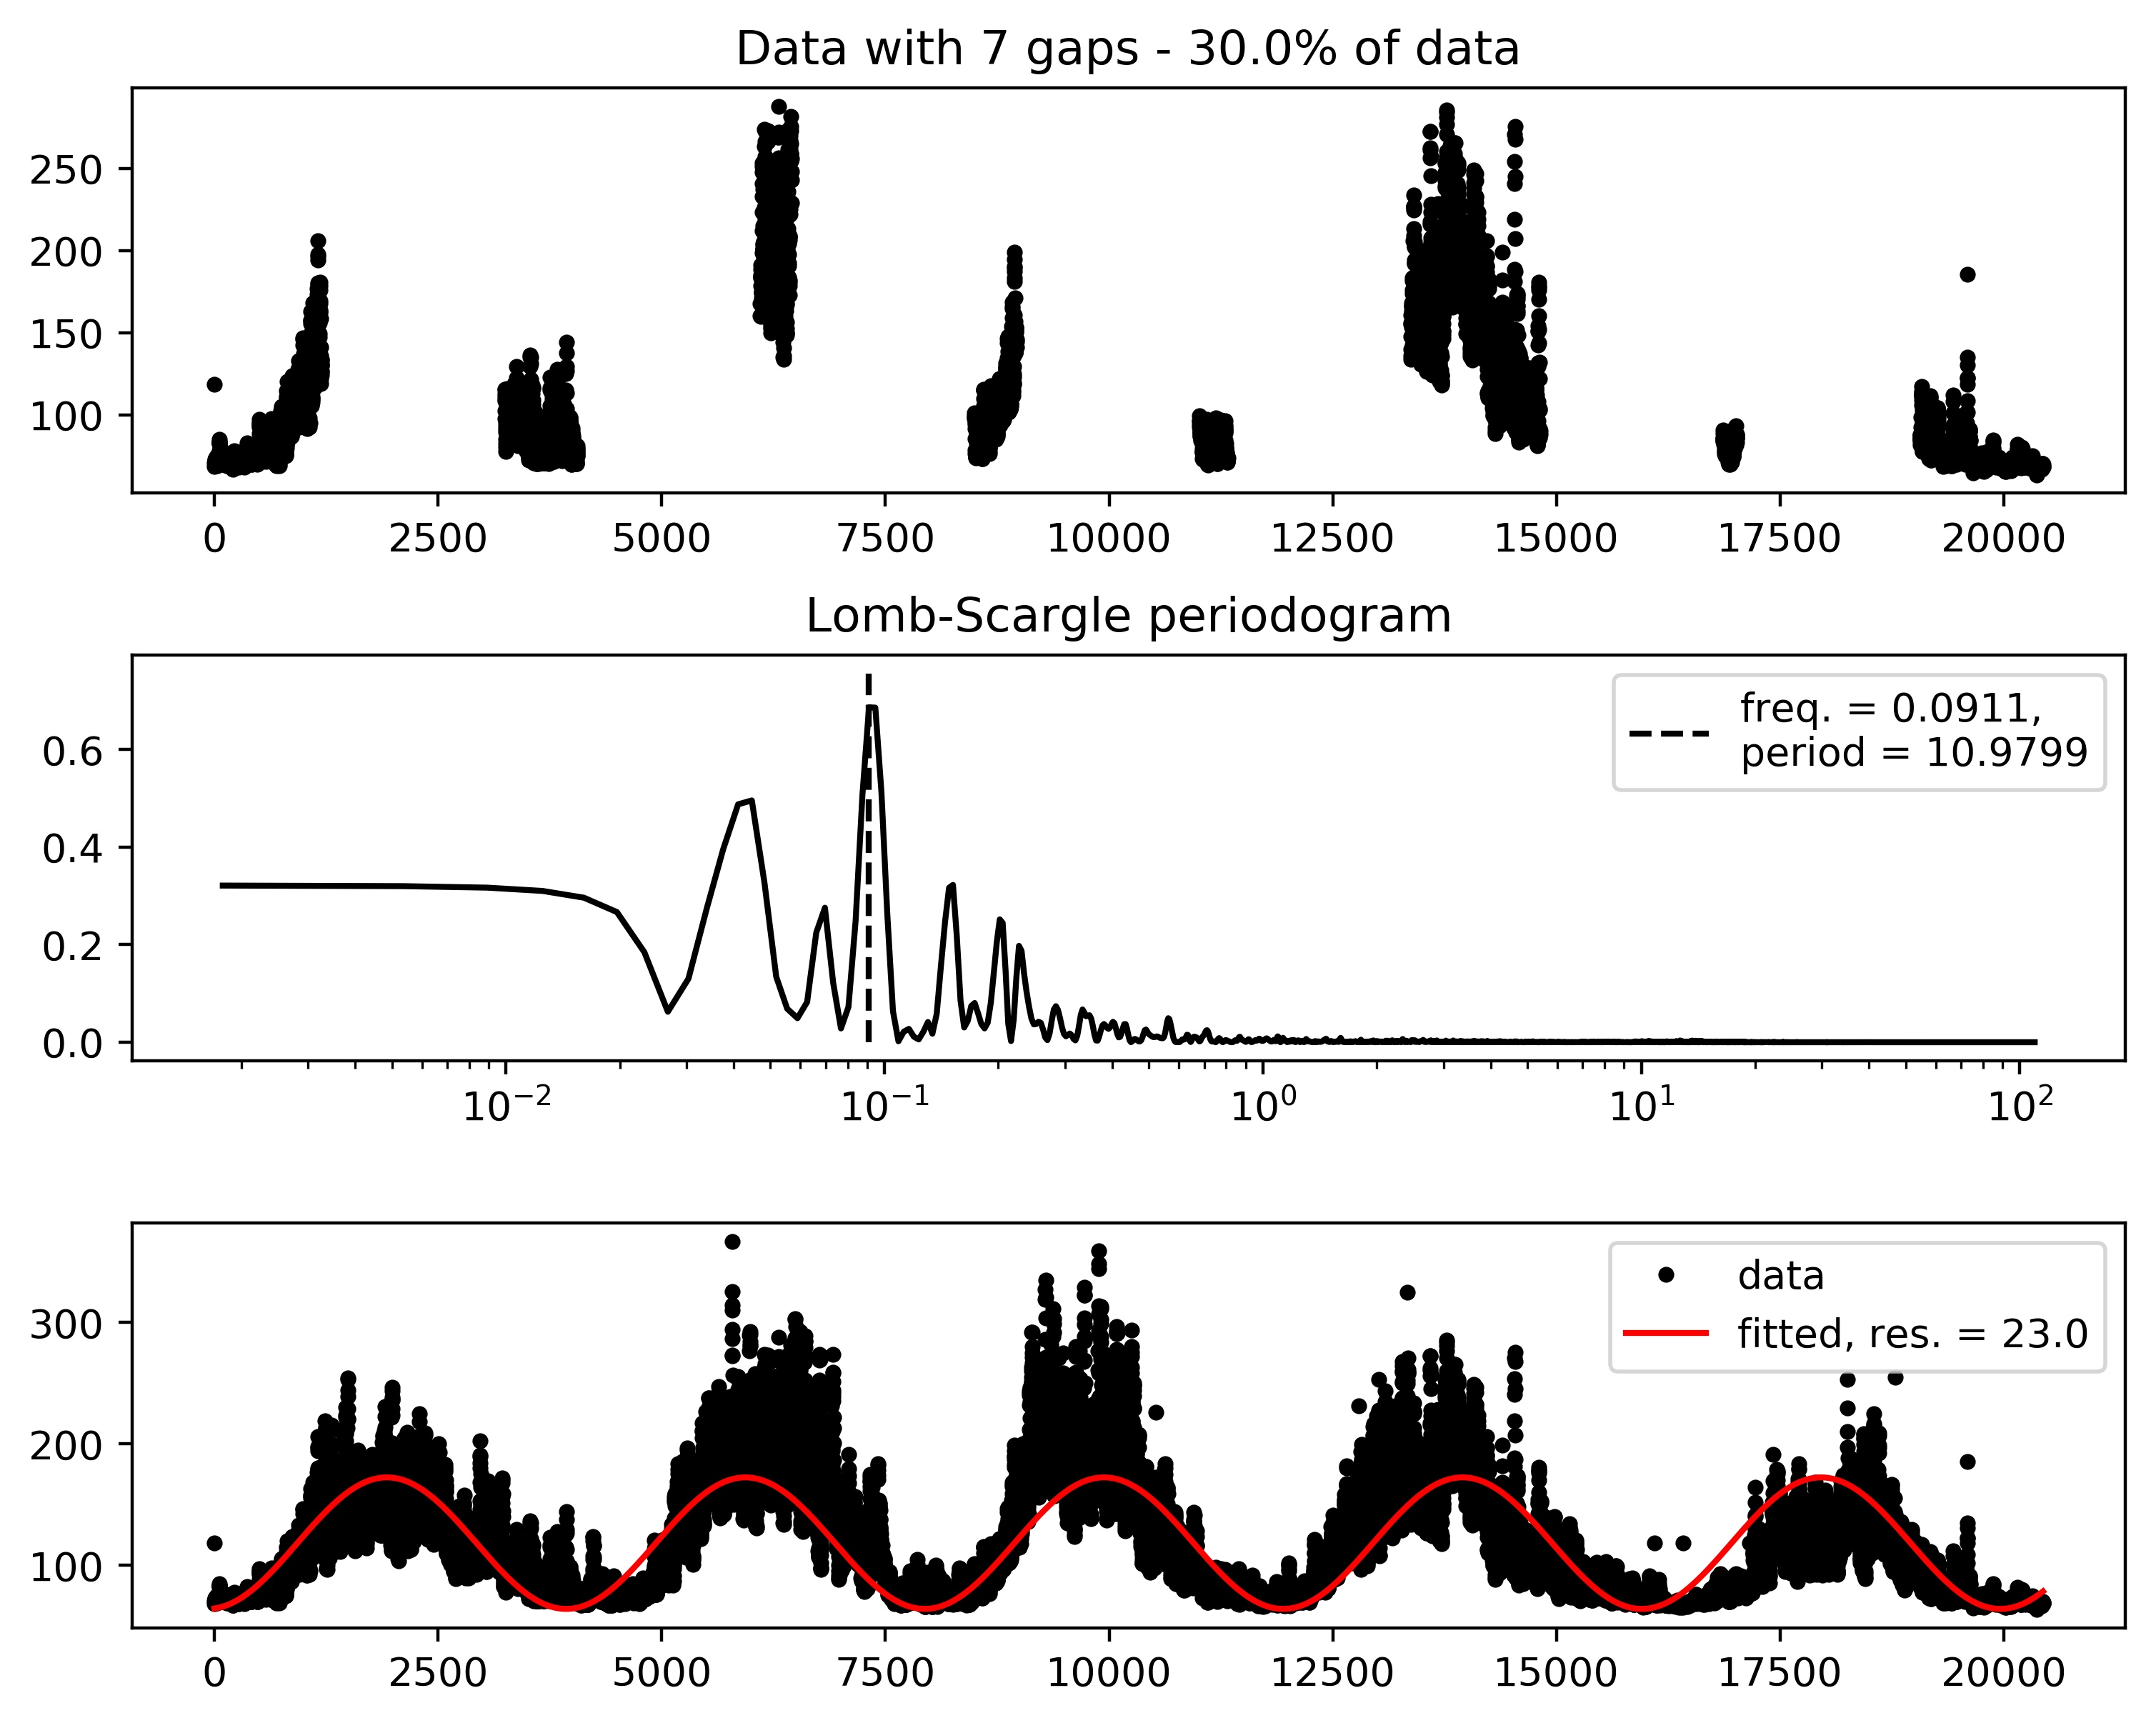
\includegraphics[scale=0.55]{../scripts/dataset1/periodograms_ny2.0_model2_Ng7.jpg}
\end{center}
\end{frame}
\begin{frame}
\frametitle{Scenario 1 - daily averages}
\begin{center}
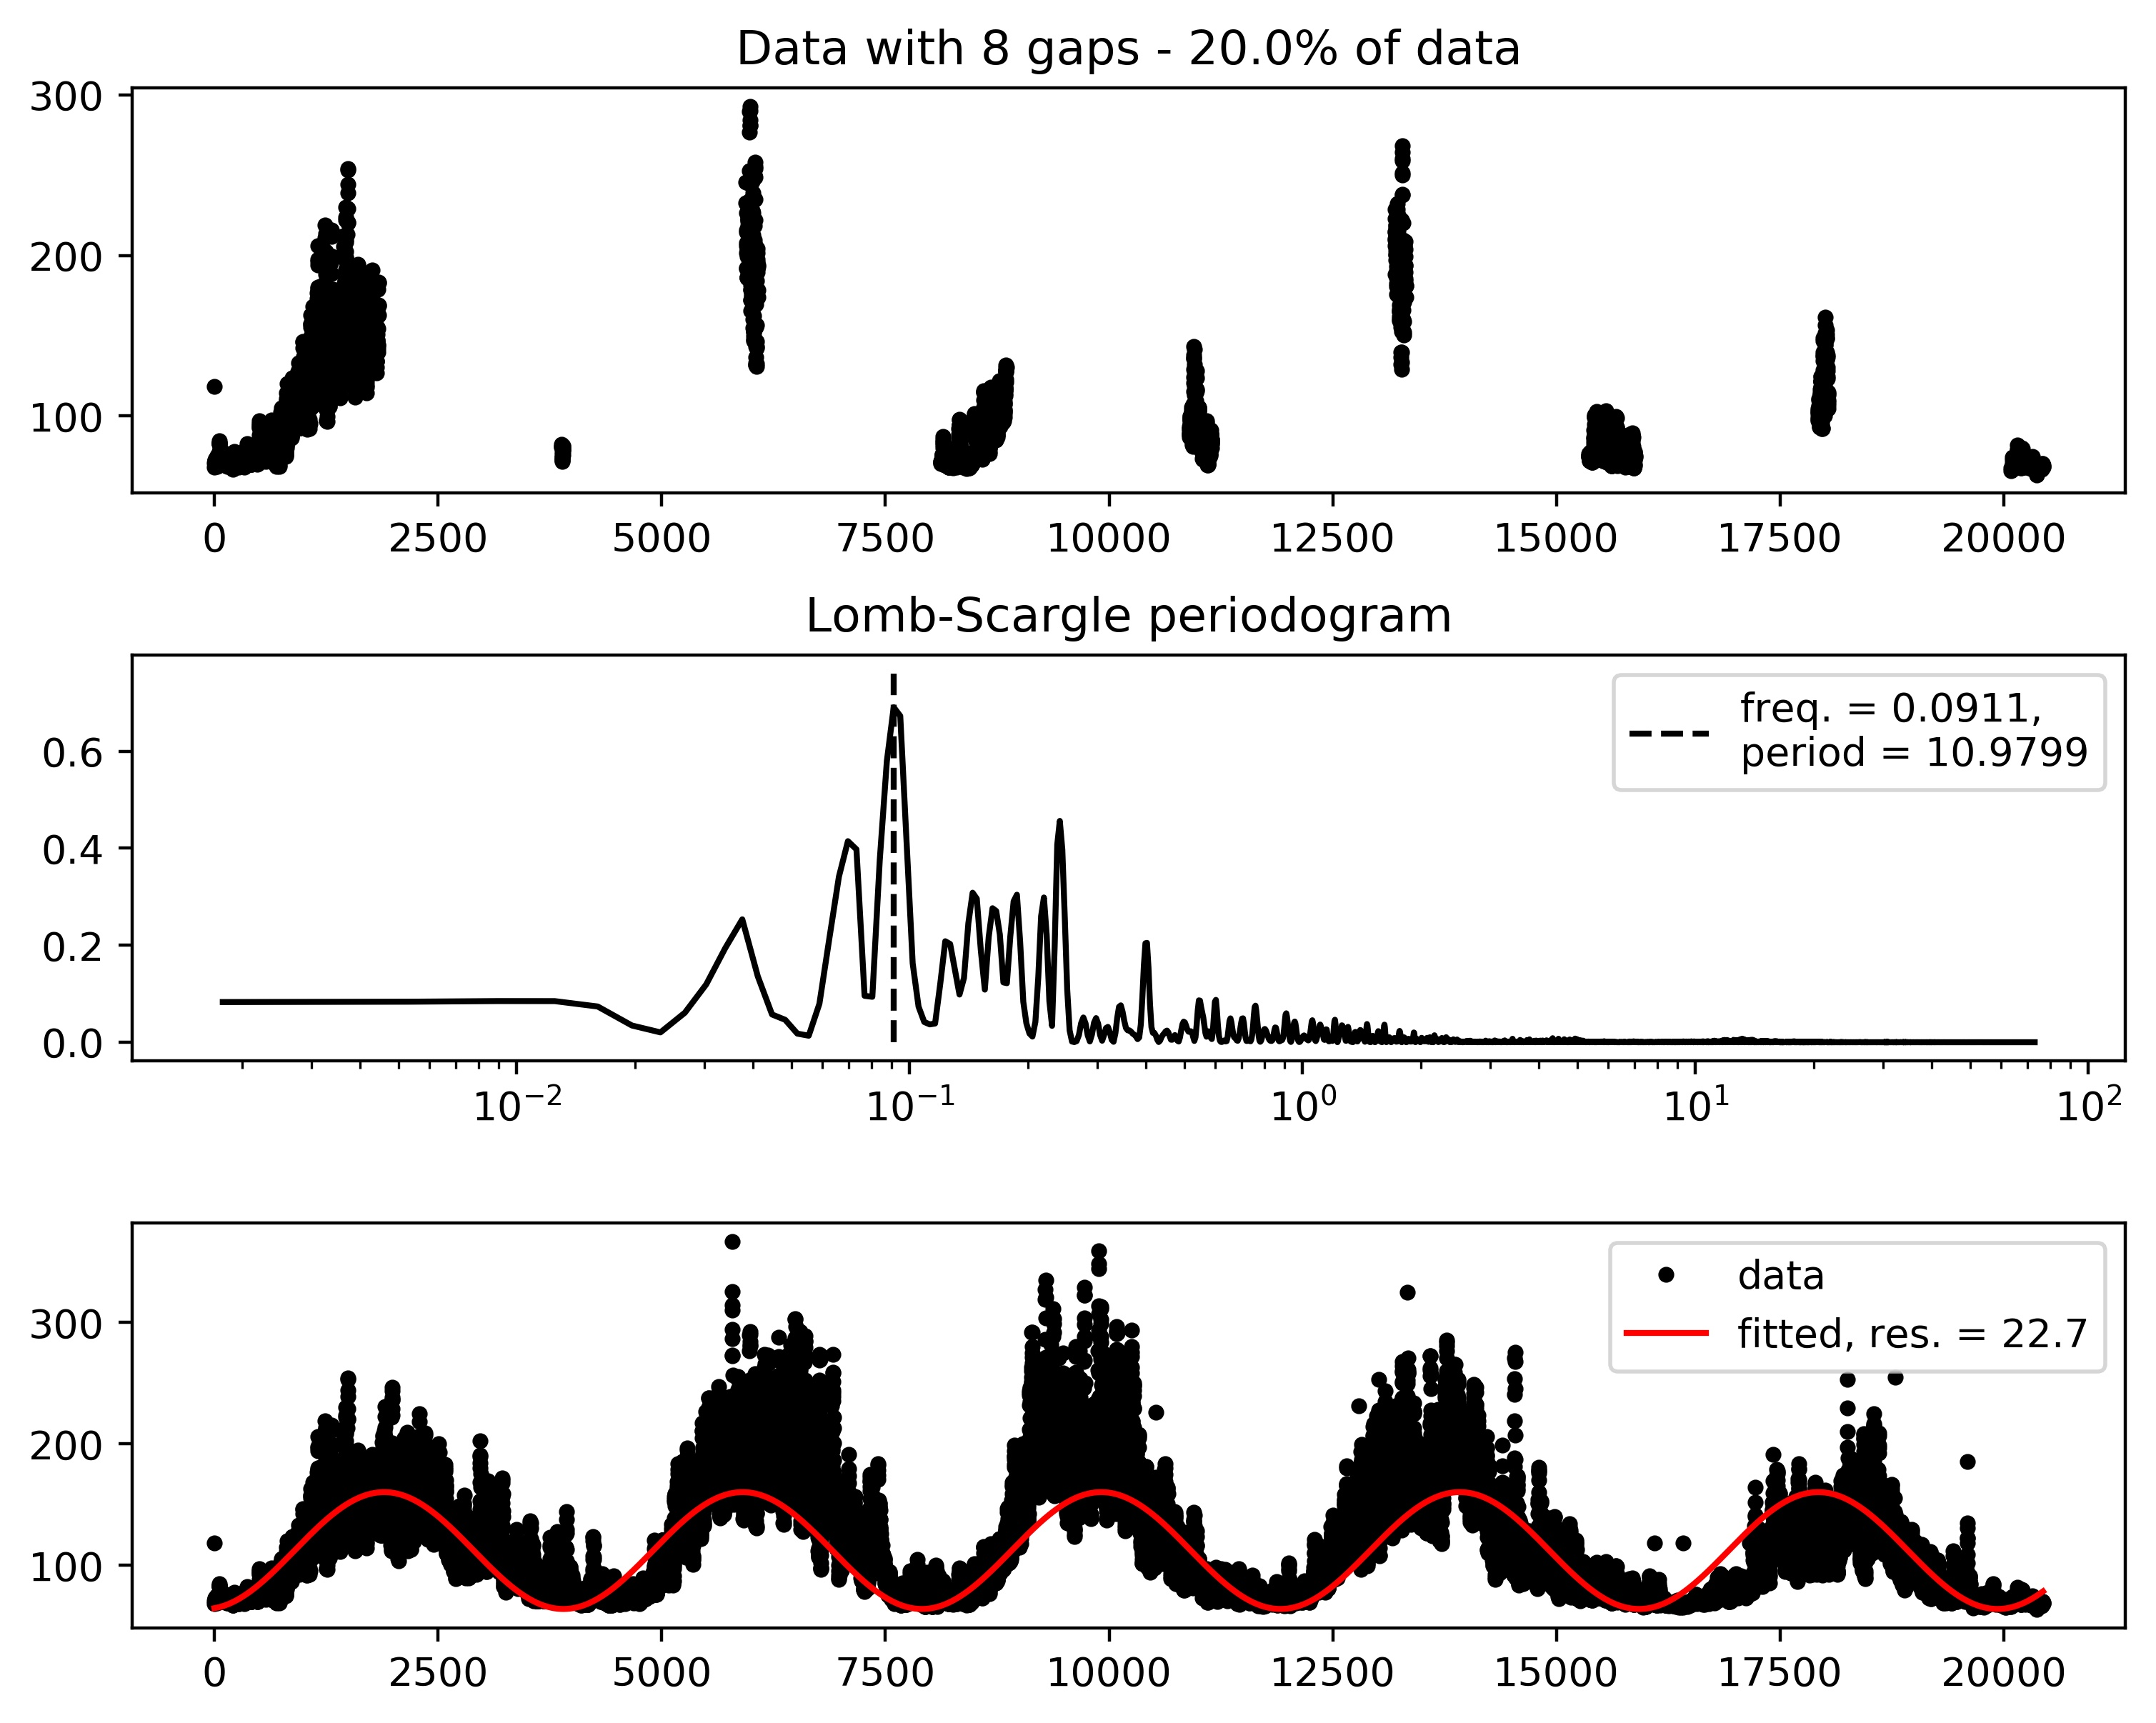
\includegraphics[scale=0.55]{../scripts/dataset1/periodograms_ny2.0_model2_Ng8.jpg}
\end{center}
\end{frame}

%%%%%%%%%%%%%%%%%%%%%%%%  FRAME  %%%%%%%%%%%%%%%%%%%%%%%%
\begin{frame}
\frametitle{Power spectrum via FFT - the usual analysis}
\begin{center}
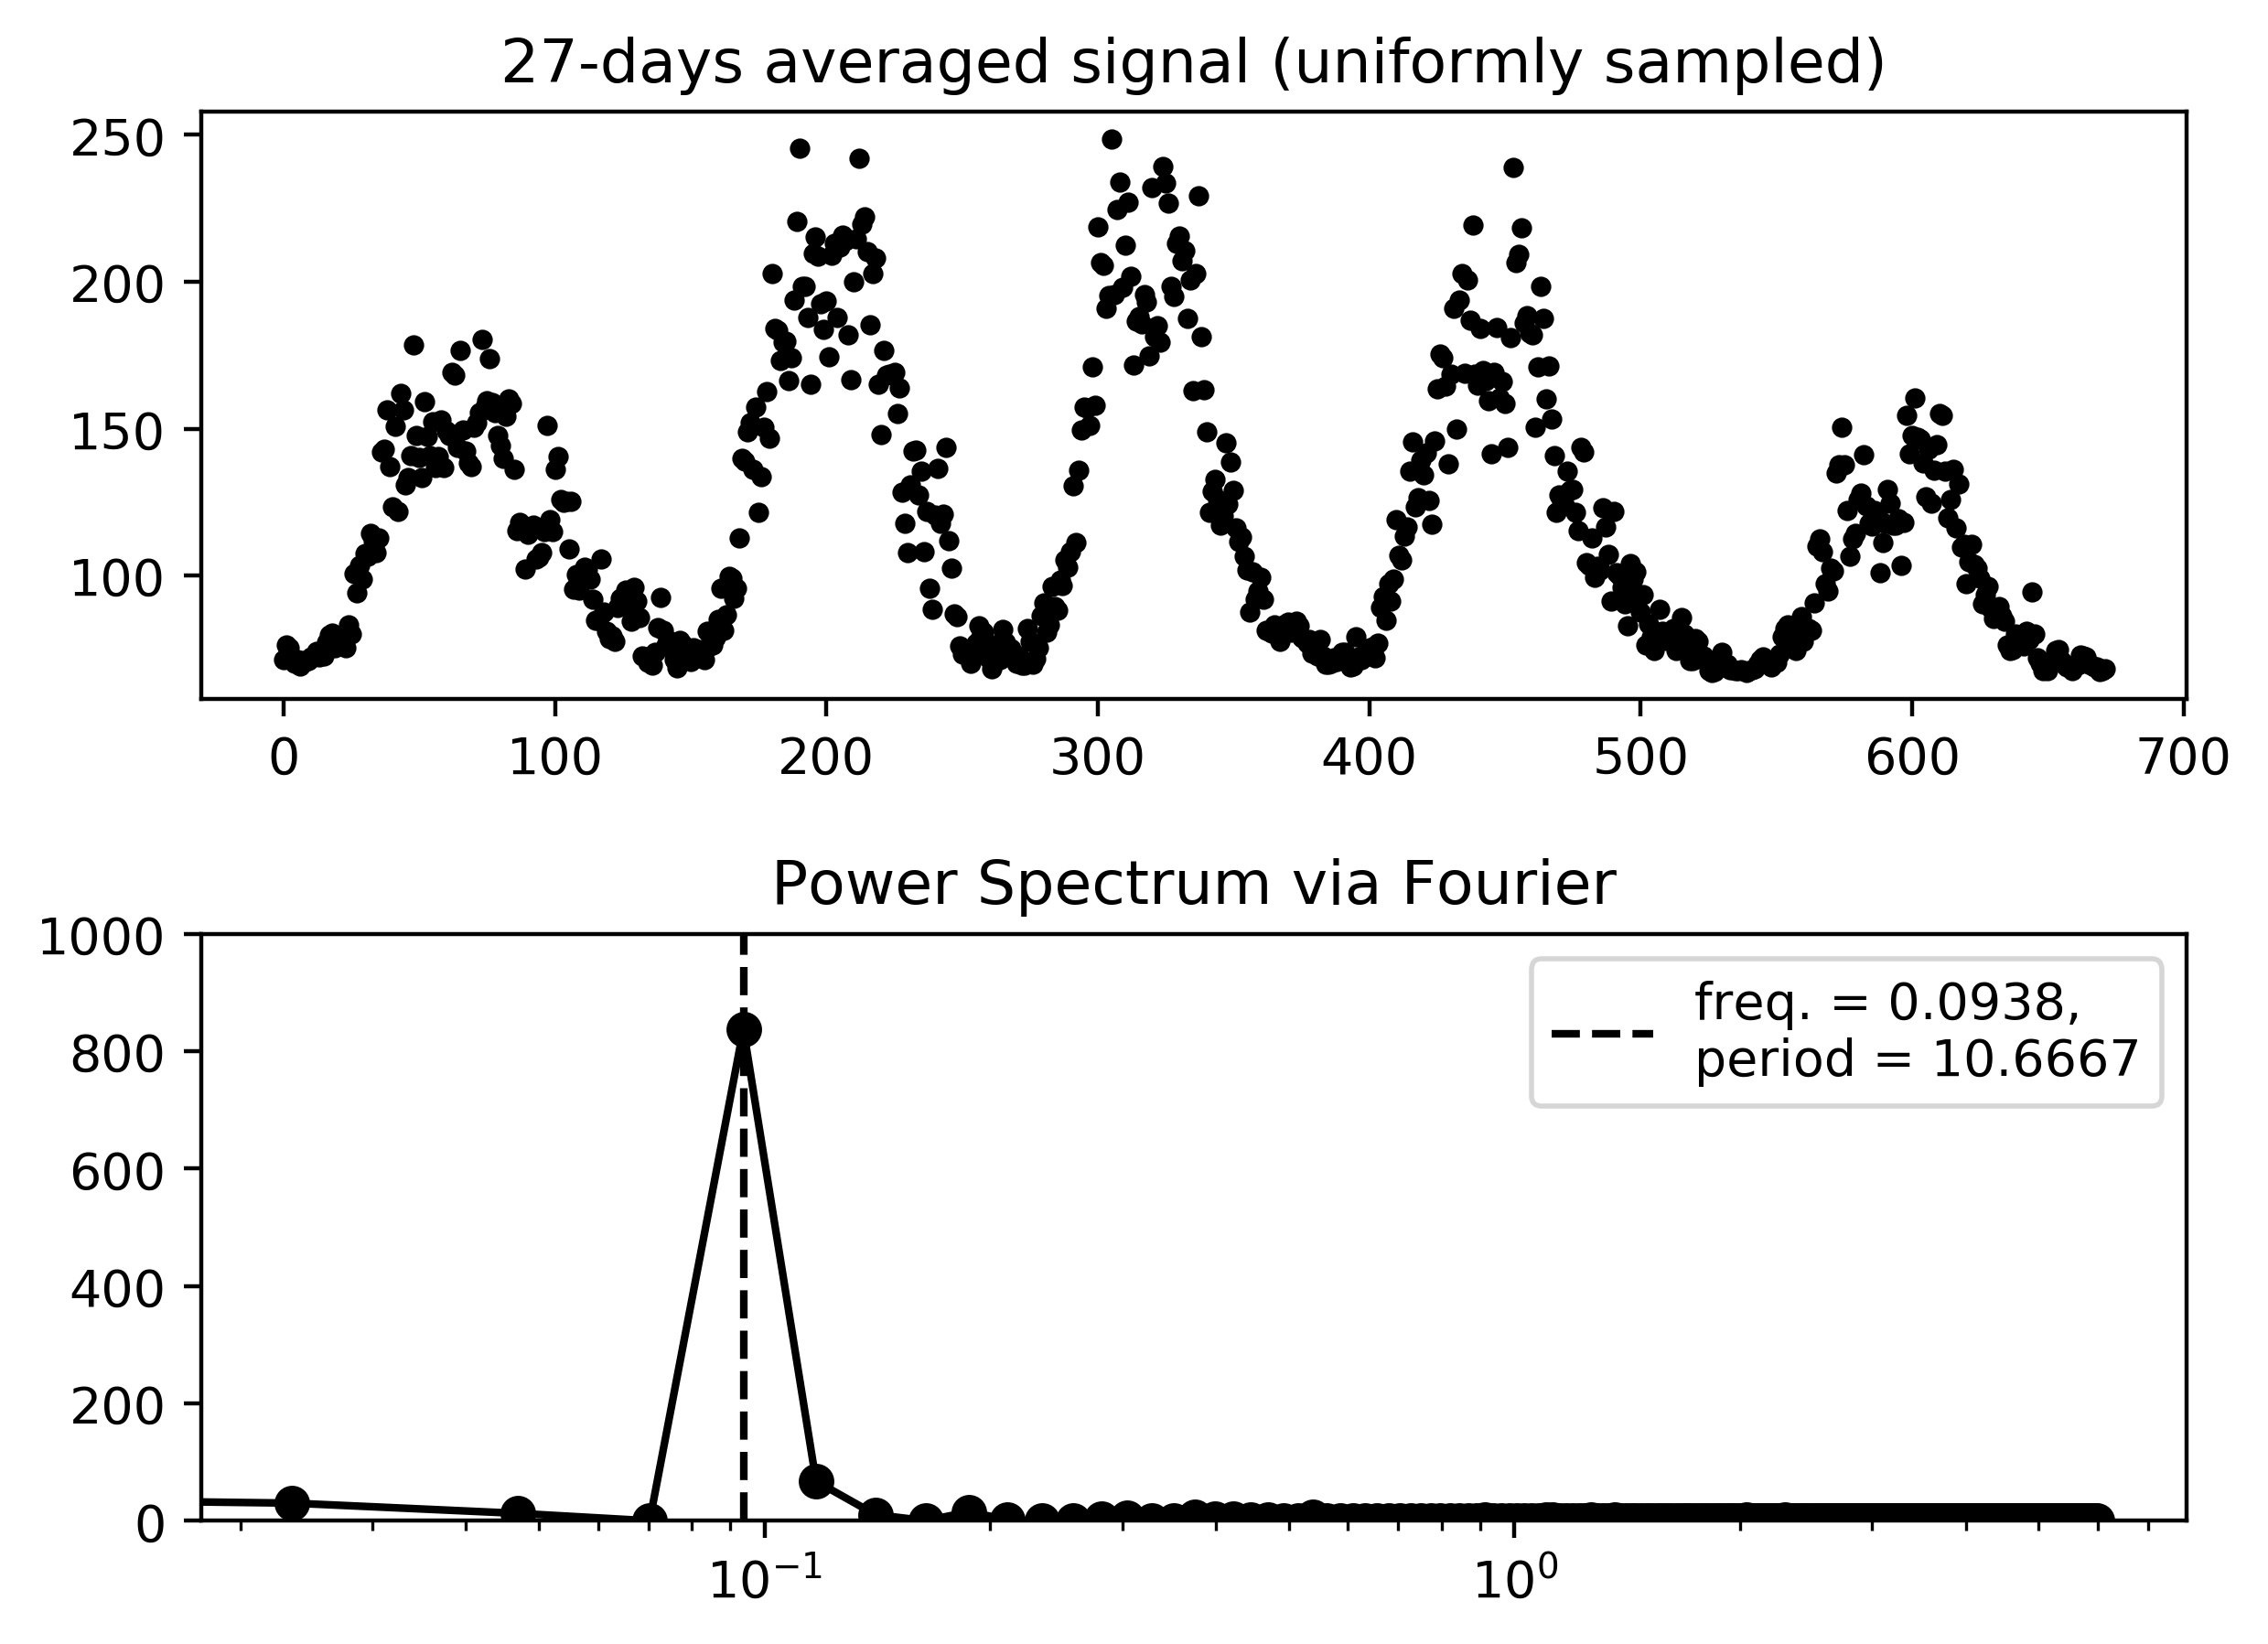
\includegraphics[scale=0.55]{Figuras/original_12.jpg}
\end{center}
\end{frame}

%%%%%%%%%%%%%%%%%%%%%%%%  FRAME  %%%%%%%%%%%%%%%%%%%%%%%%
\begin{frame}
\frametitle{Scenario 1 - 27-day averages}
\begin{center}
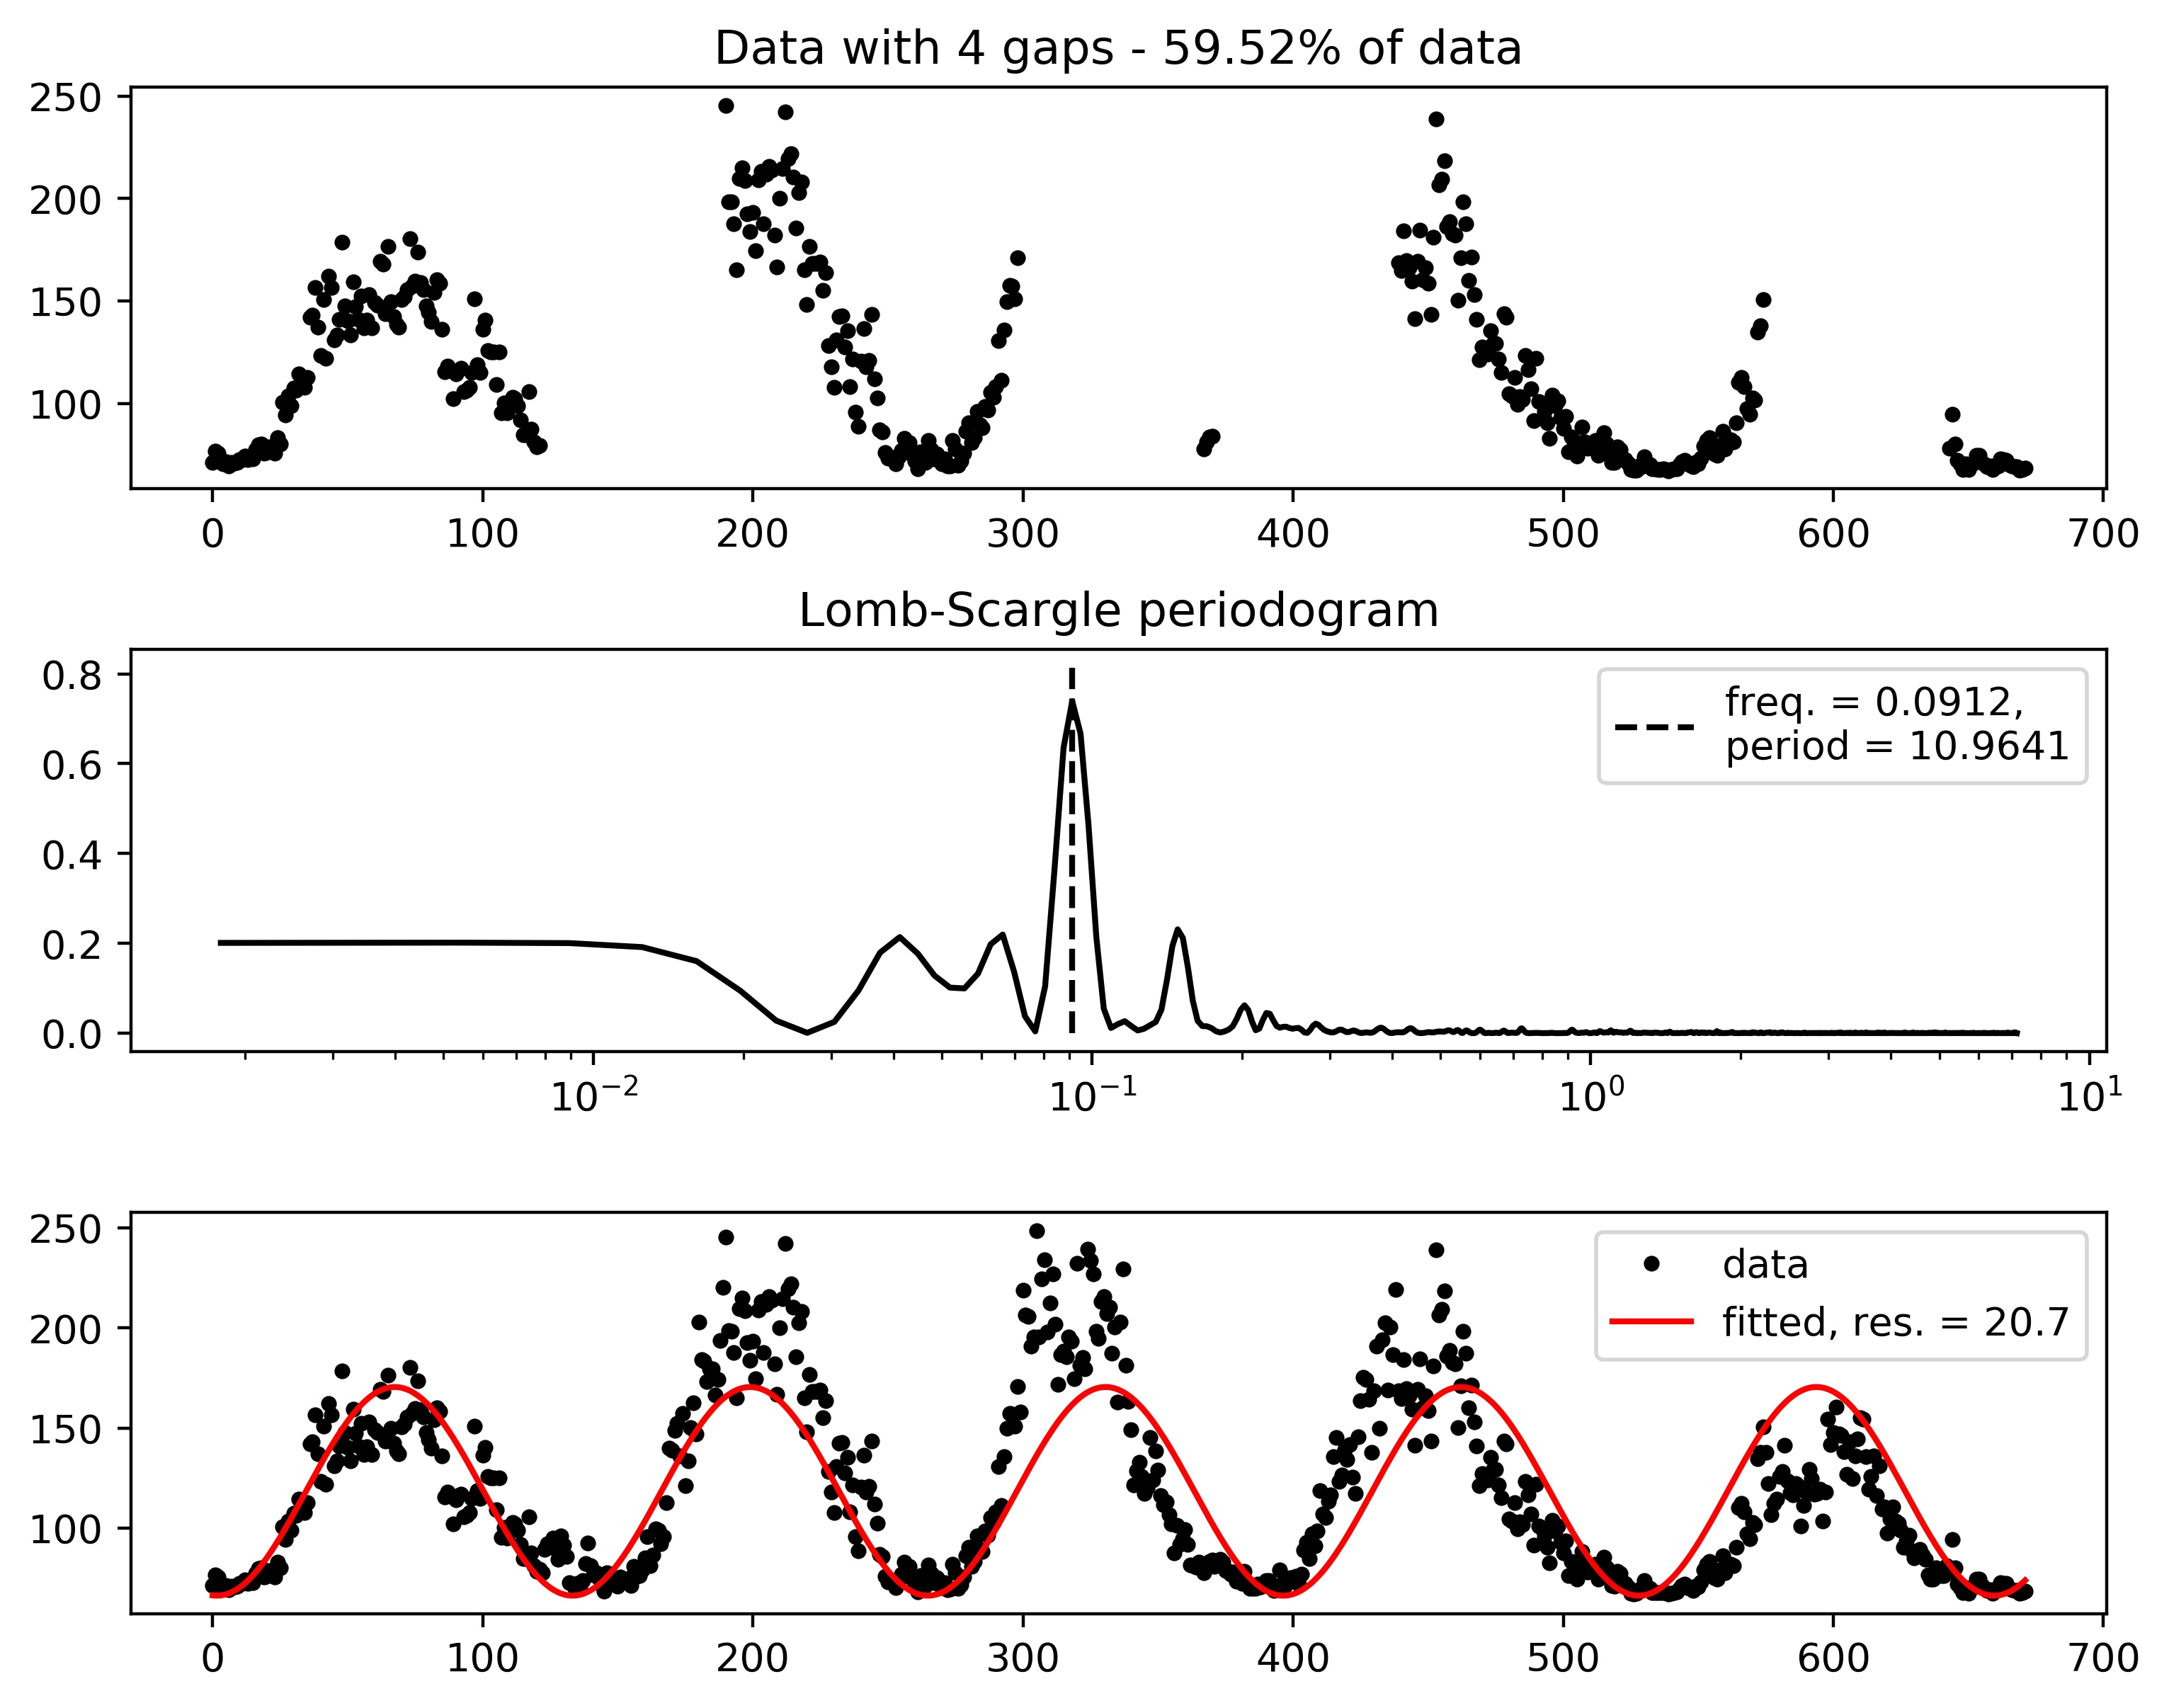
\includegraphics[scale=0.55]{../scripts/dataset2/periodograms_ny2.0_model2_Ng4.jpg}
\end{center}
\end{frame}
\begin{frame}
\frametitle{Scenario 1 - 27-day averages}
\begin{center}
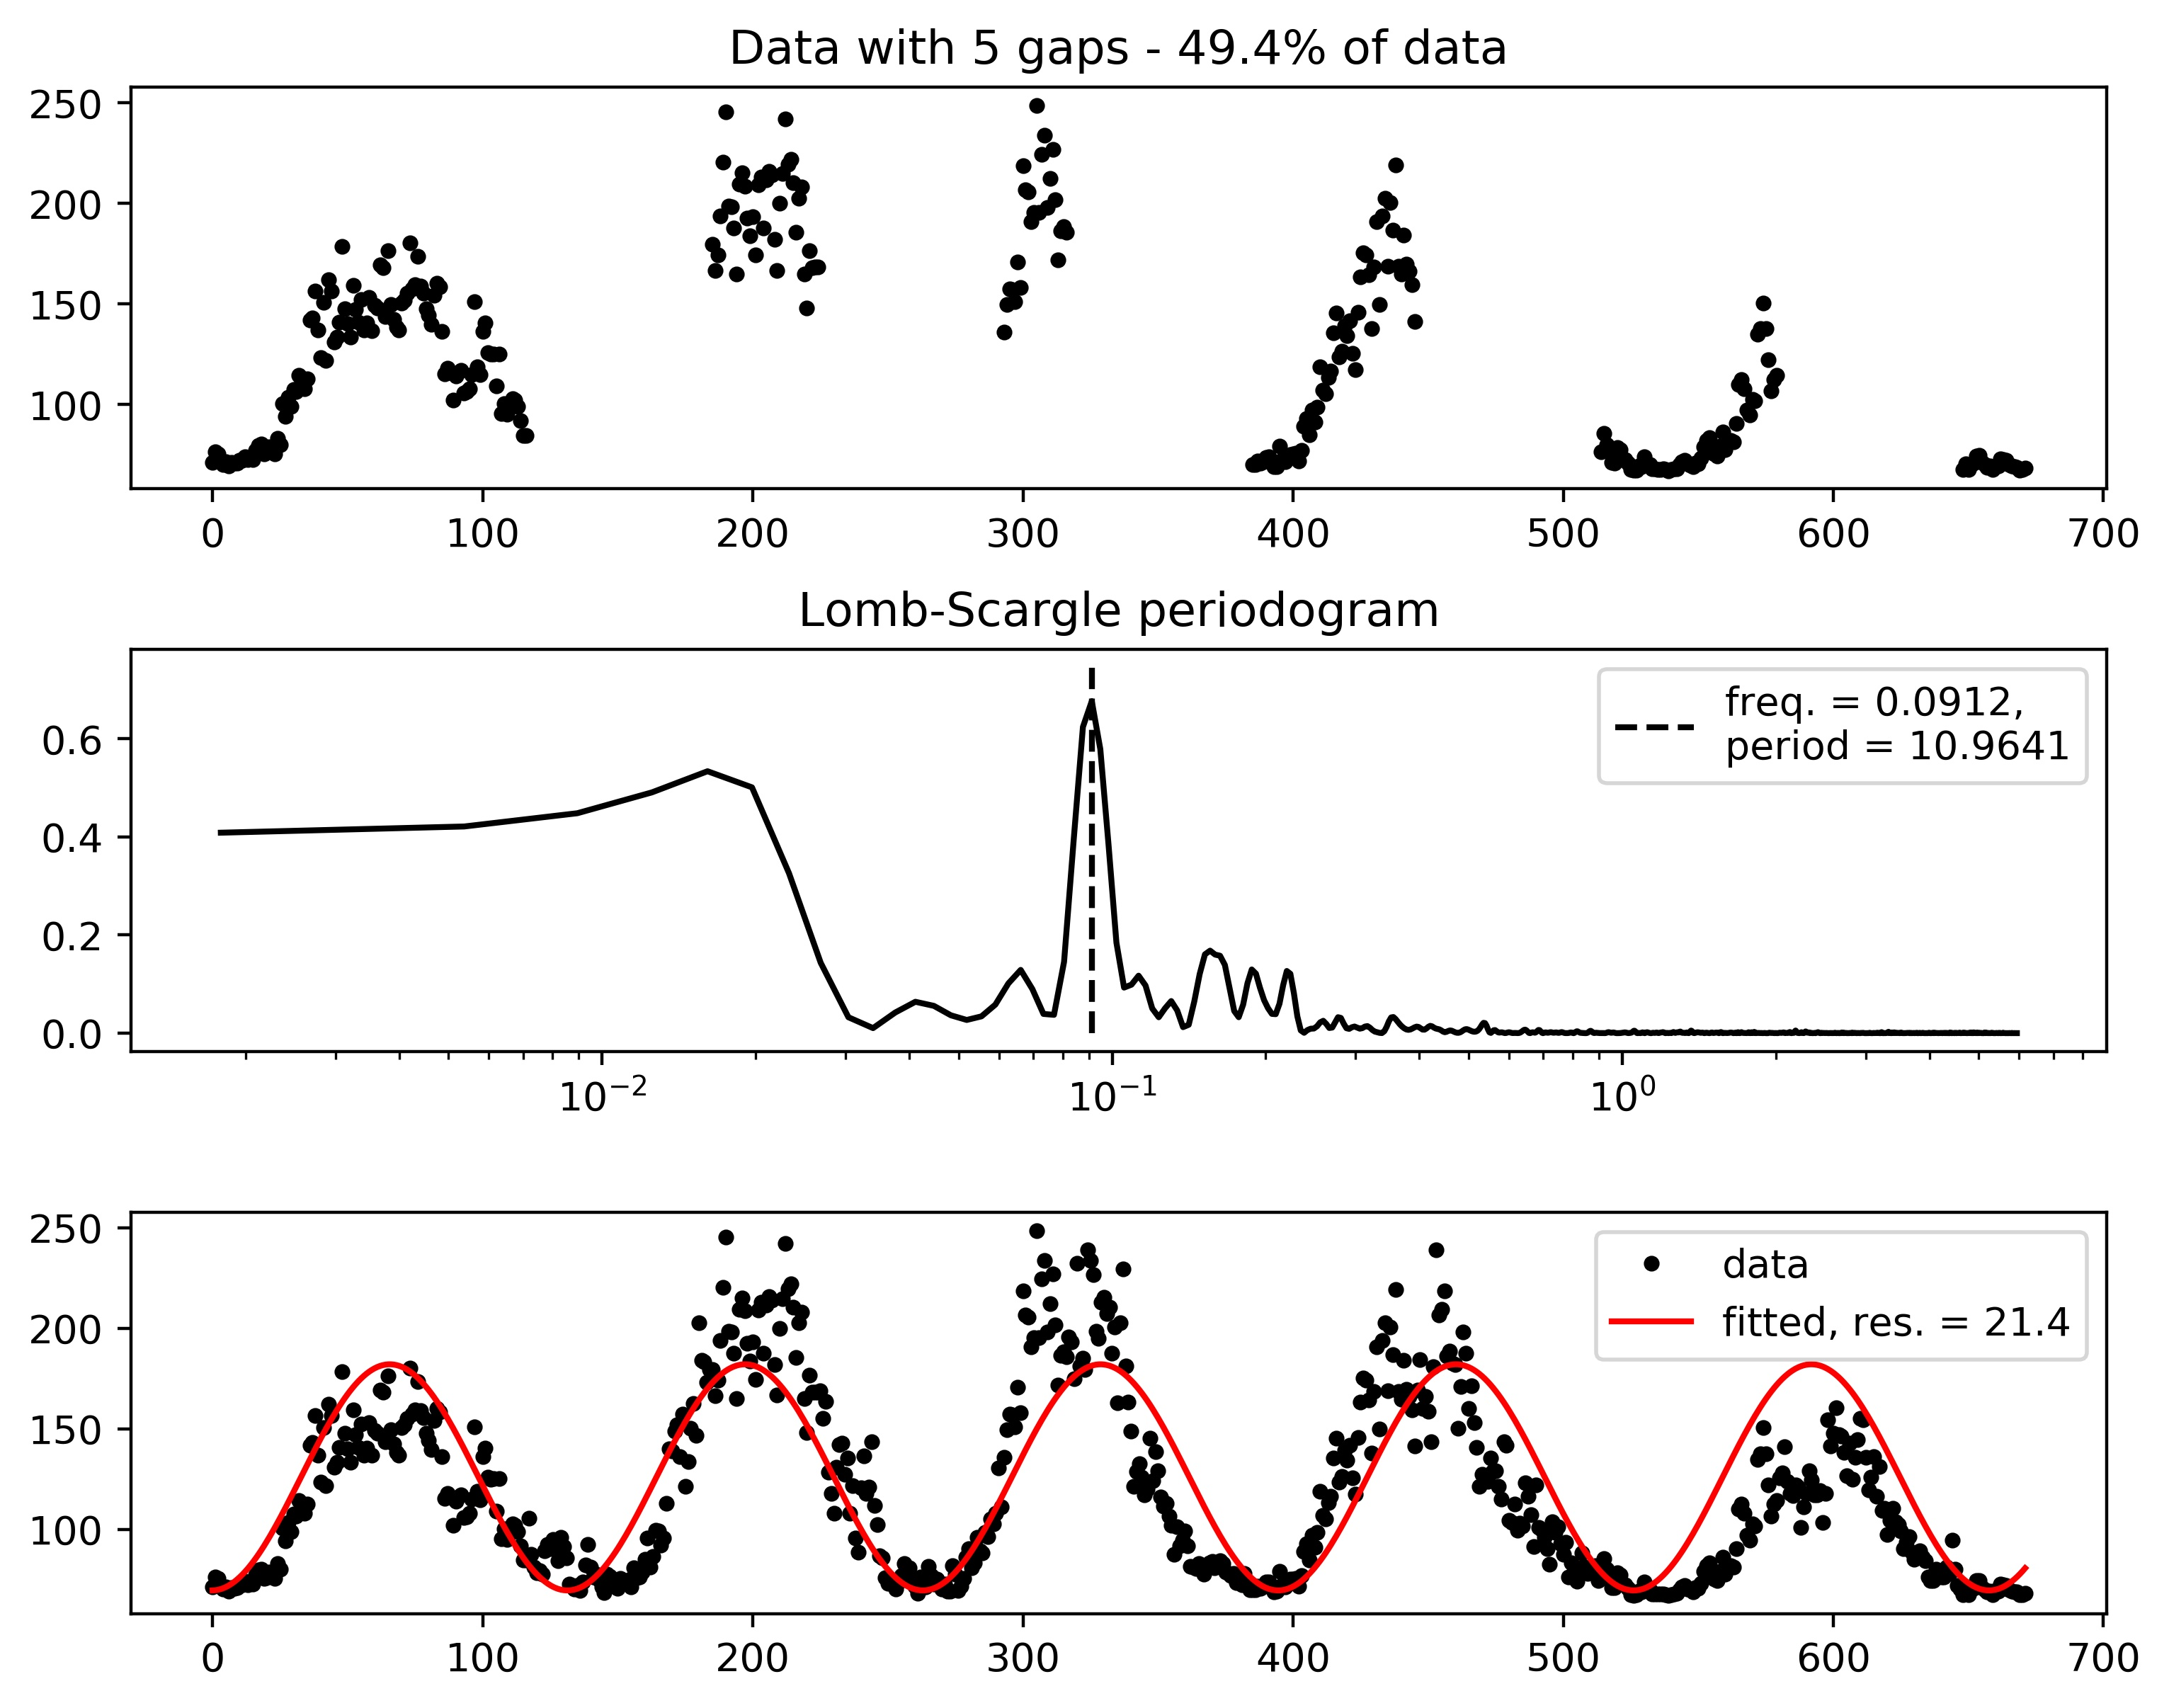
\includegraphics[scale=0.55]{../scripts/dataset2/periodograms_ny2.0_model2_Ng5.jpg}
\end{center}
\end{frame}
\begin{frame}
\frametitle{Scenario 1 - 27-day averages}
\begin{center}
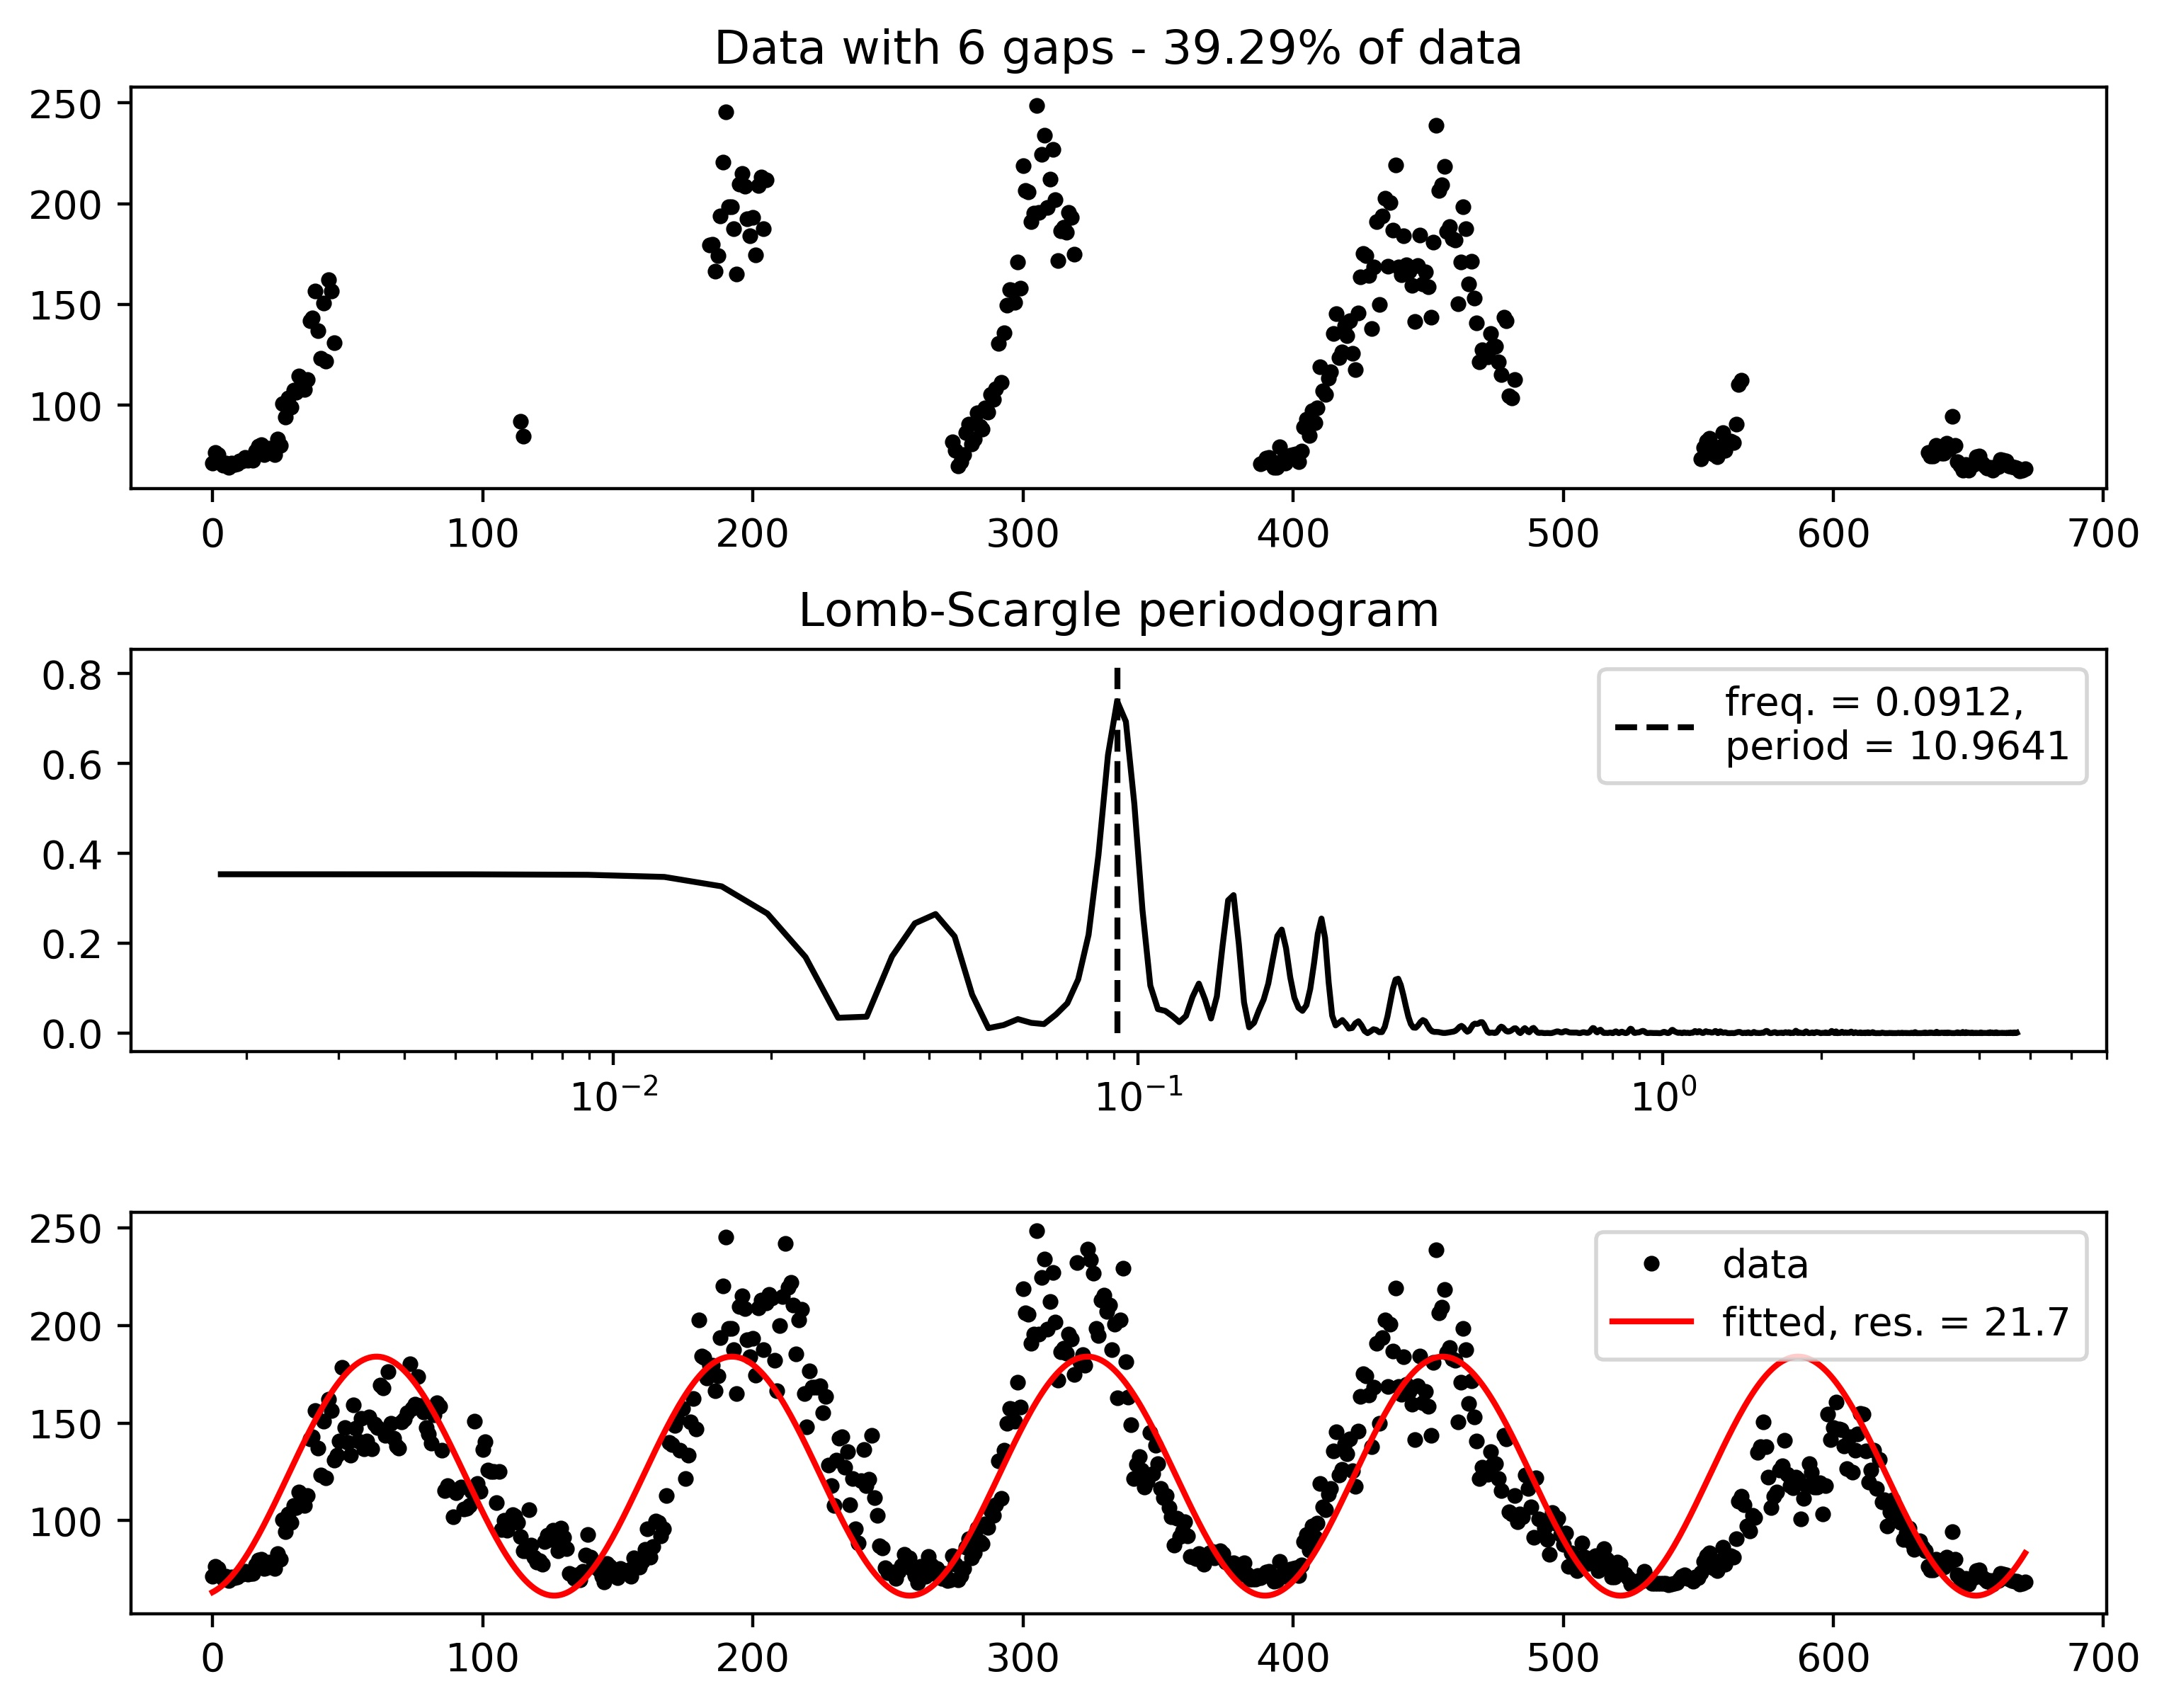
\includegraphics[scale=0.55]{../scripts/dataset2/periodograms_ny2.0_model2_Ng6.jpg}
\end{center}
\end{frame}
\begin{frame}
\frametitle{Scenario 1 - 27-day averages}
\begin{center}
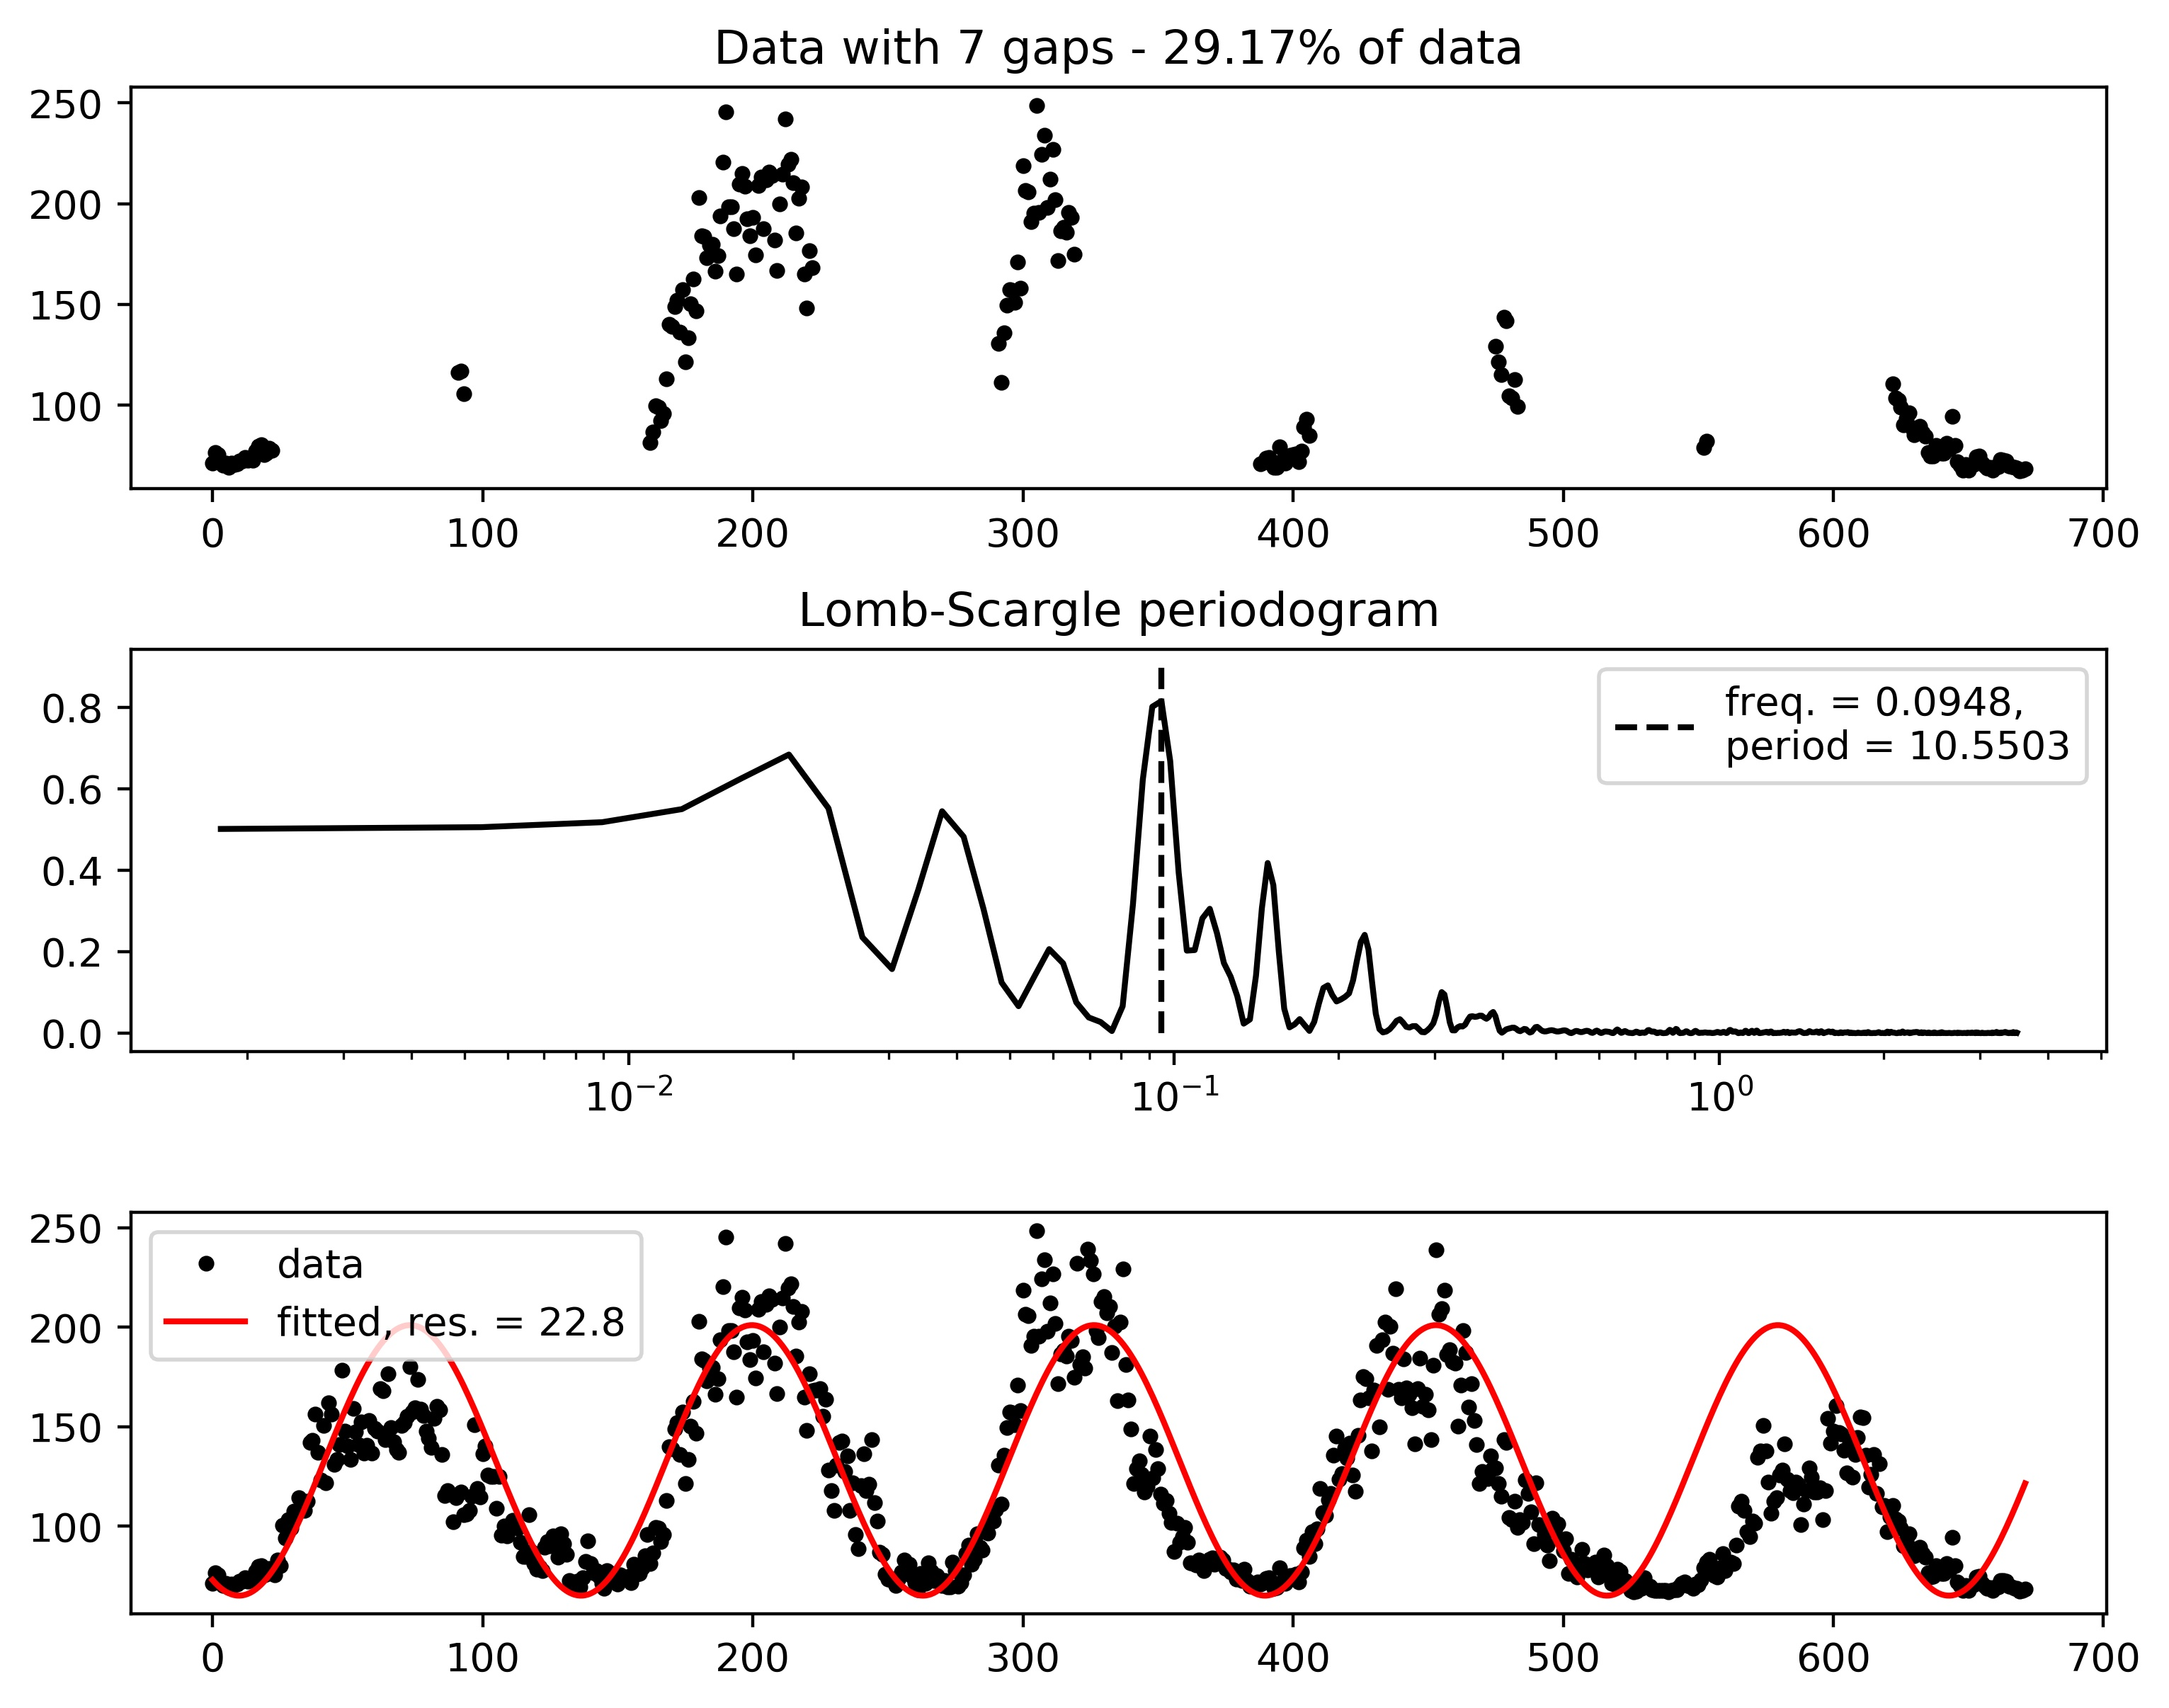
\includegraphics[scale=0.55]{../scripts/dataset2/periodograms_ny2.0_model2_Ng7.jpg}
\end{center}
\end{frame}
\begin{frame}
\frametitle{Scenario 1 - 27-day averages}
\begin{center}
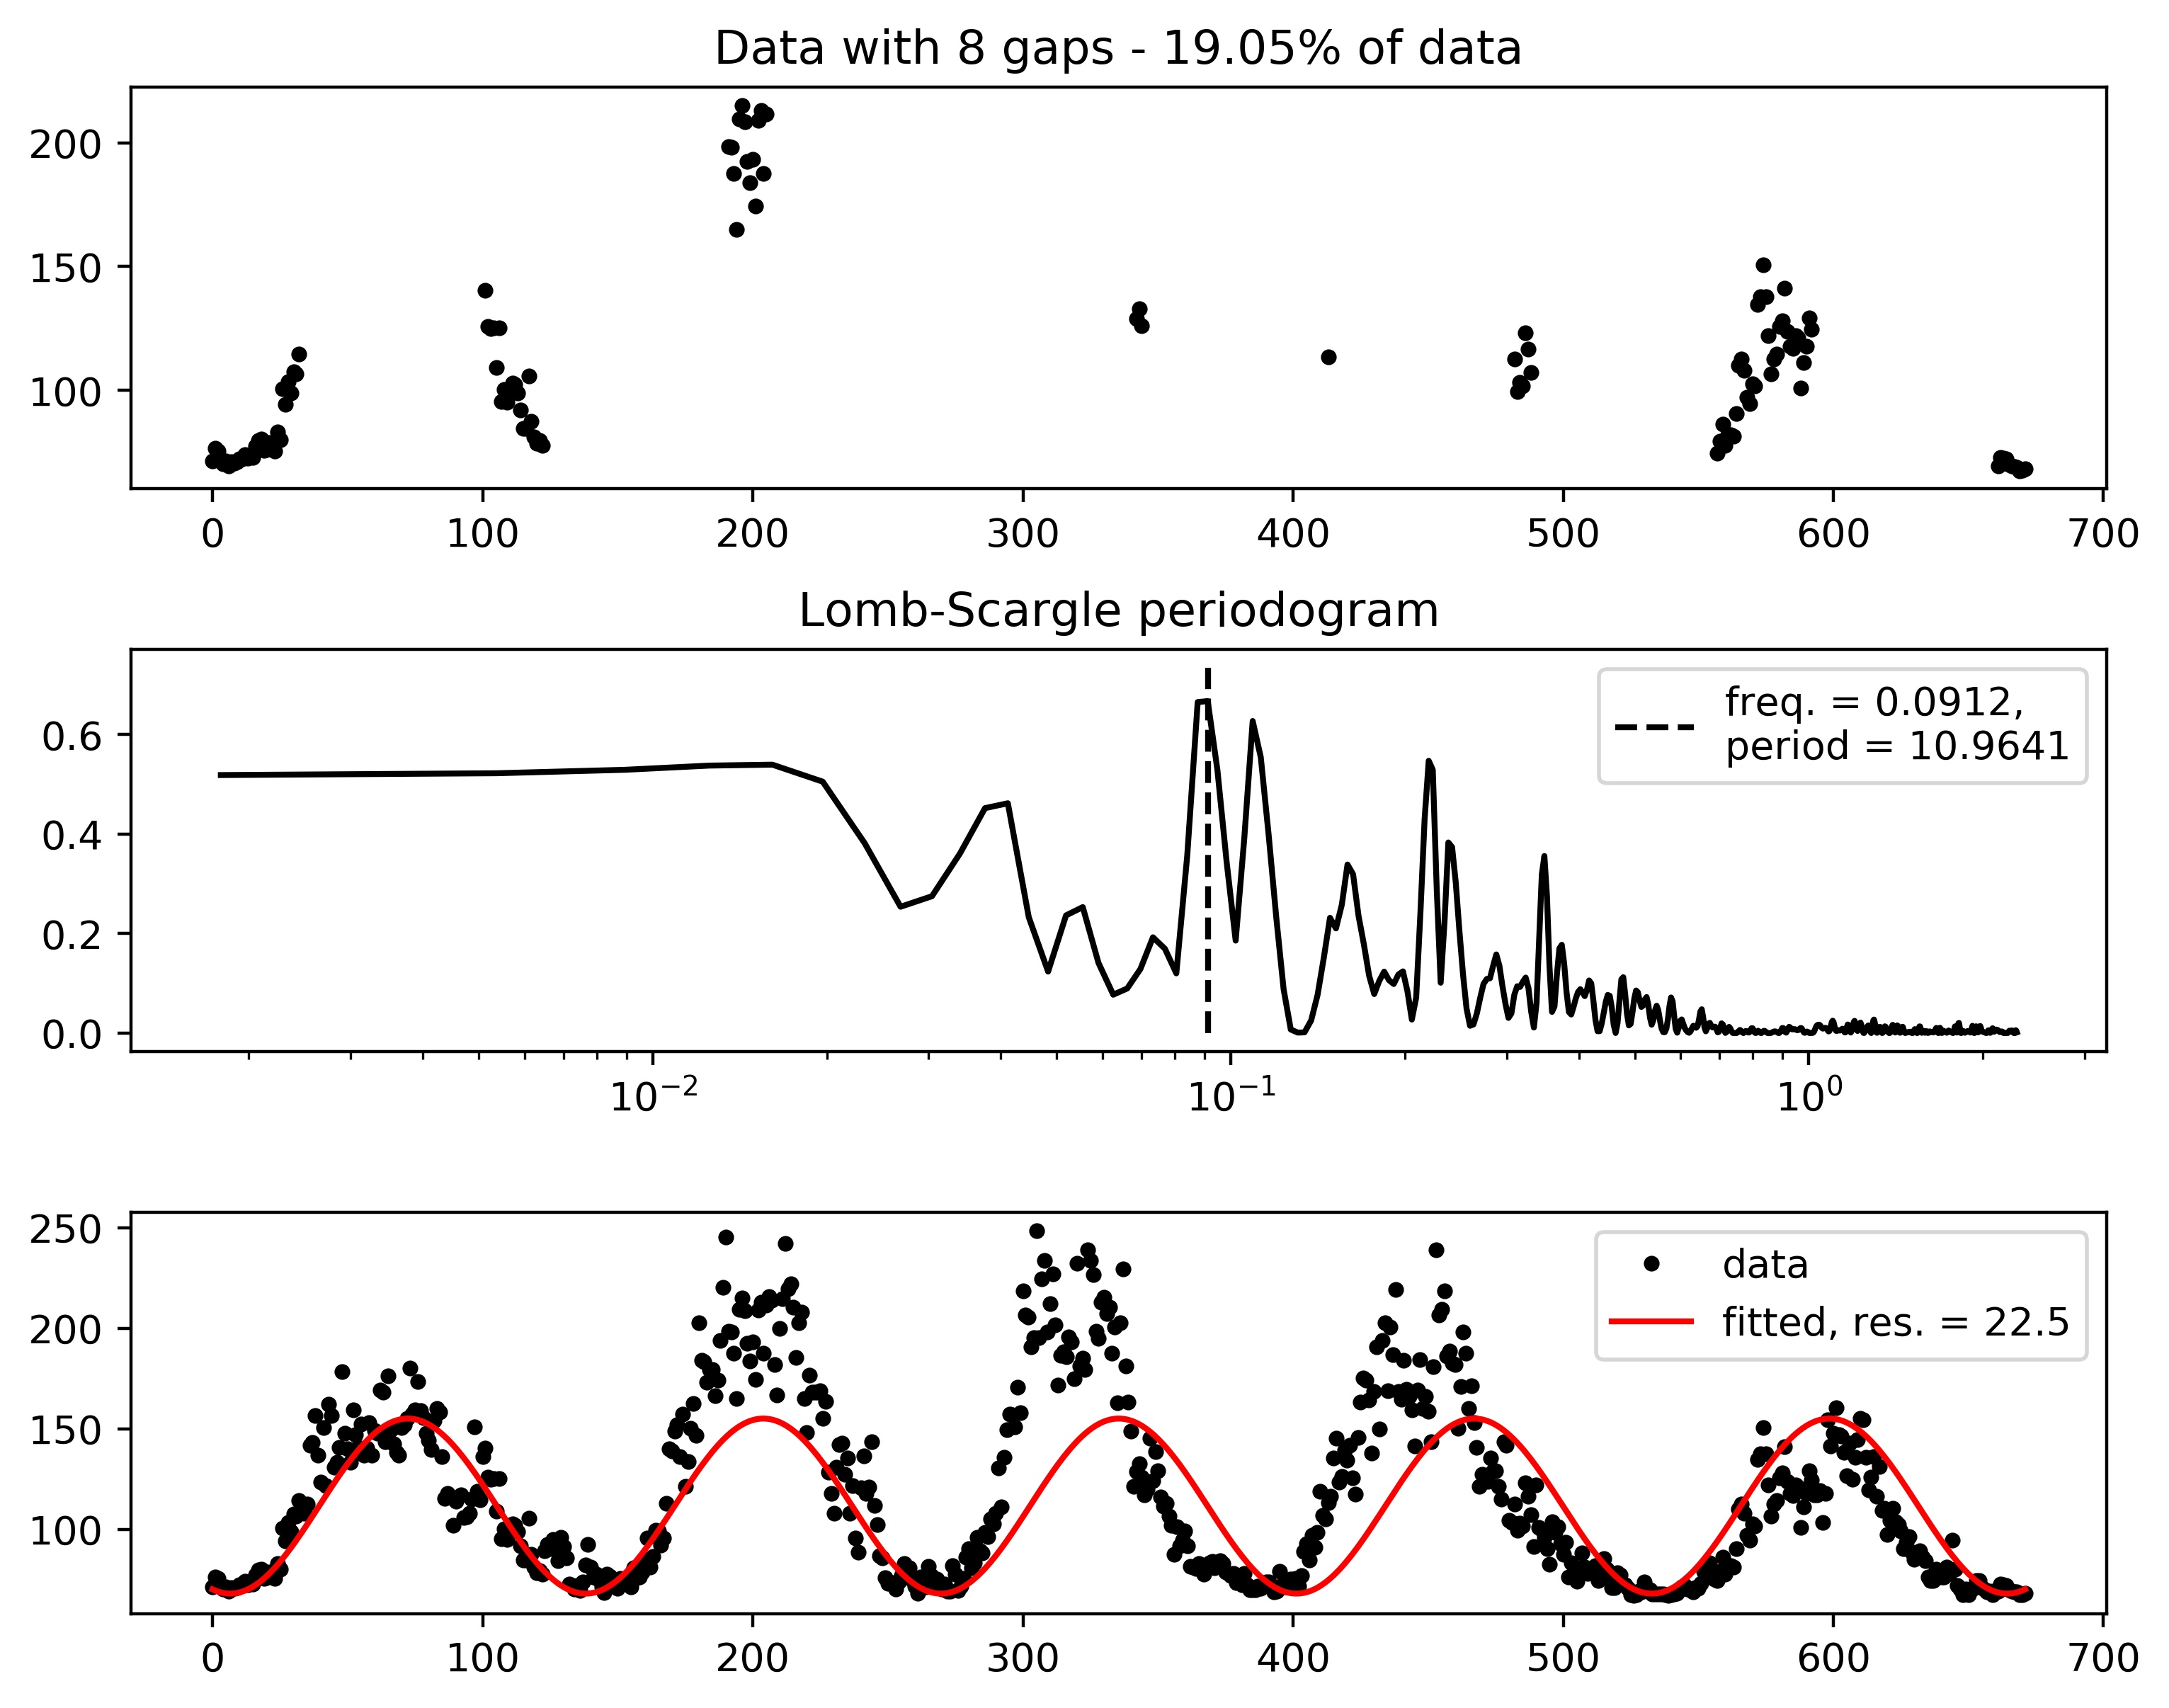
\includegraphics[scale=0.55]{../scripts/dataset2/periodograms_ny2.0_model2_Ng8.jpg}
\end{center}
\end{frame}

%%%%%%%%%%%%%%%%%%%%%%%%  FRAME  %%%%%%%%%%%%%%%%%%%%%%%%
\begin{frame}
\frametitle{Power spectrum via FFT - the usual analysis}
\begin{center}
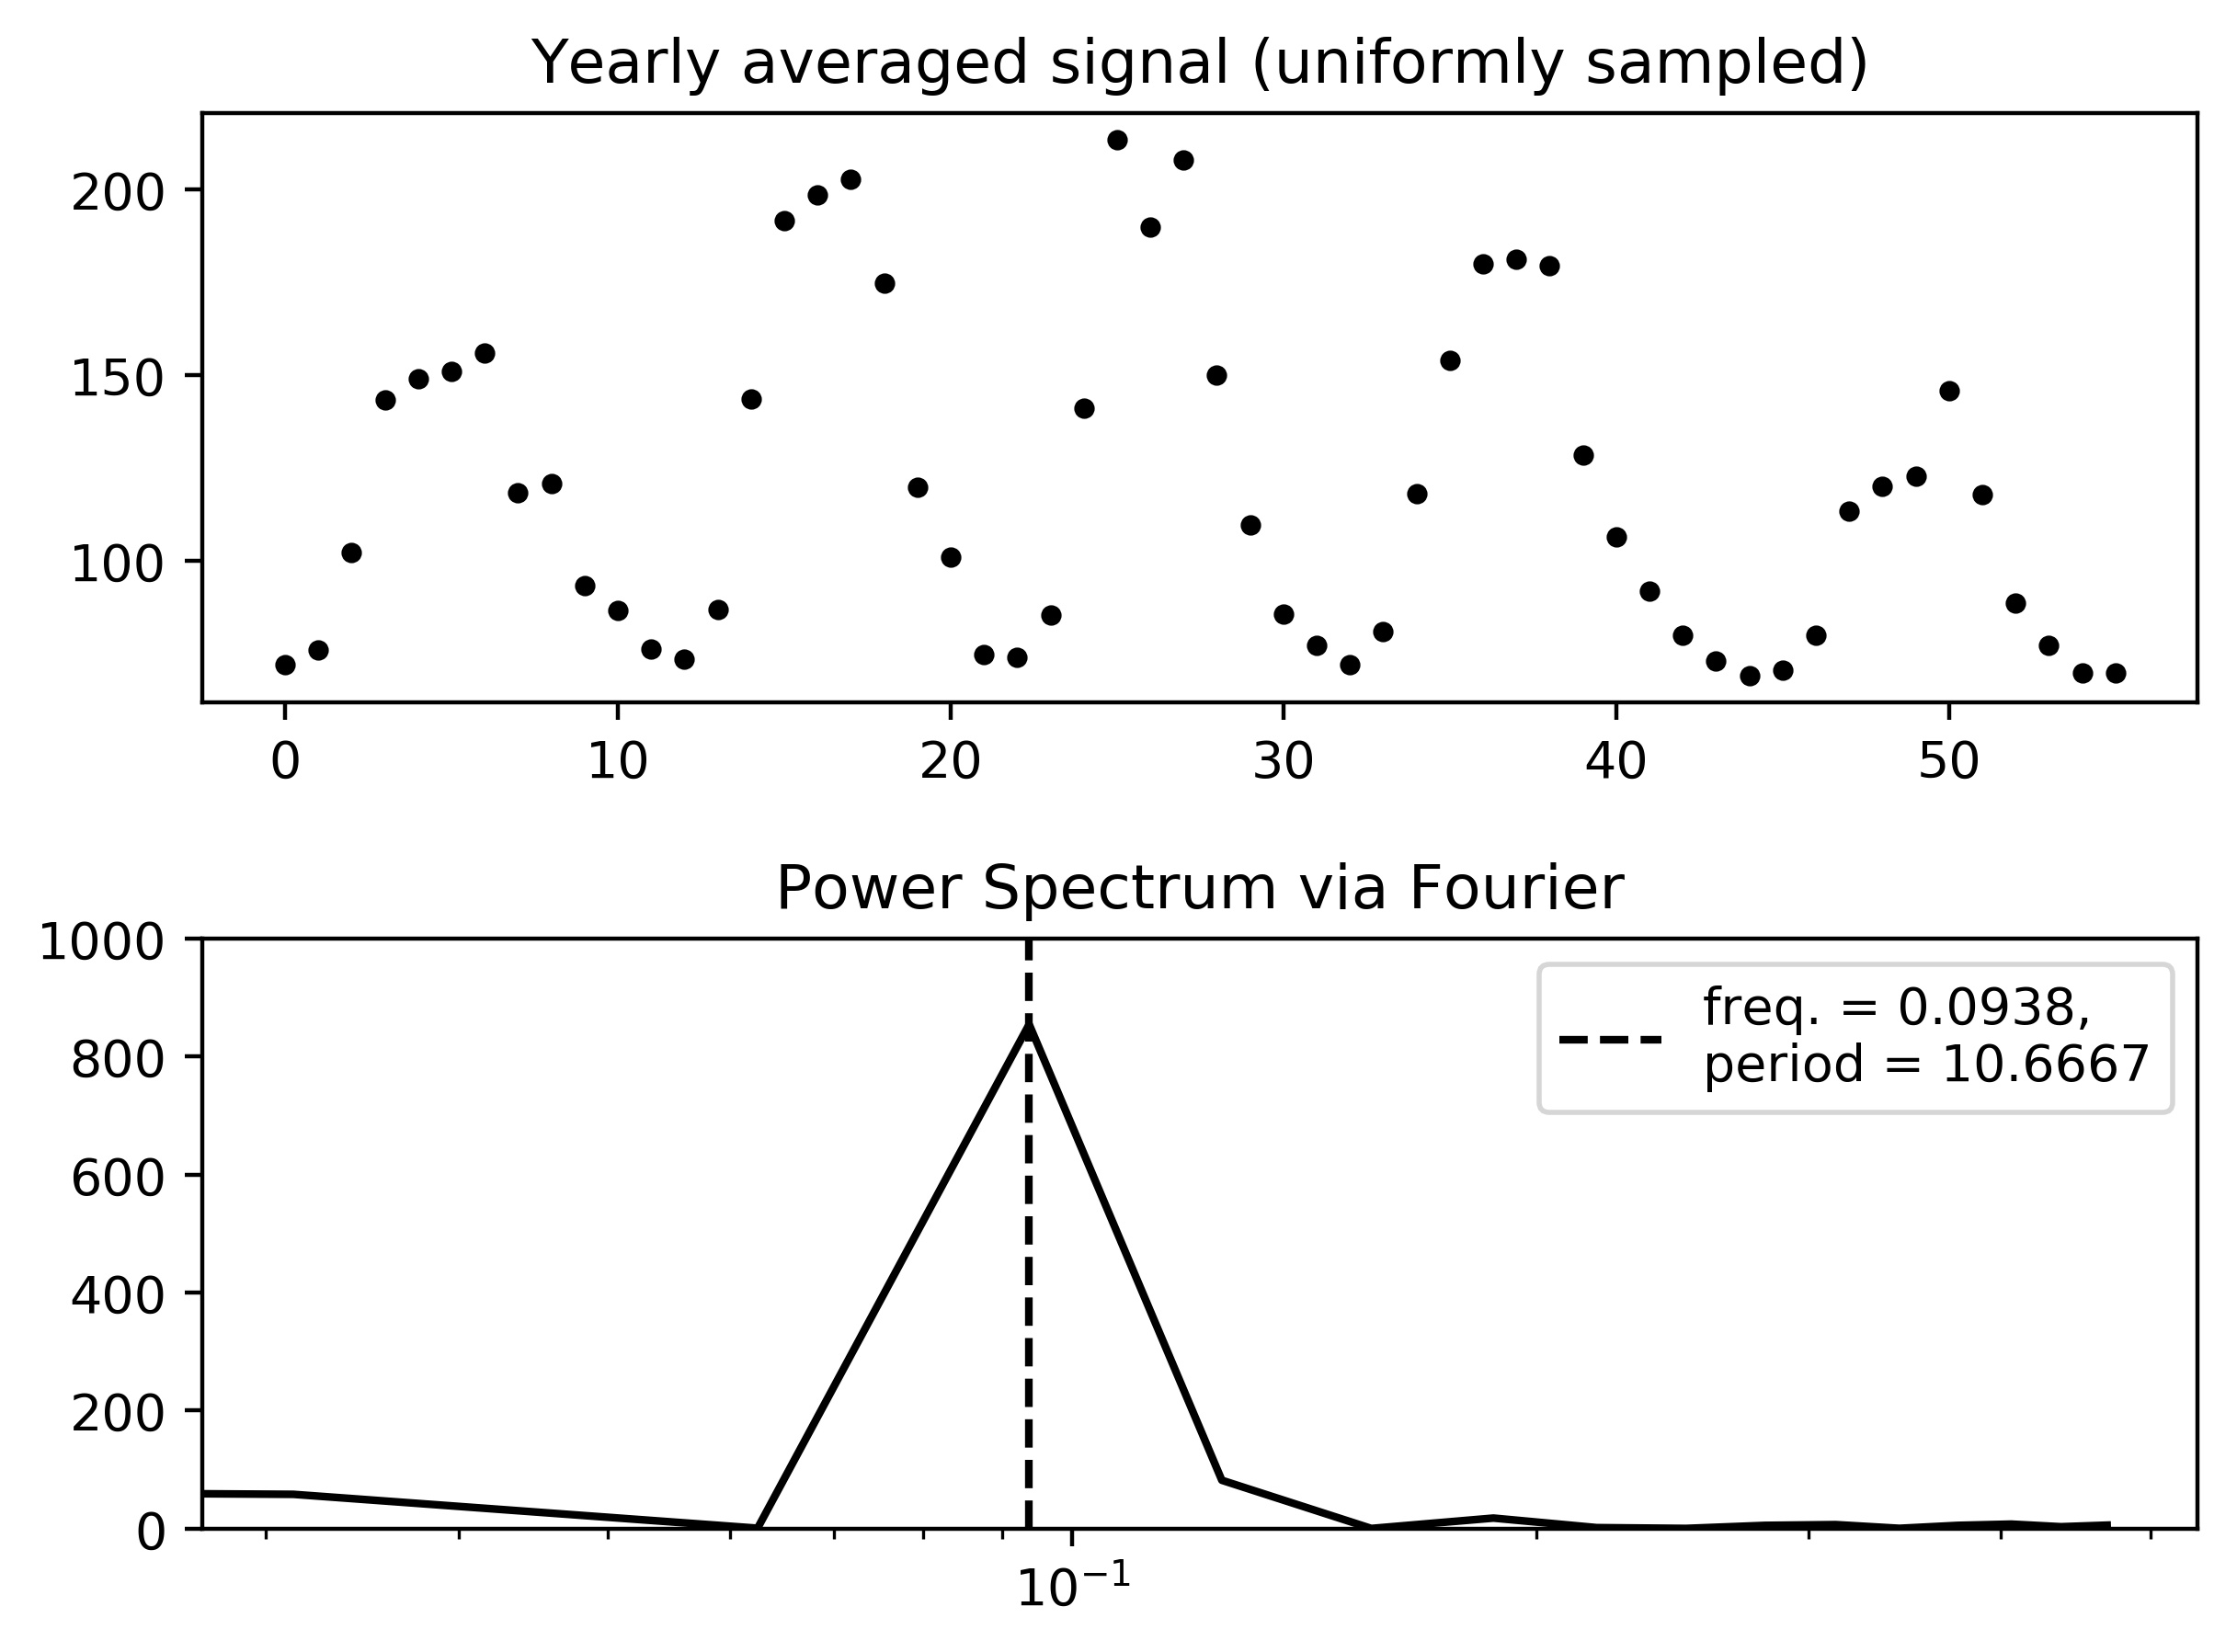
\includegraphics[scale=0.55]{Figuras/original_1.jpg}
\end{center}
\end{frame}

%%%%%%%%%%%%%%%%%%%%%%%%  FRAME  %%%%%%%%%%%%%%%%%%%%%%%%
\begin{frame}
\frametitle{Scenario 1 - yearly averages}
\begin{center}
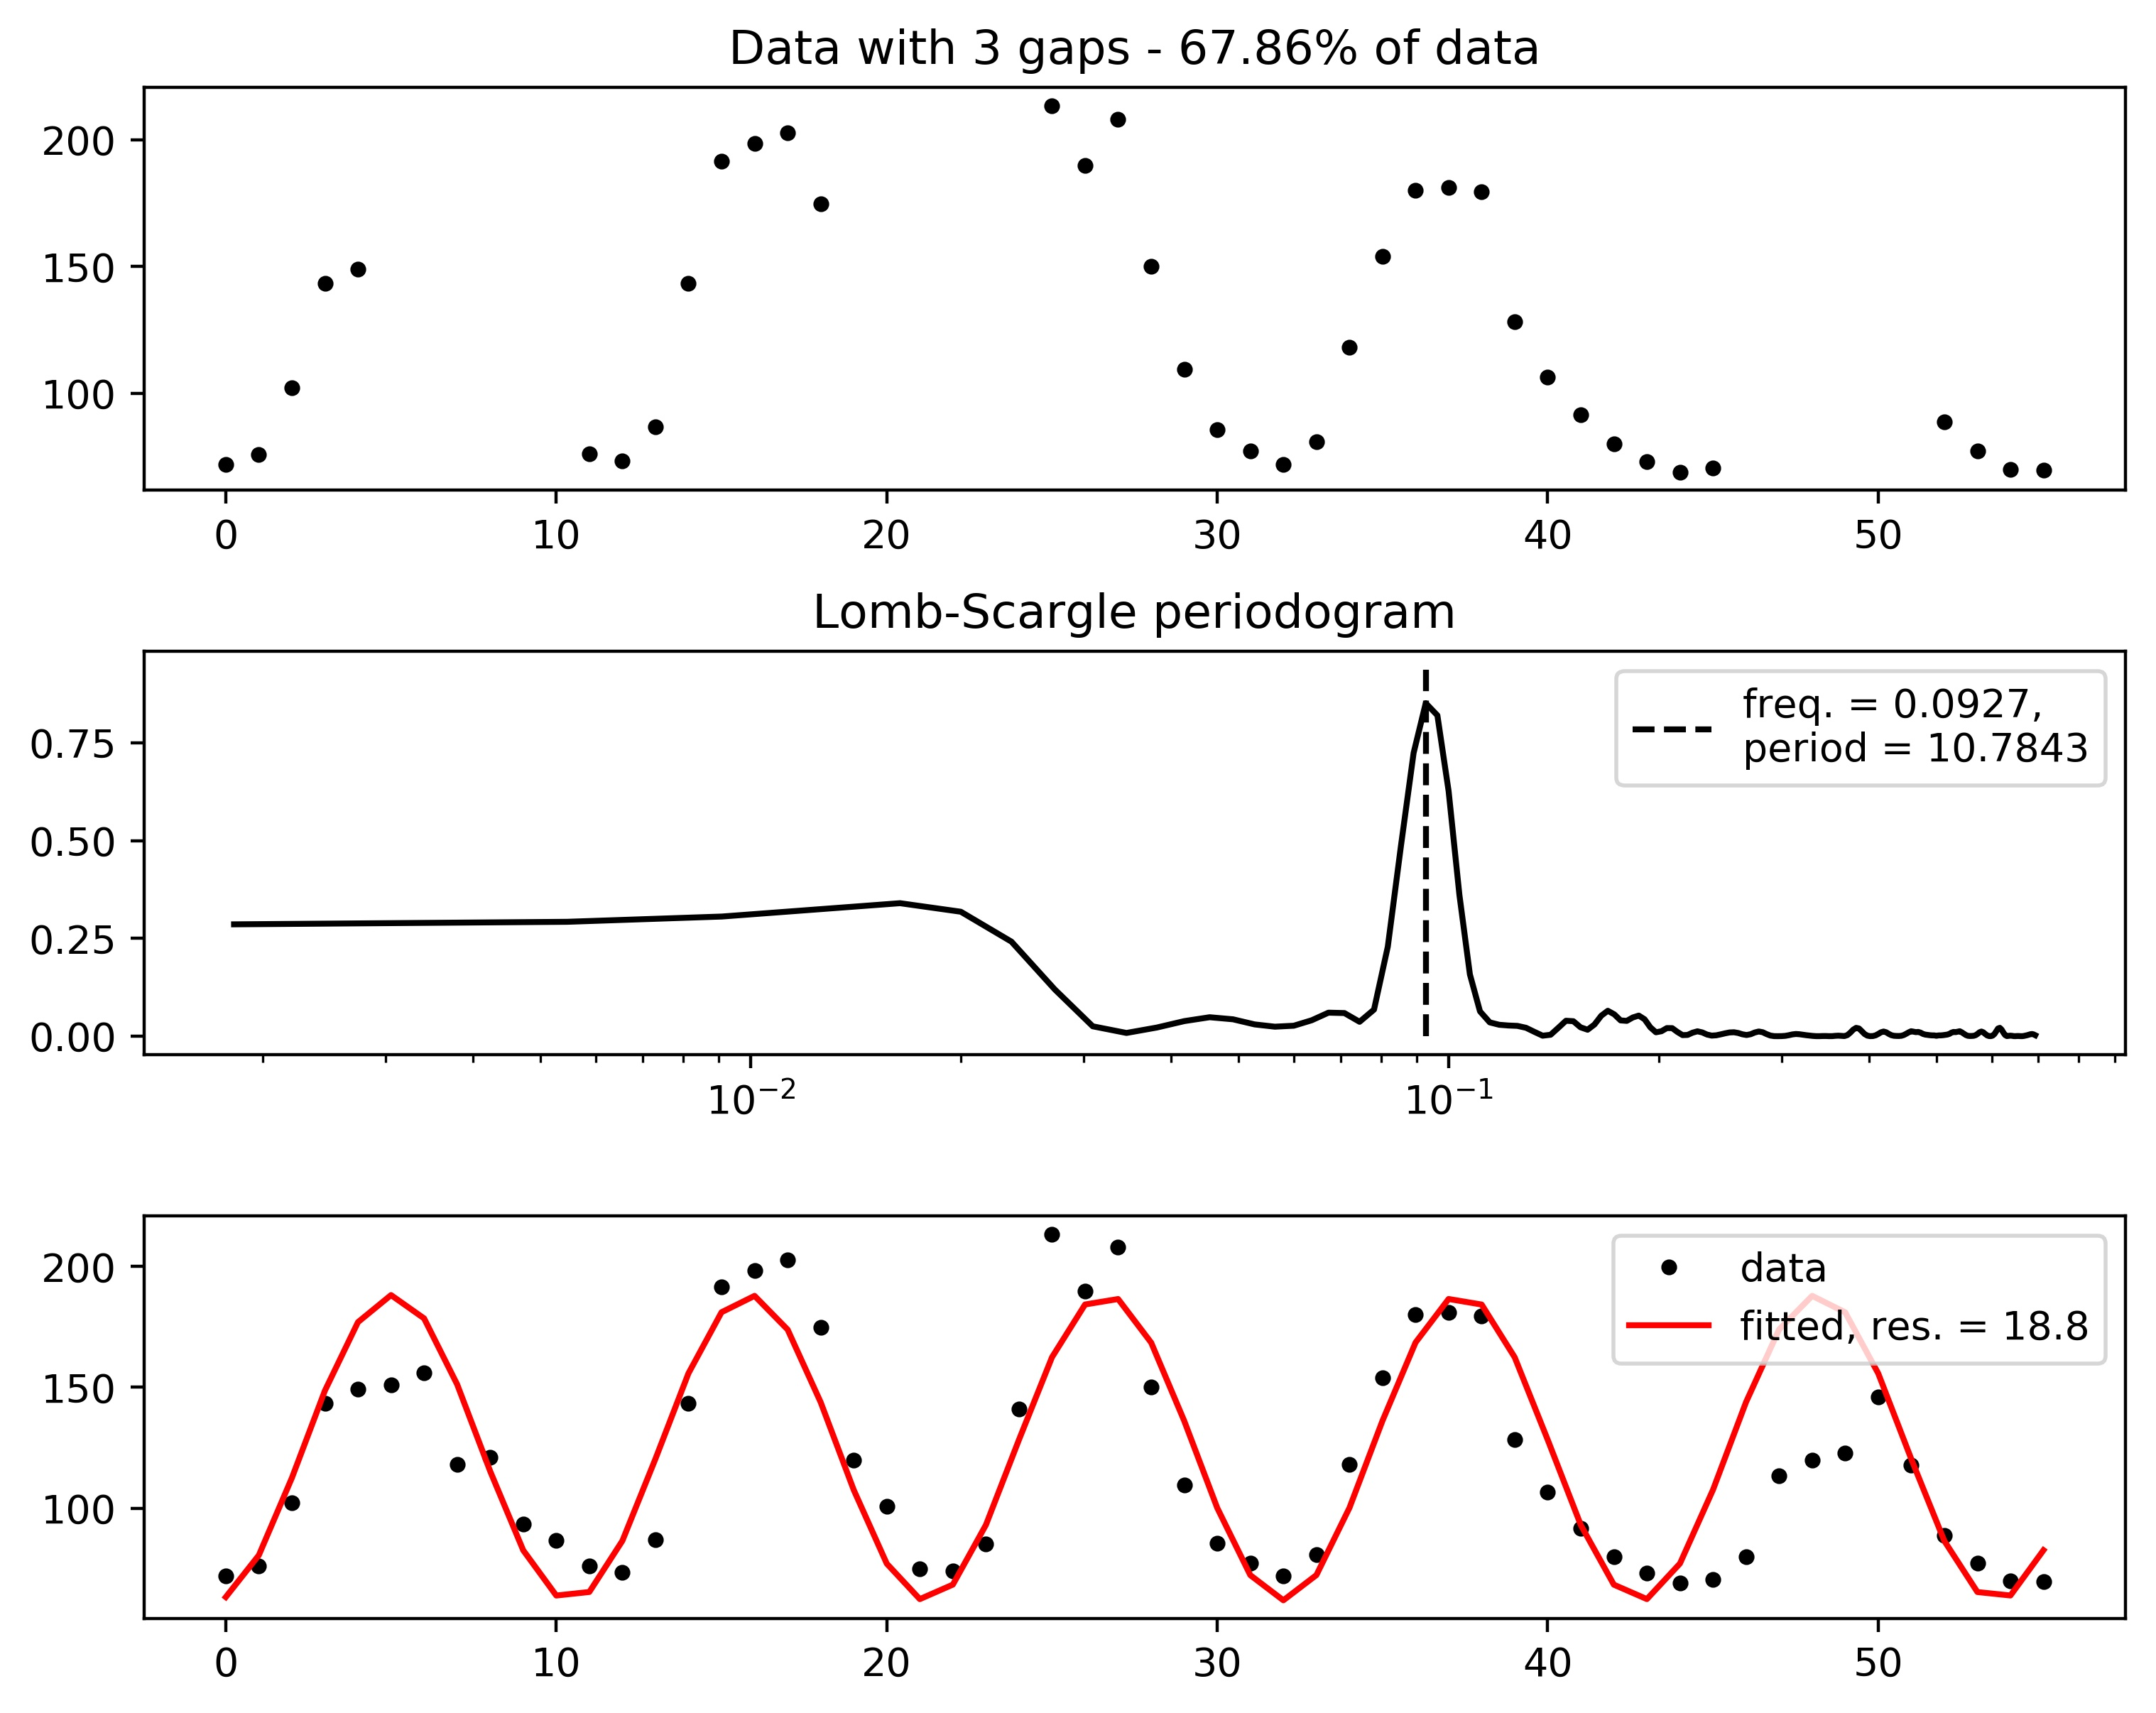
\includegraphics[scale=0.55]{../scripts/dataset3/periodograms_ny2.0_model2_Ng3.jpg}
\end{center}
\end{frame}
\begin{frame}
\frametitle{Scenario 1 - yearly averages}
\begin{center}
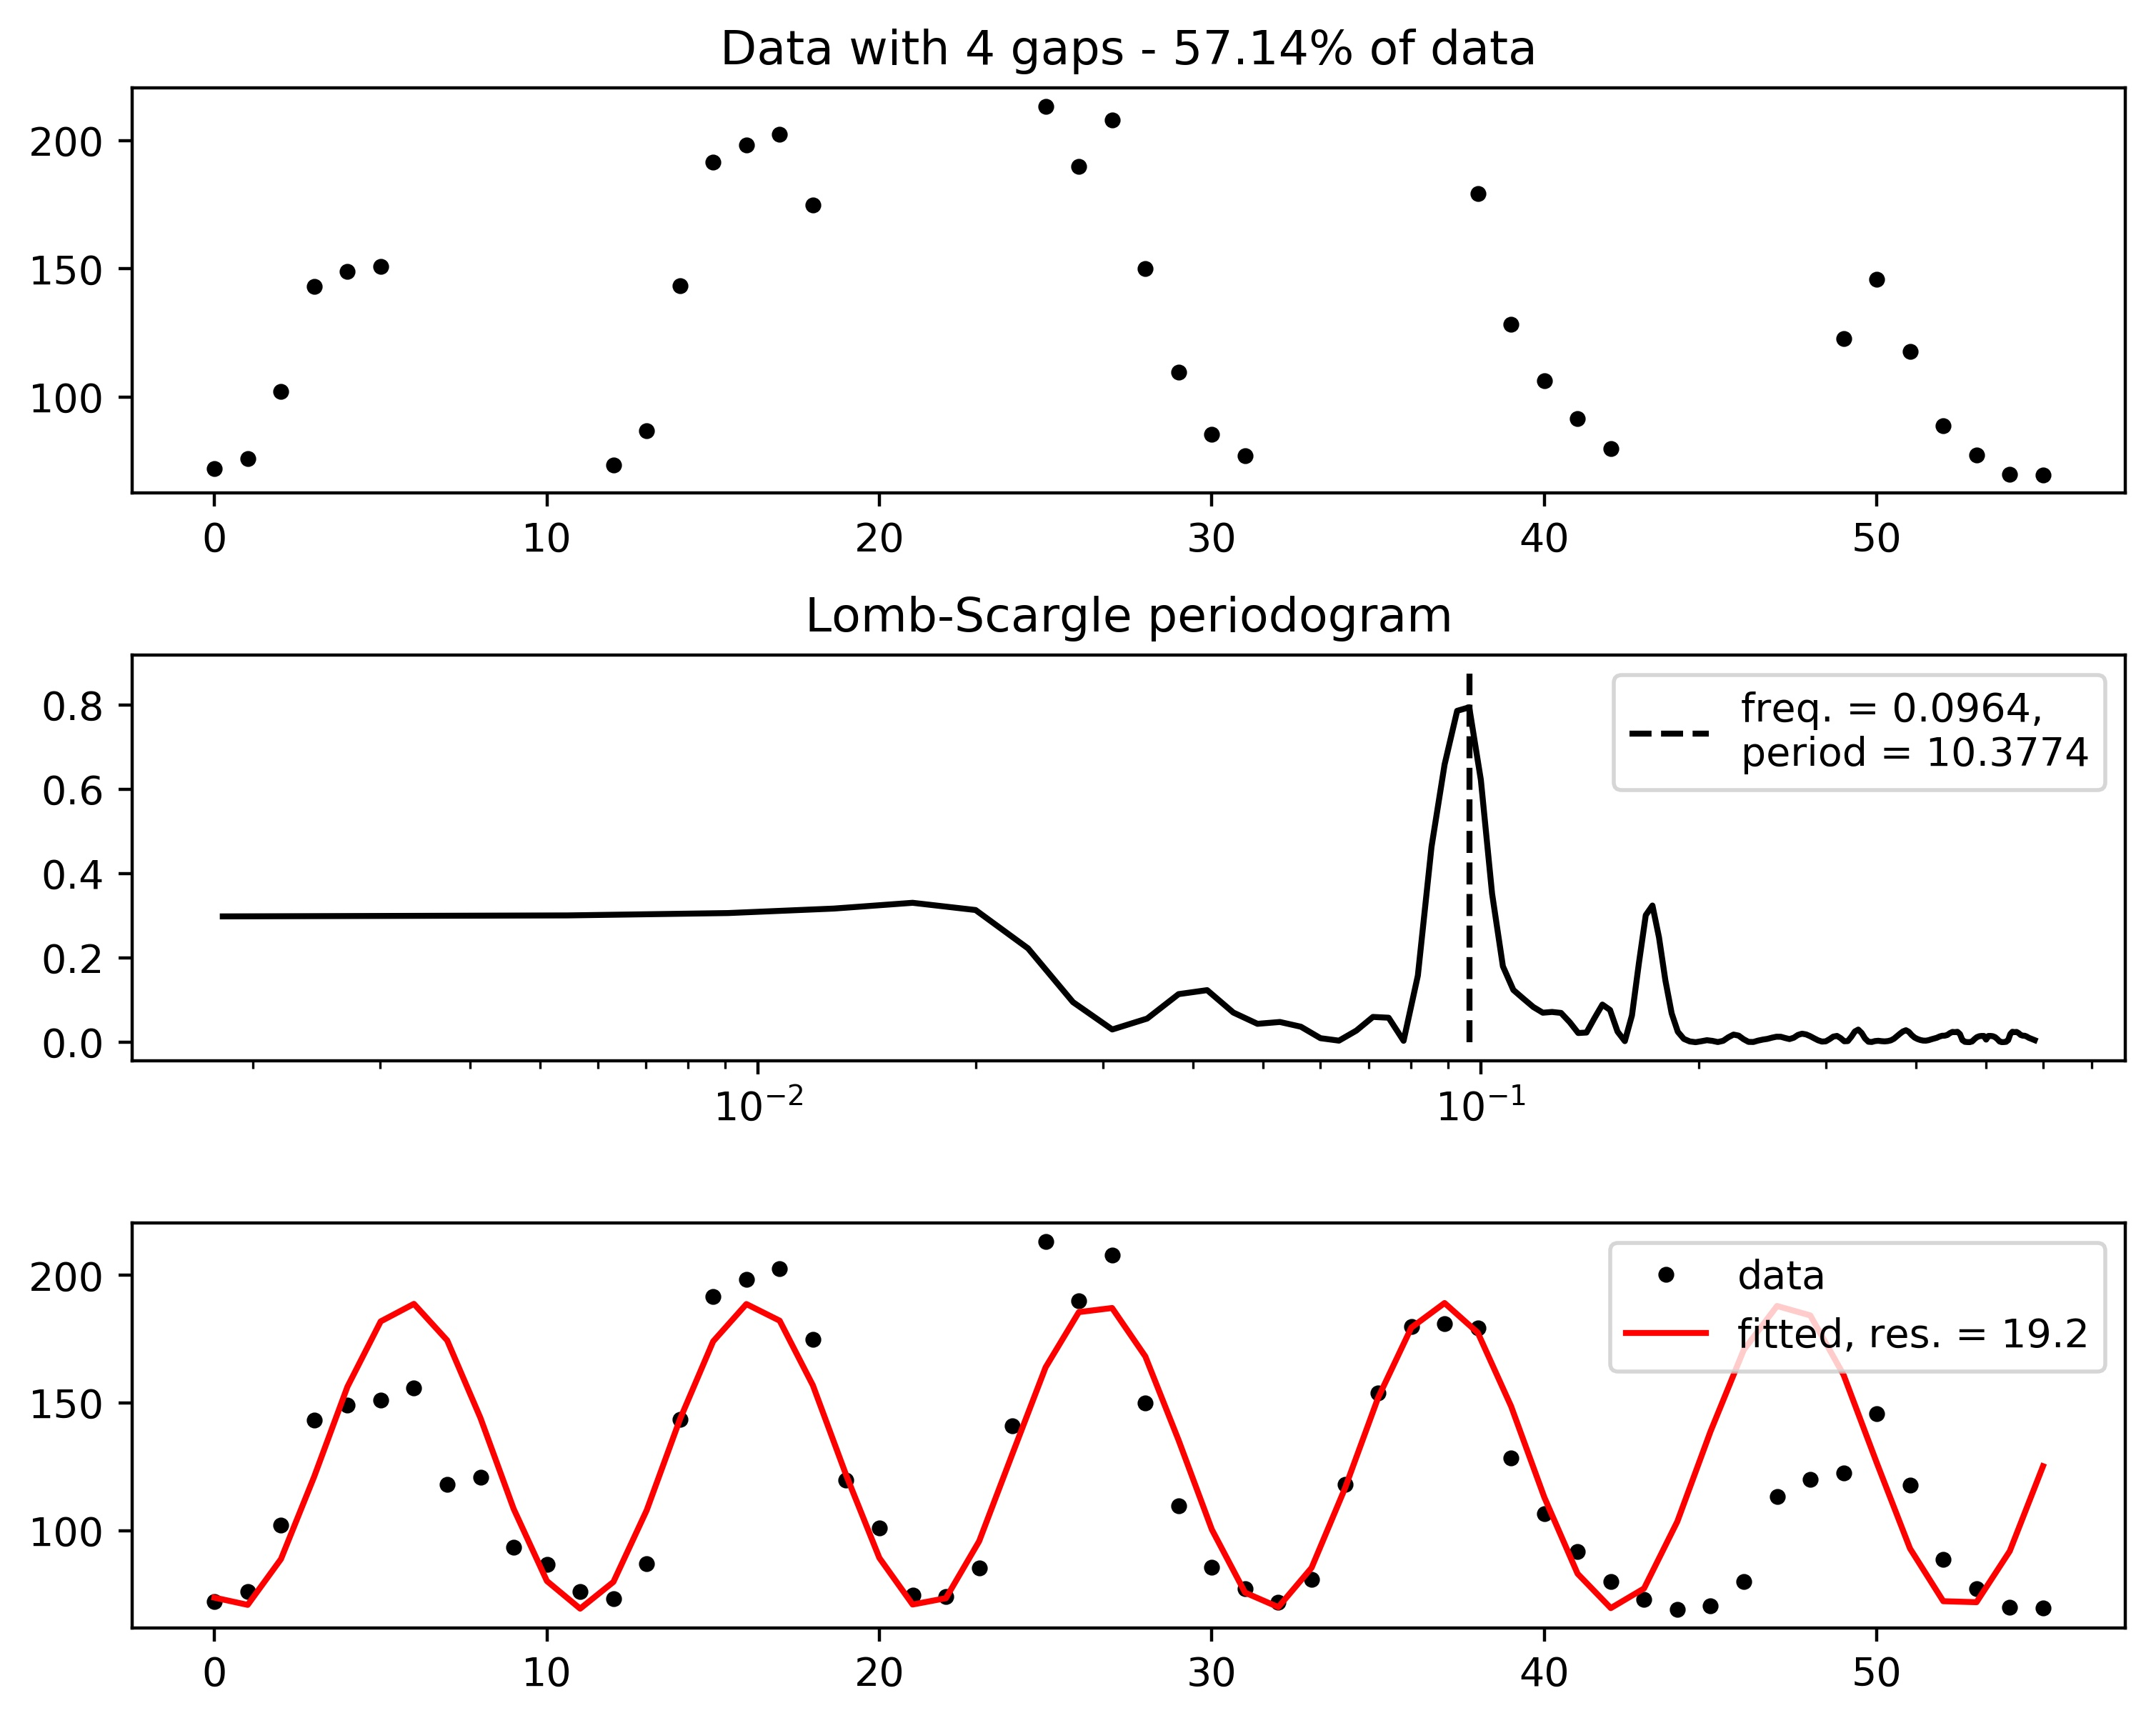
\includegraphics[scale=0.55]{../scripts/dataset3/periodograms_ny2.0_model2_Ng4.jpg}
\end{center}
\end{frame}
\begin{frame}
\frametitle{Scenario 1 - yearly averages}
\begin{center}
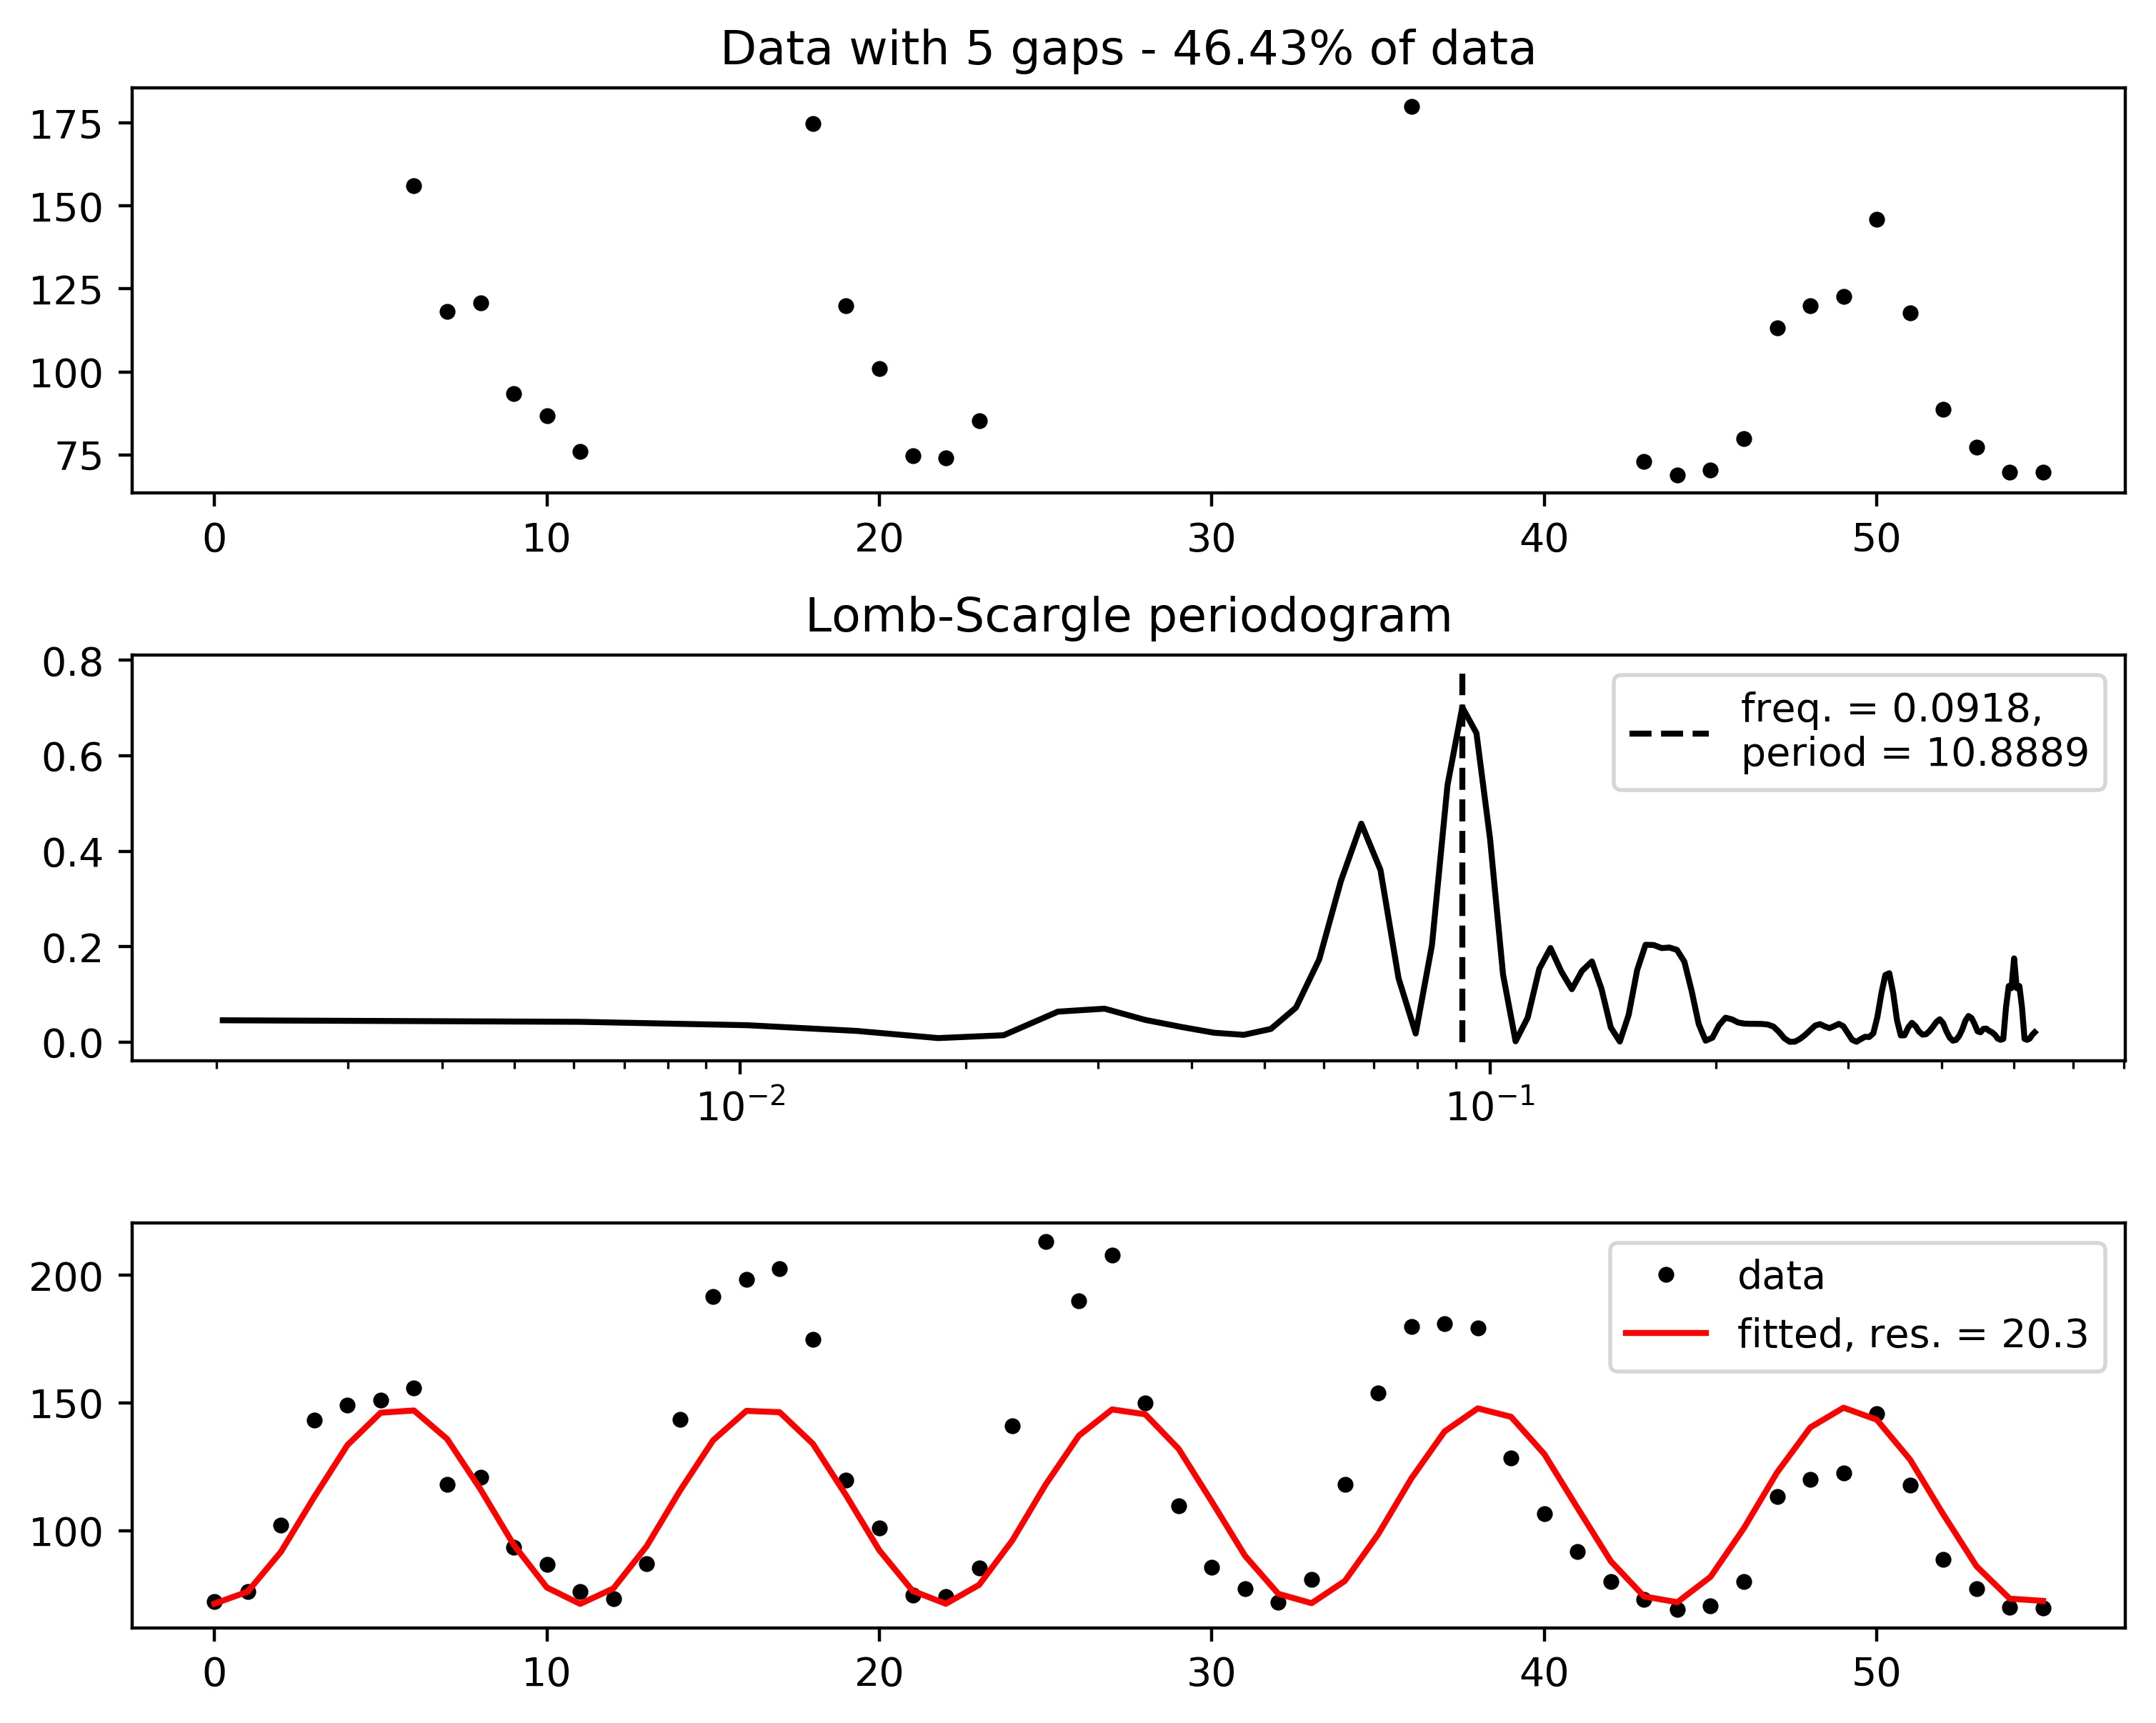
\includegraphics[scale=0.55]{../scripts/dataset3/periodograms_ny2.0_model2_Ng5.jpg}
\end{center}
\end{frame}
\begin{frame}
\frametitle{Scenario 1 - yearly averages}
\begin{center}
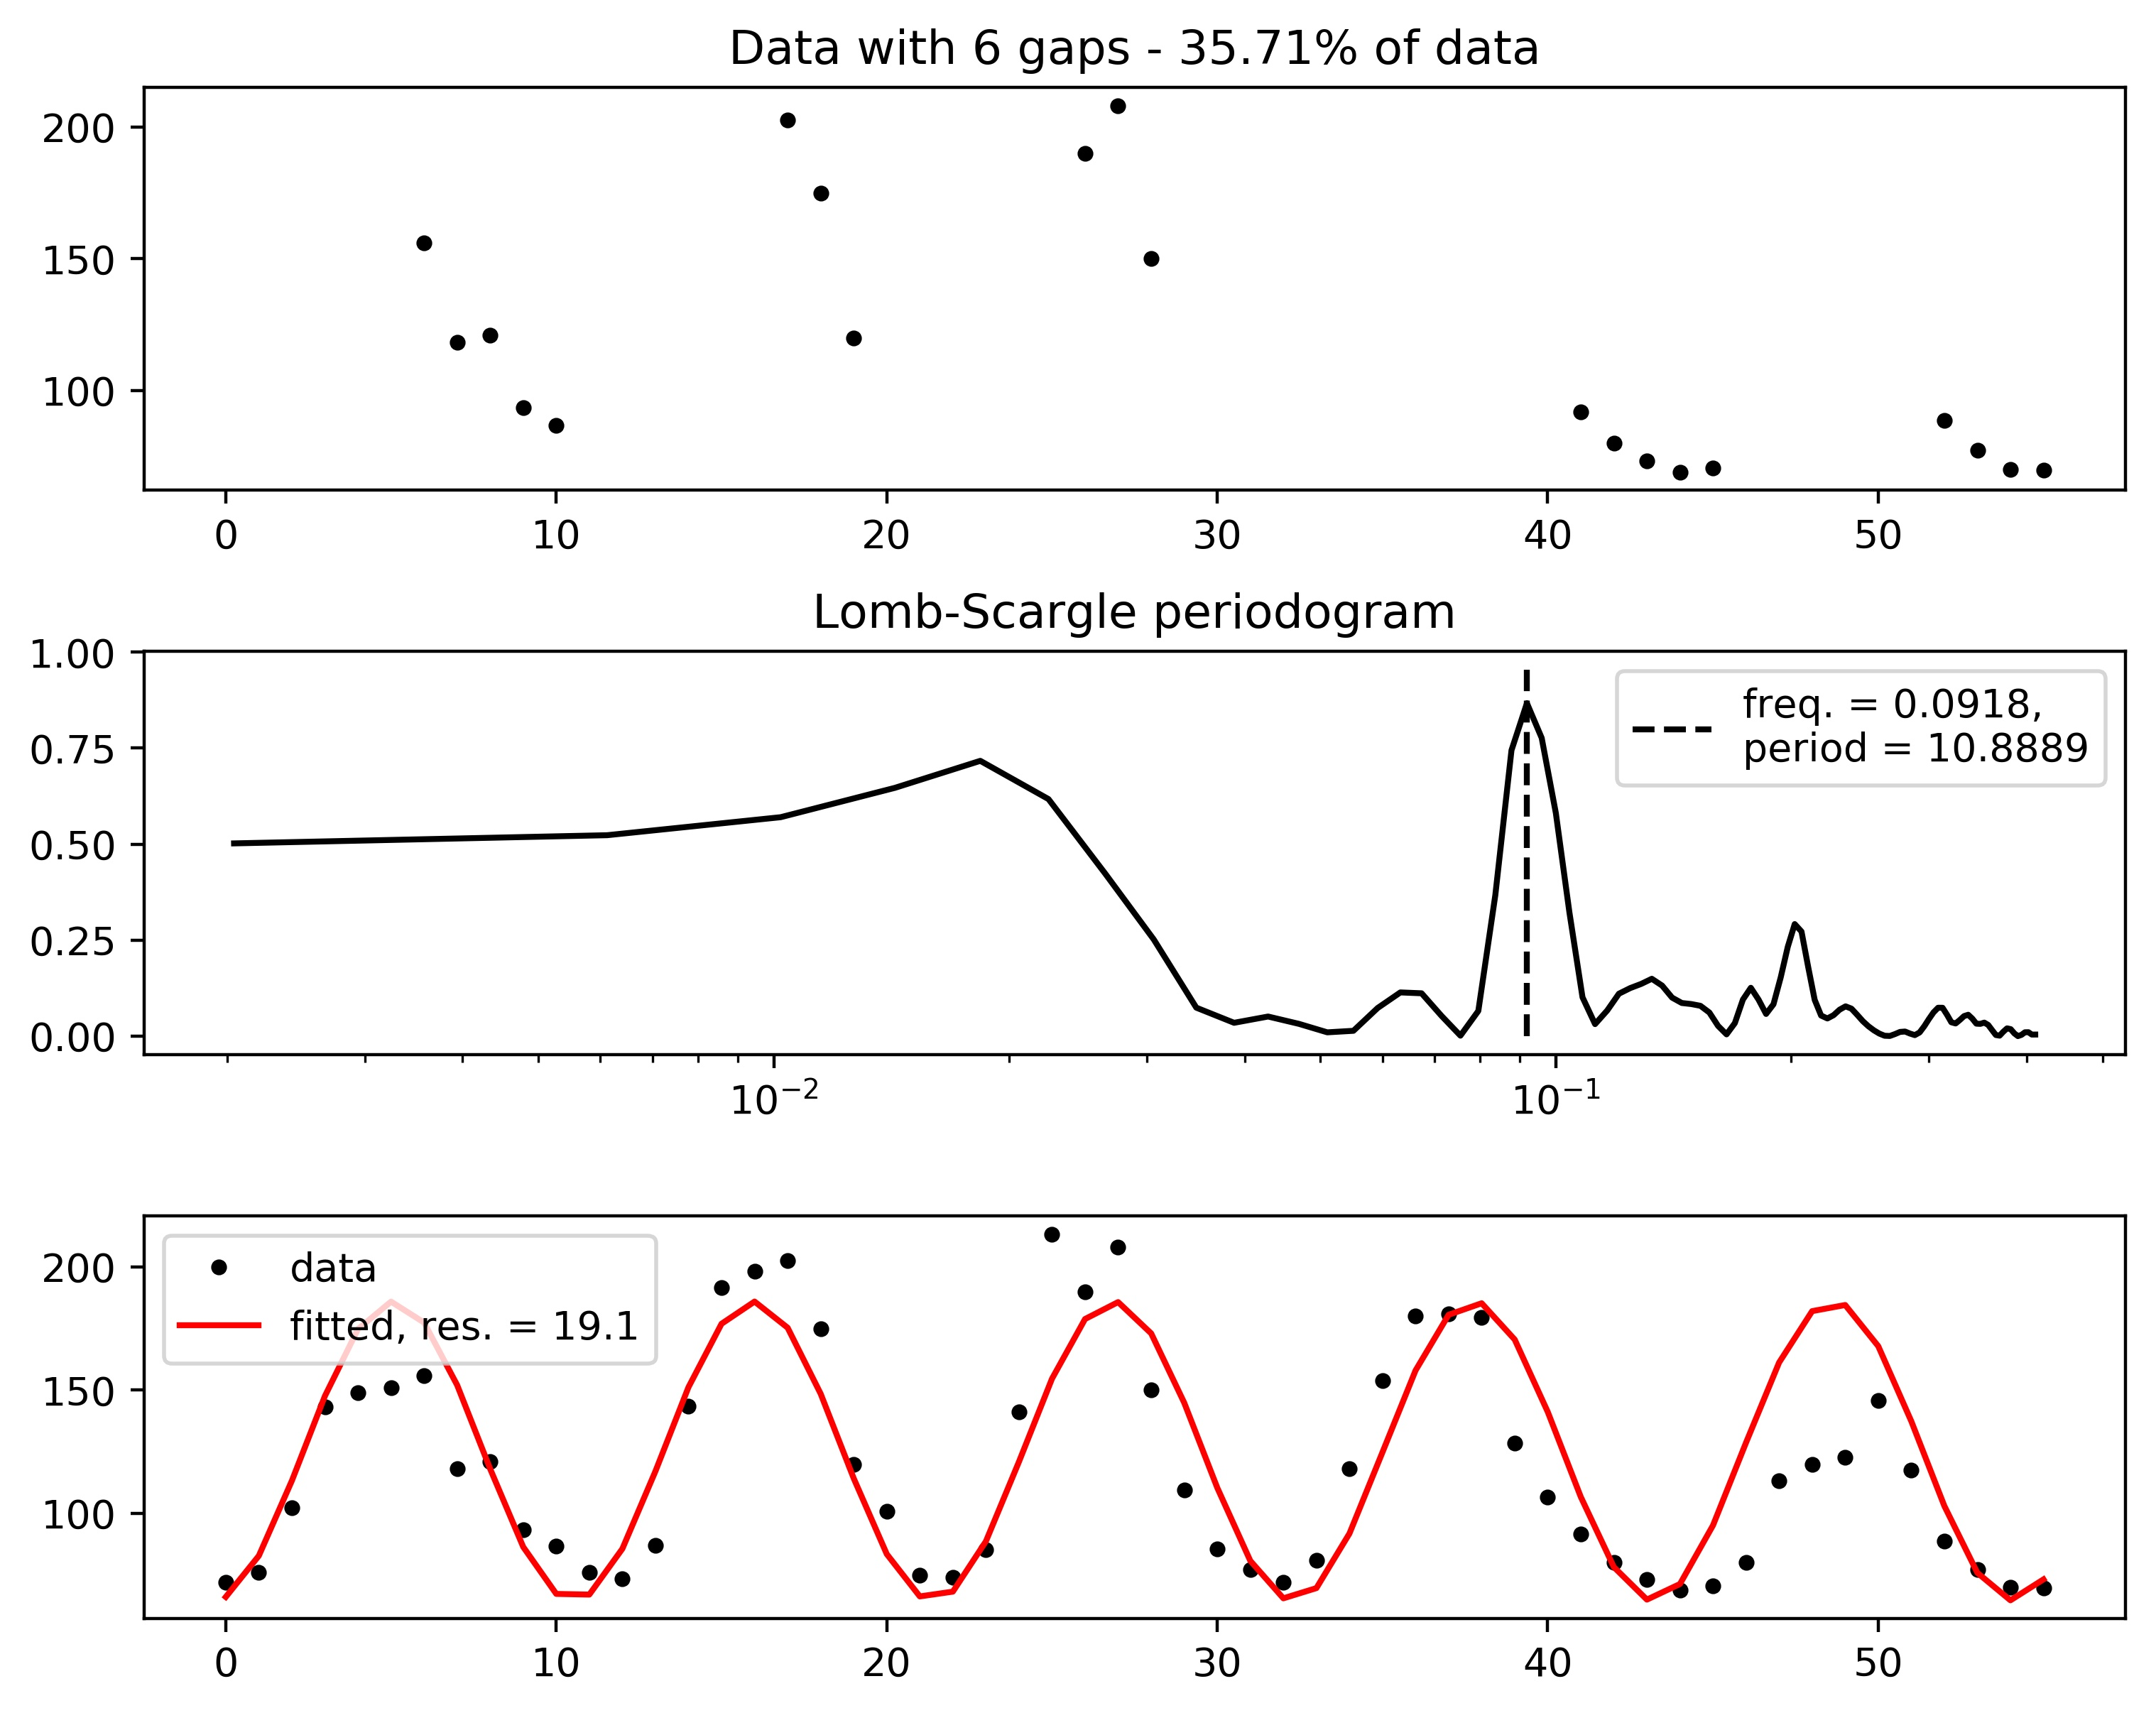
\includegraphics[scale=0.55]{../scripts/dataset3/periodograms_ny2.0_model2_Ng6.jpg}
\end{center}
\end{frame}
\begin{frame}
\frametitle{Scenario 1 - yearly averages}
\begin{center}
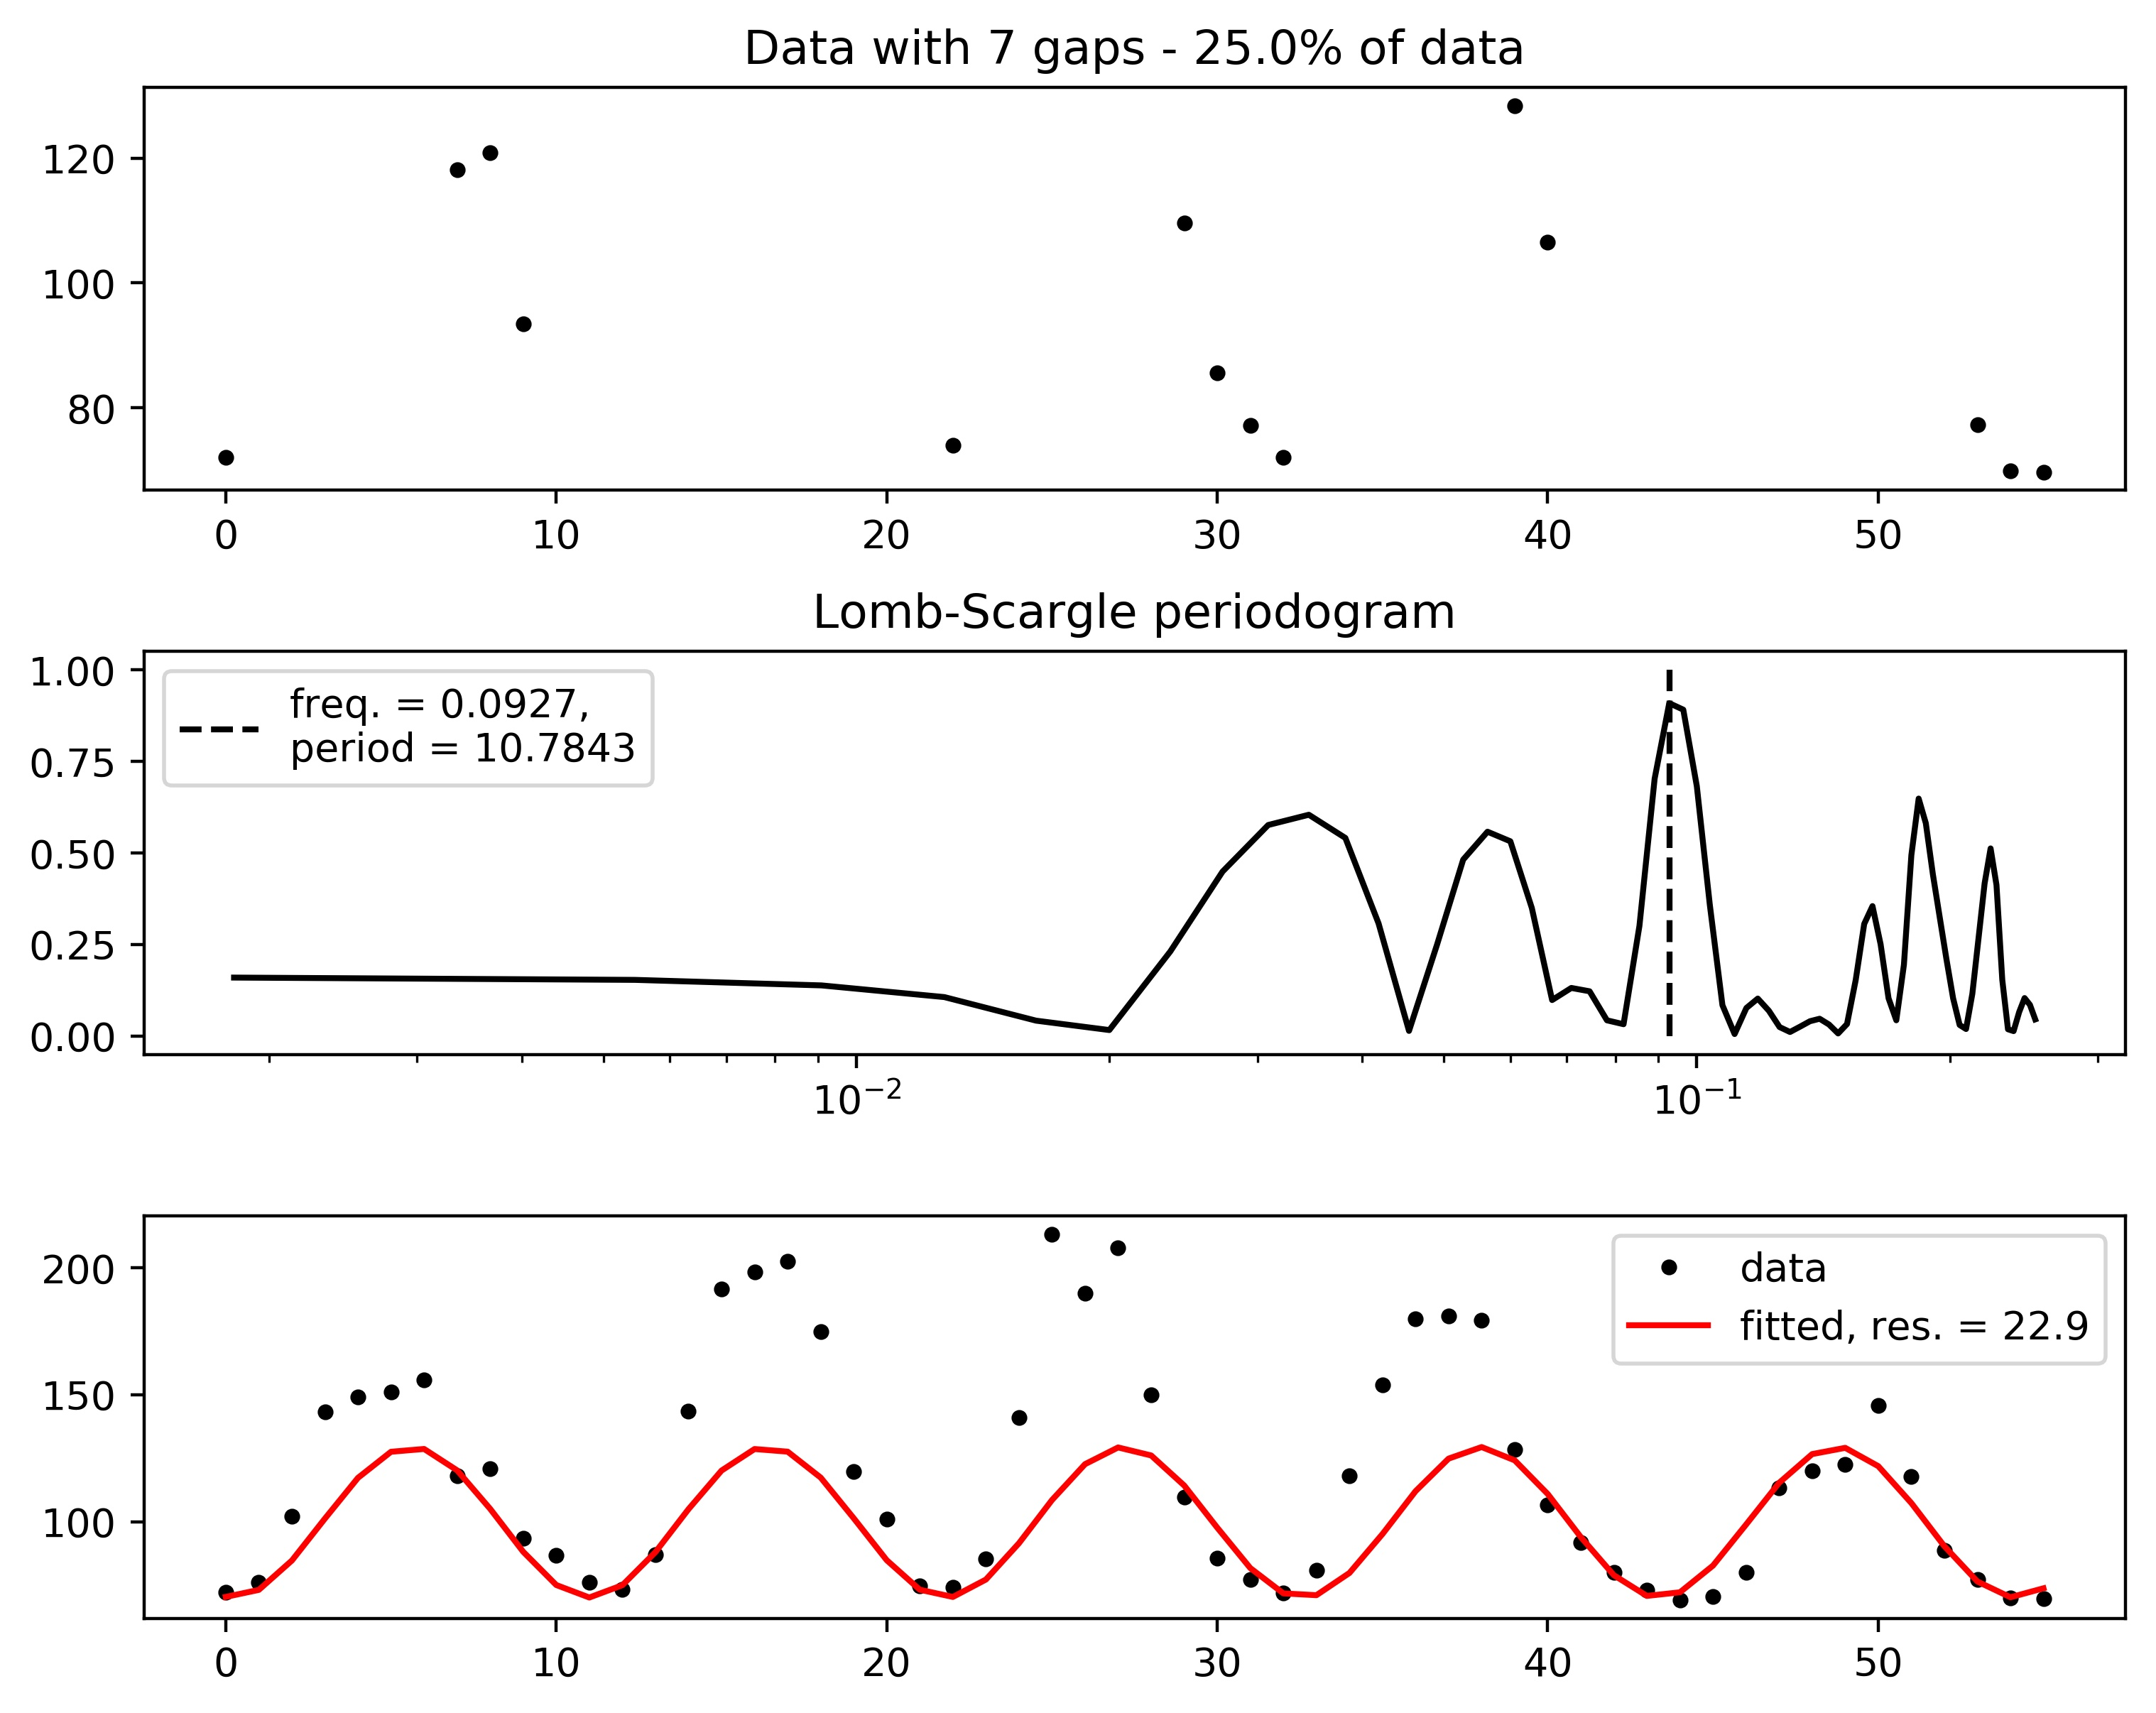
\includegraphics[scale=0.55]{../scripts/dataset3/periodograms_ny2.0_model2_Ng7.jpg}
\end{center}
\end{frame}

%%%%%%%%%%%%%%%%%%%%%%%%  FRAME  %%%%%%%%%%%%%%%%%%%%%%%%
\begin{frame}
\frametitle{Scenario 2 - daily averages}
\begin{center}
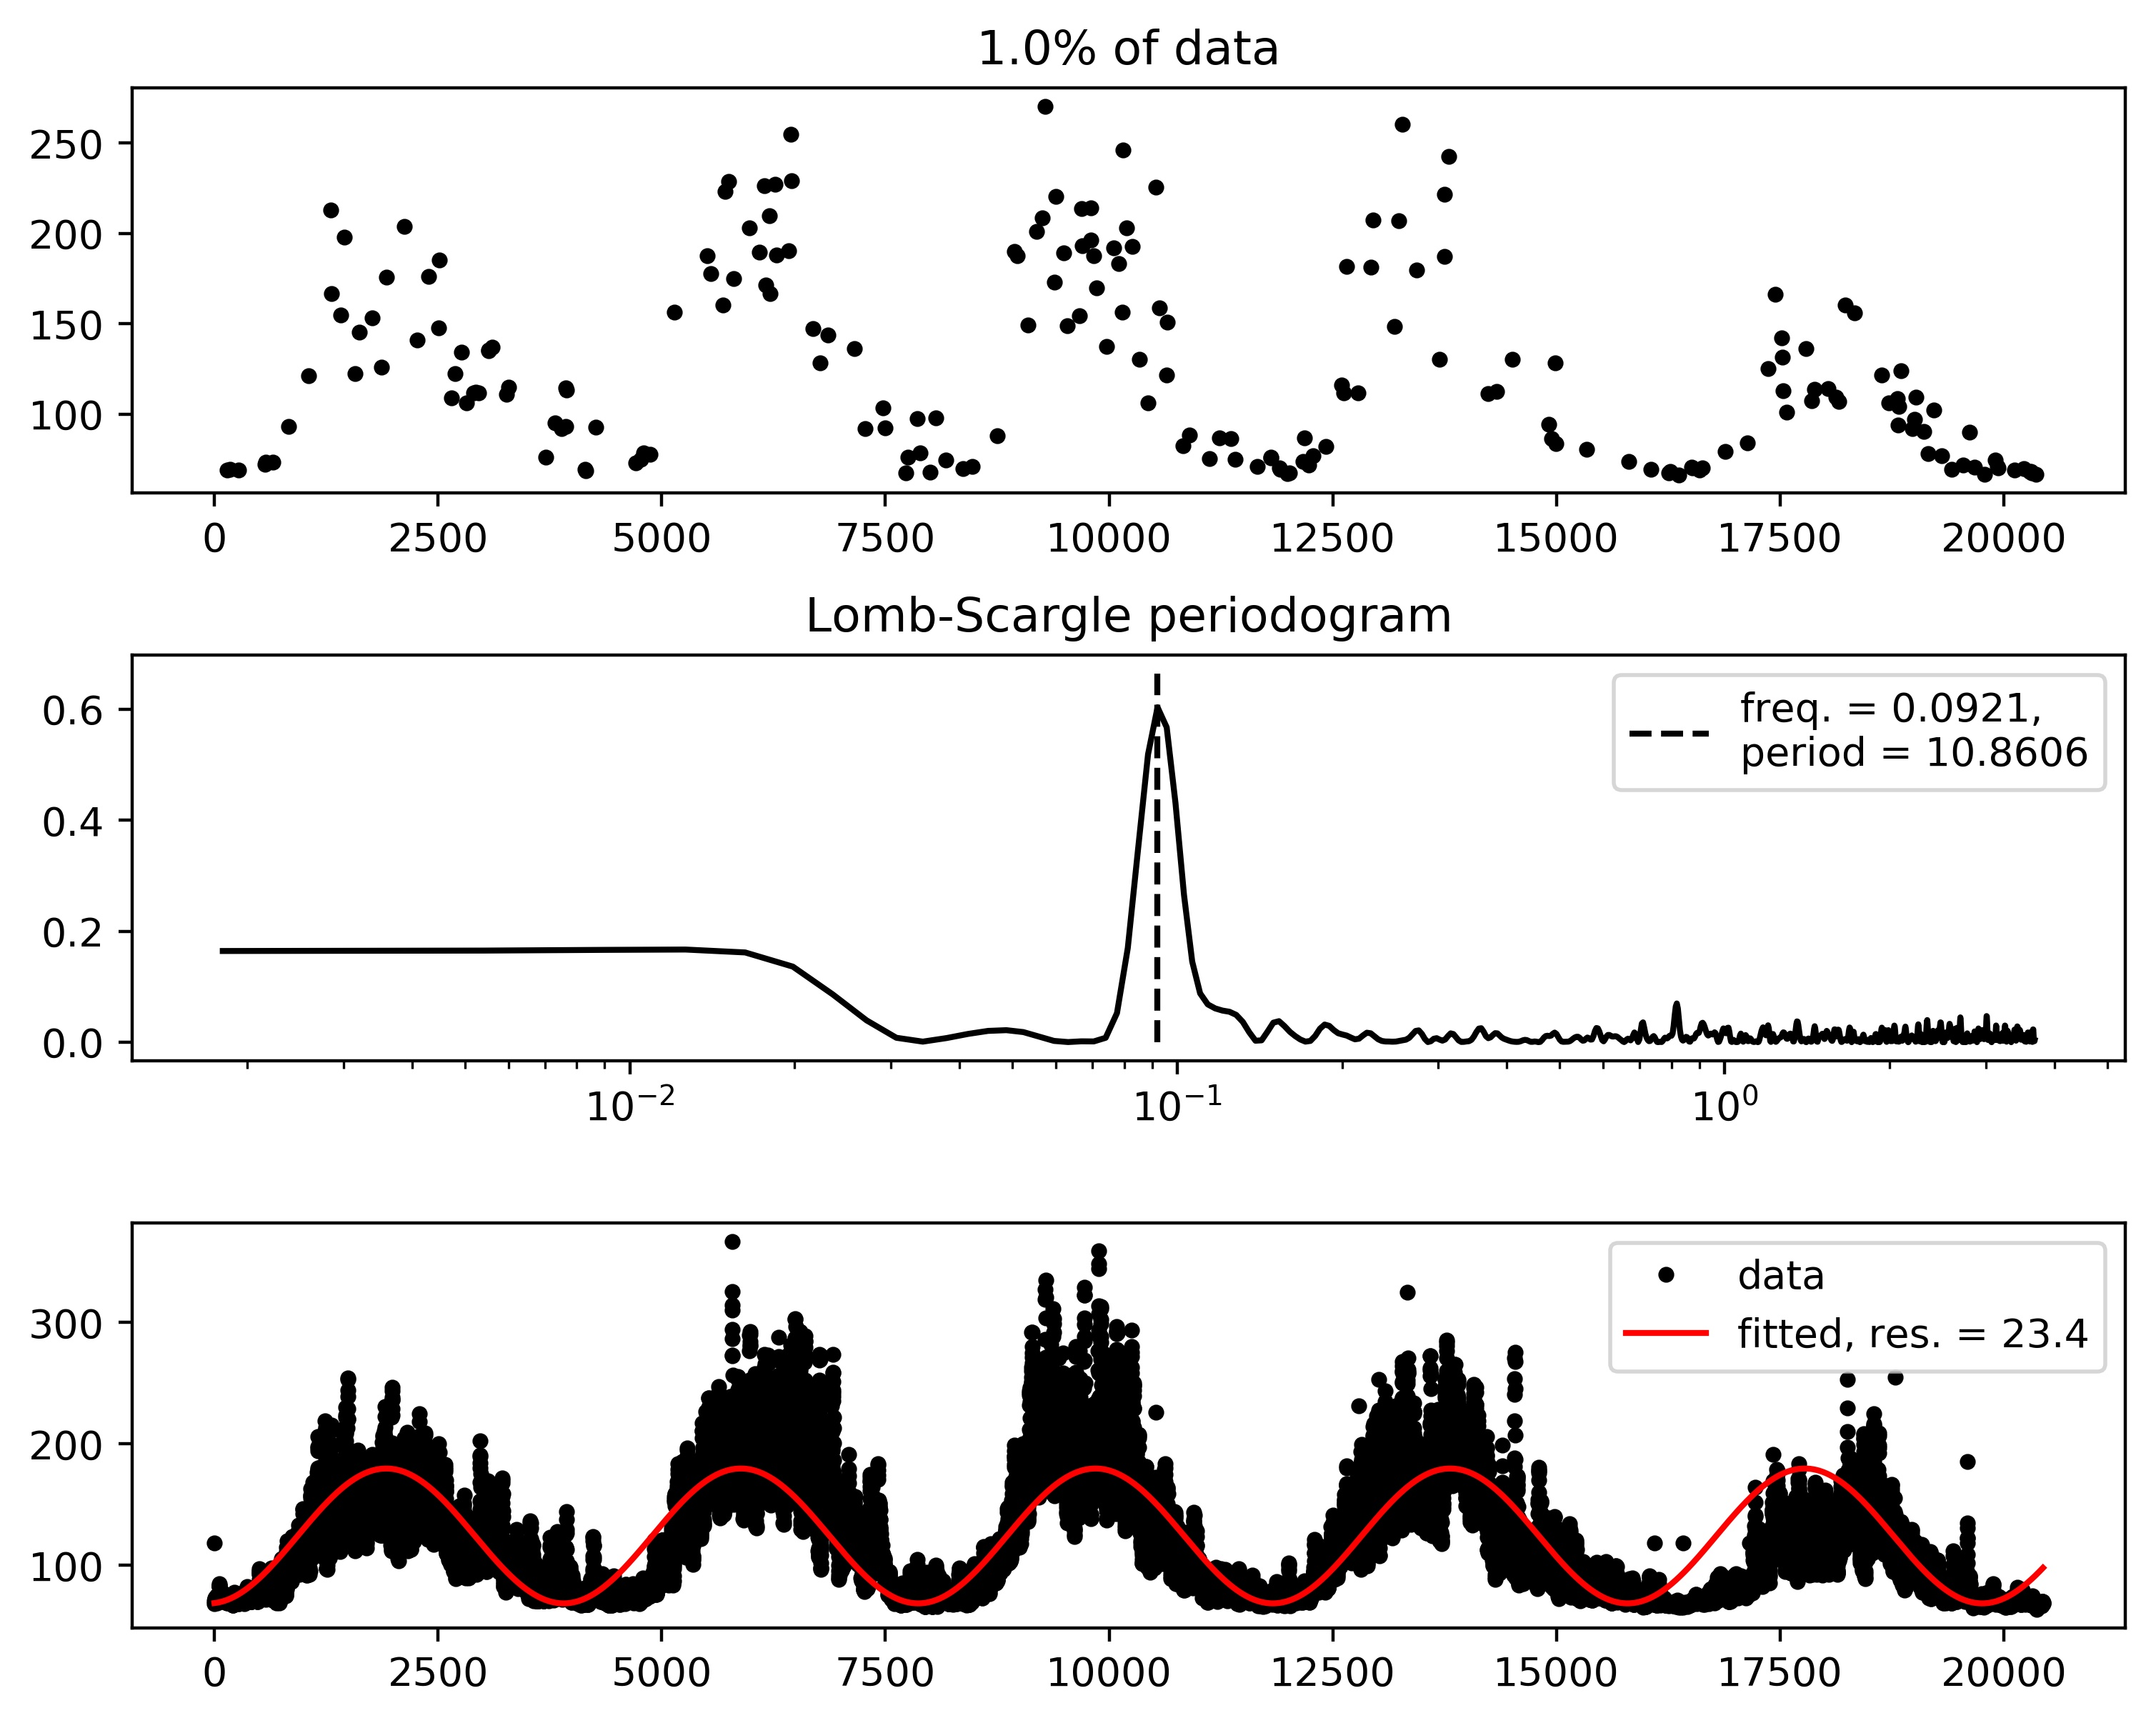
\includegraphics[scale=0.55]{../scripts/dataset1/periodograms_ny2.0_model1_pg0.99.jpg}
\end{center}
\end{frame}
\begin{frame}
\frametitle{Scenario 2 - daily averages}
\begin{center}
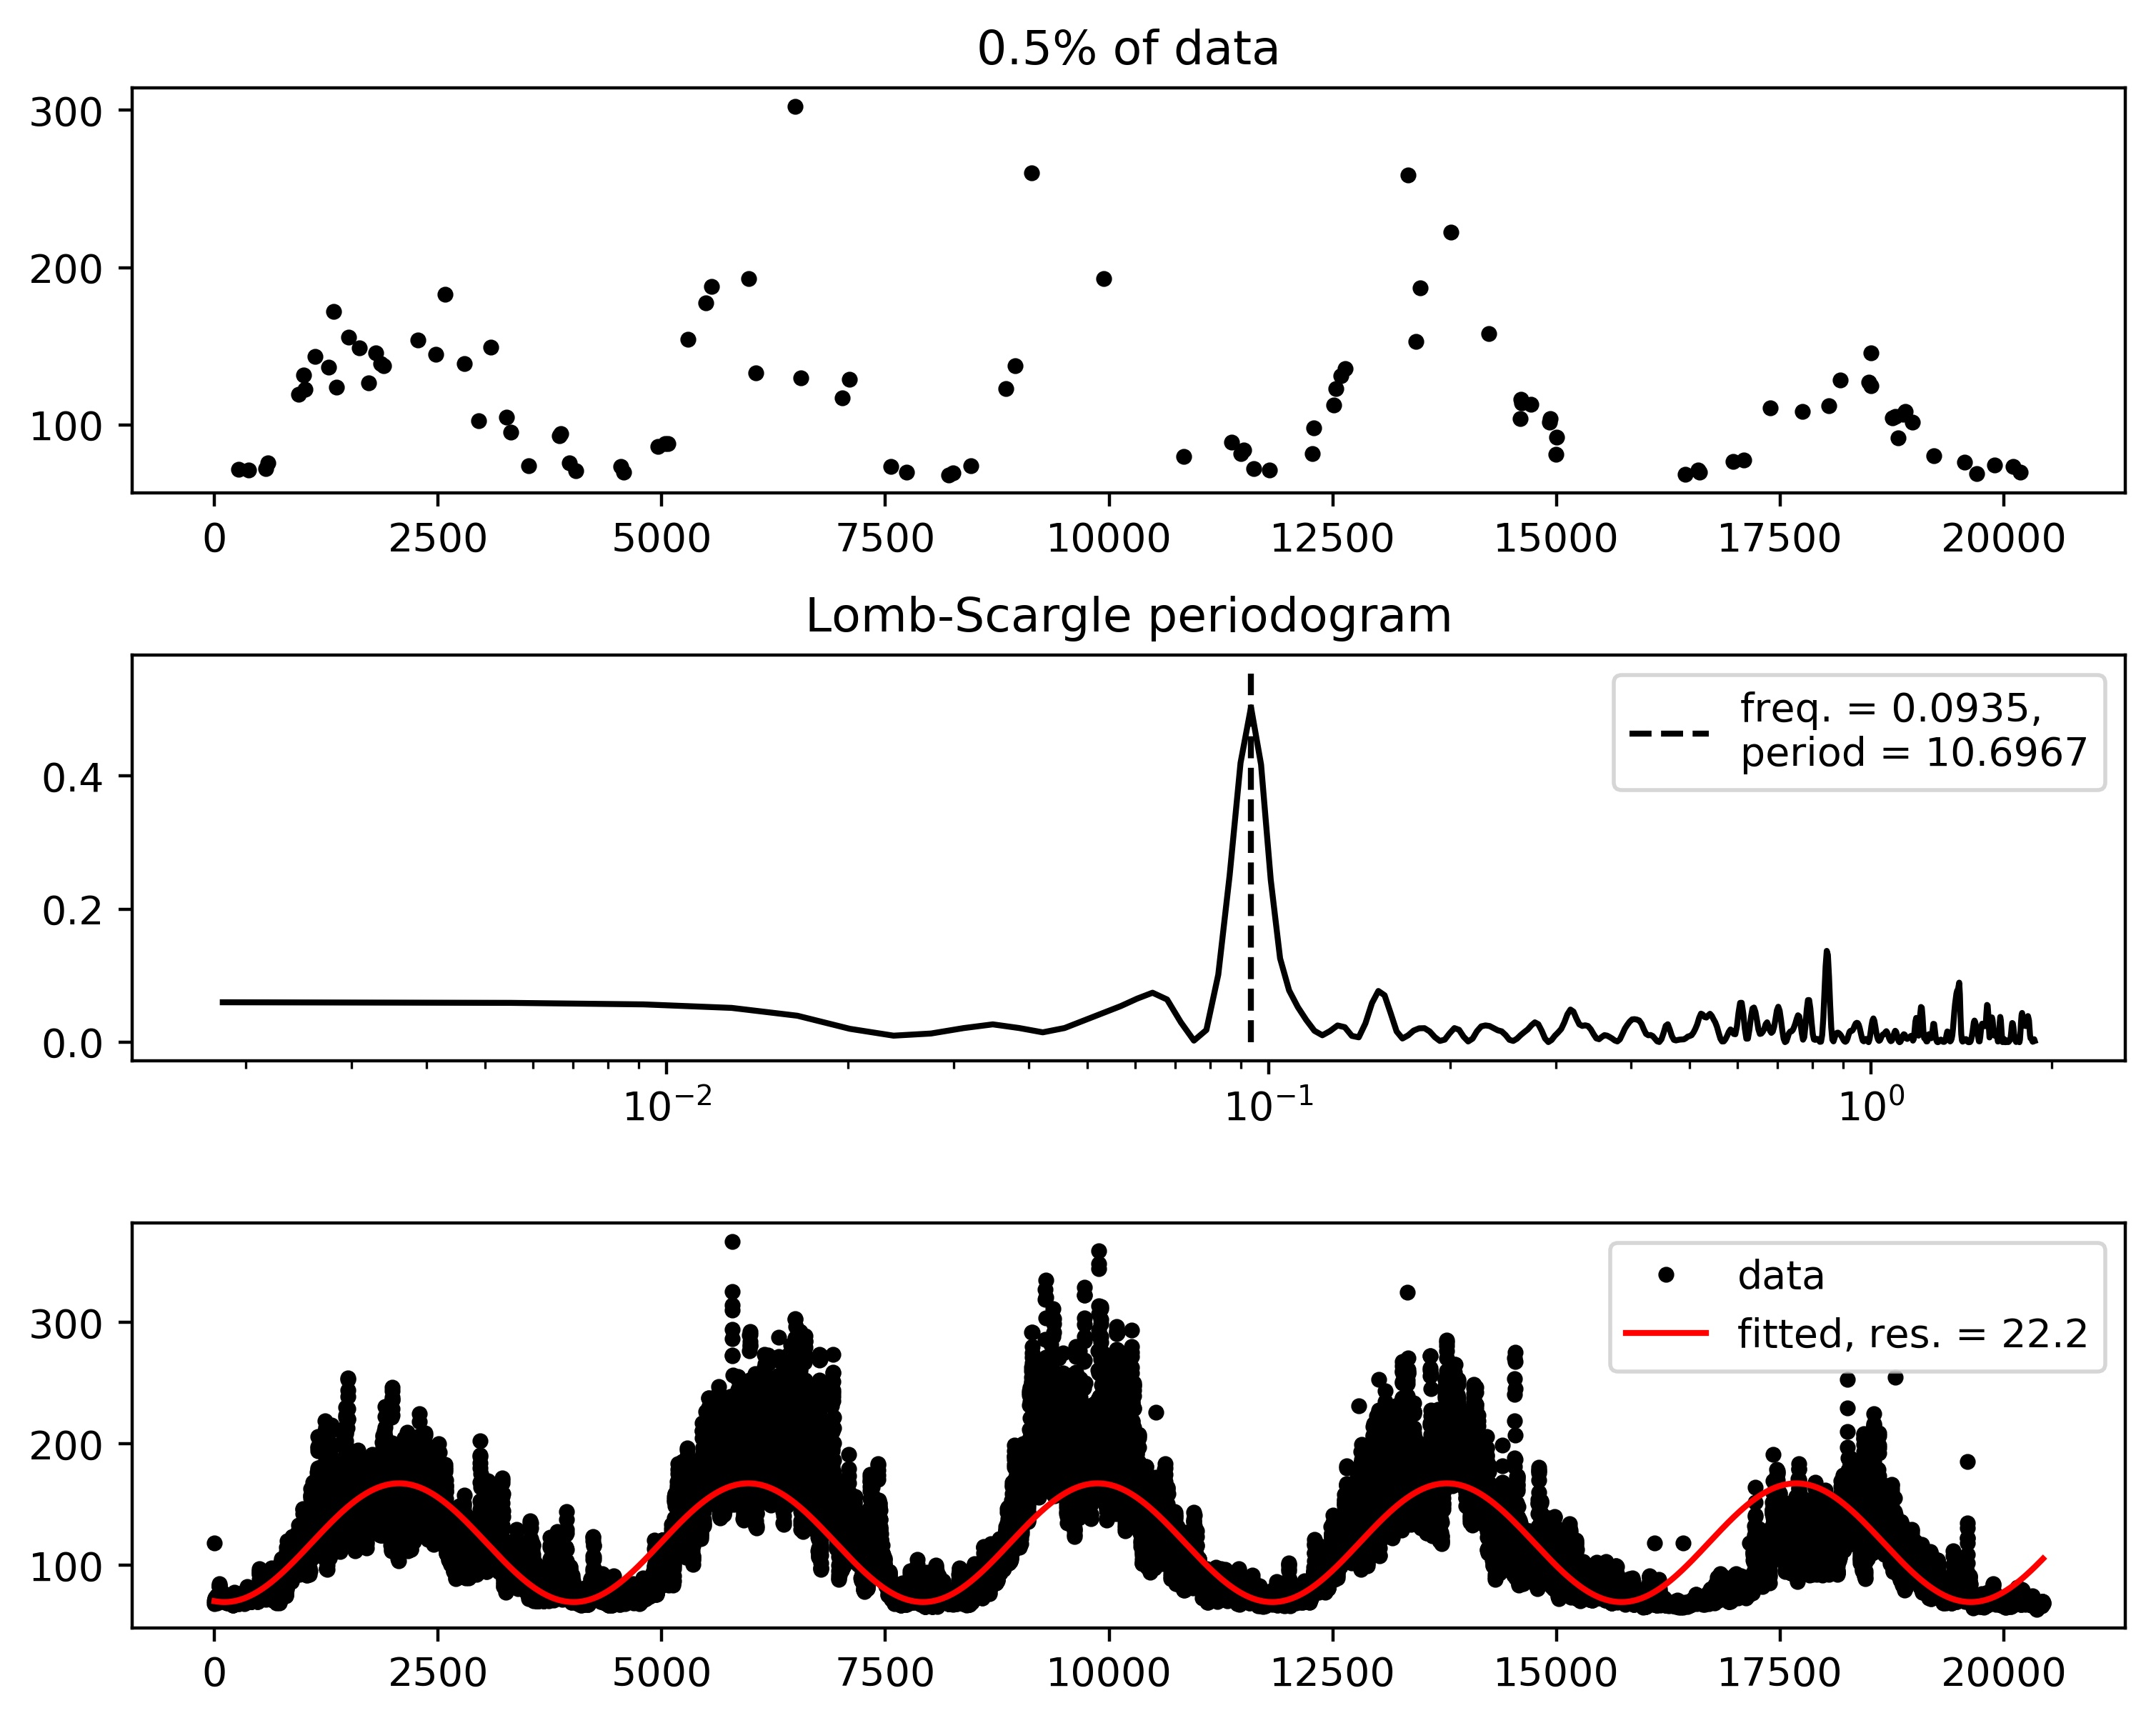
\includegraphics[scale=0.55]{../scripts/dataset1/periodograms_ny2.0_model1_pg0.995.jpg}
\end{center}
\end{frame}
\begin{frame}
\frametitle{Scenario 2 - daily averages}
\begin{center}
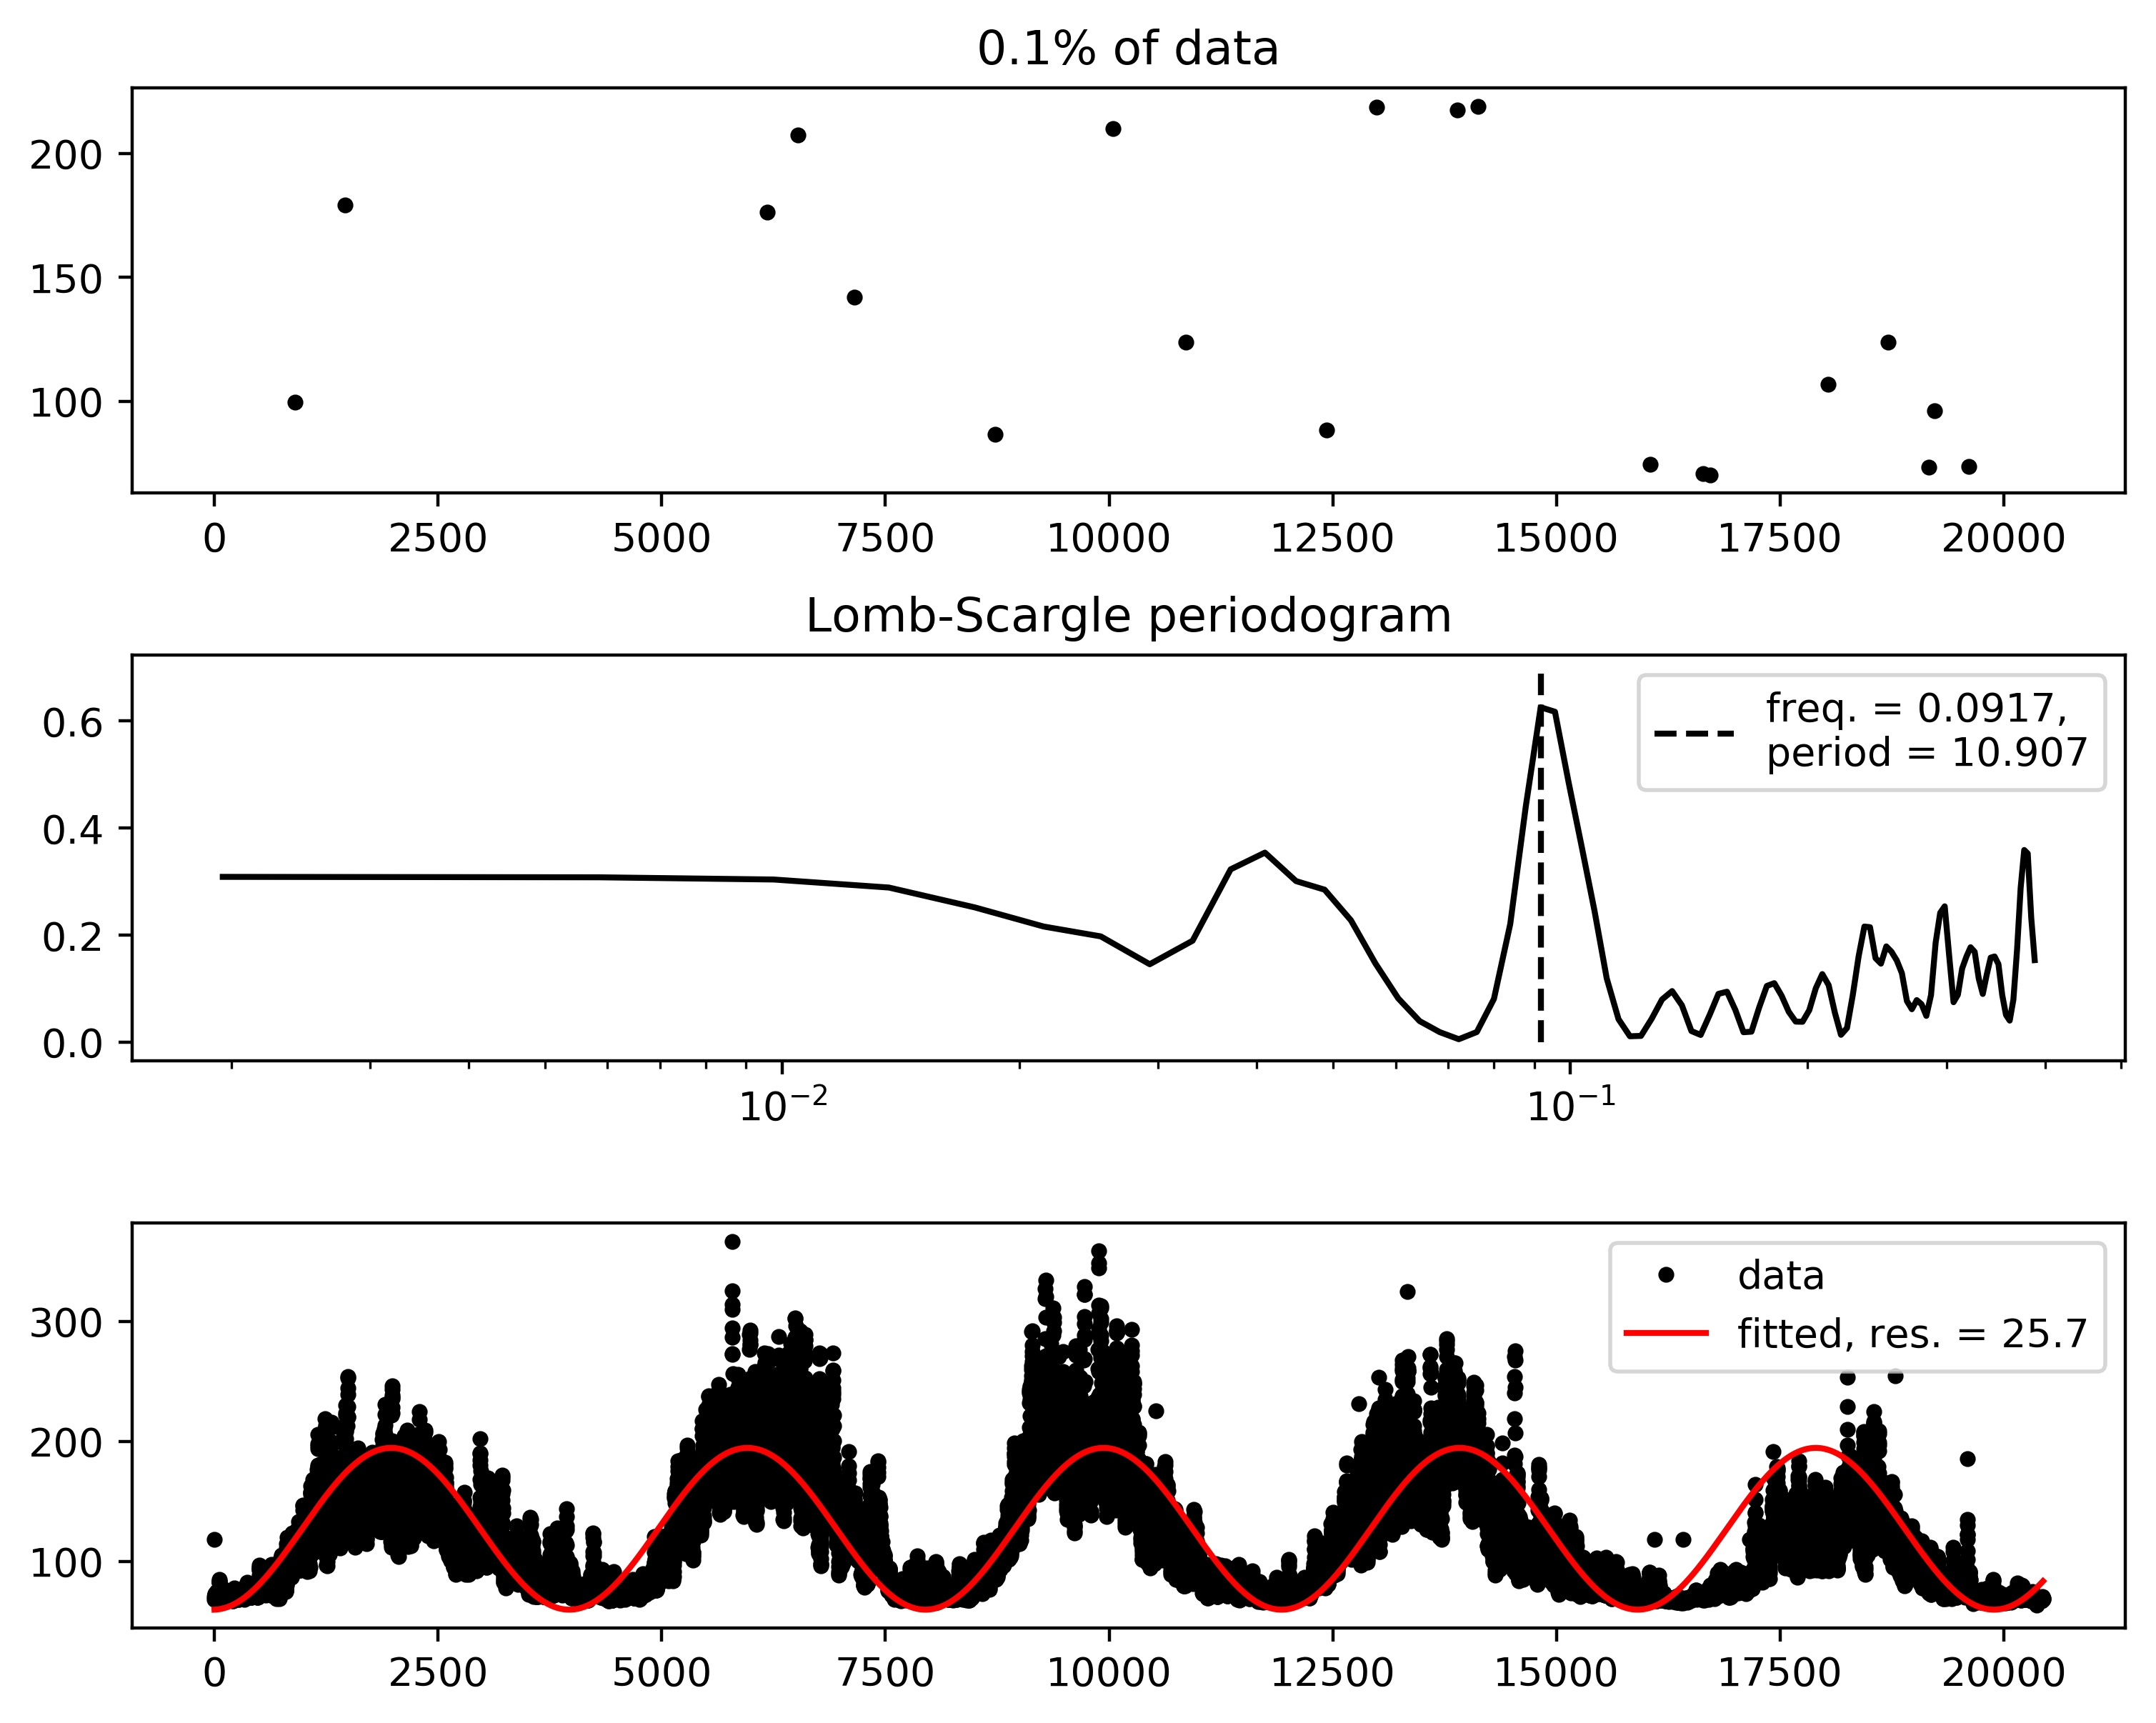
\includegraphics[scale=0.55]{../scripts/dataset1/periodograms_ny2.0_model1_pg0.999.jpg}
\end{center}
\end{frame}
\begin{frame}
\frametitle{Scenario 2 - daily averages}
\begin{center}
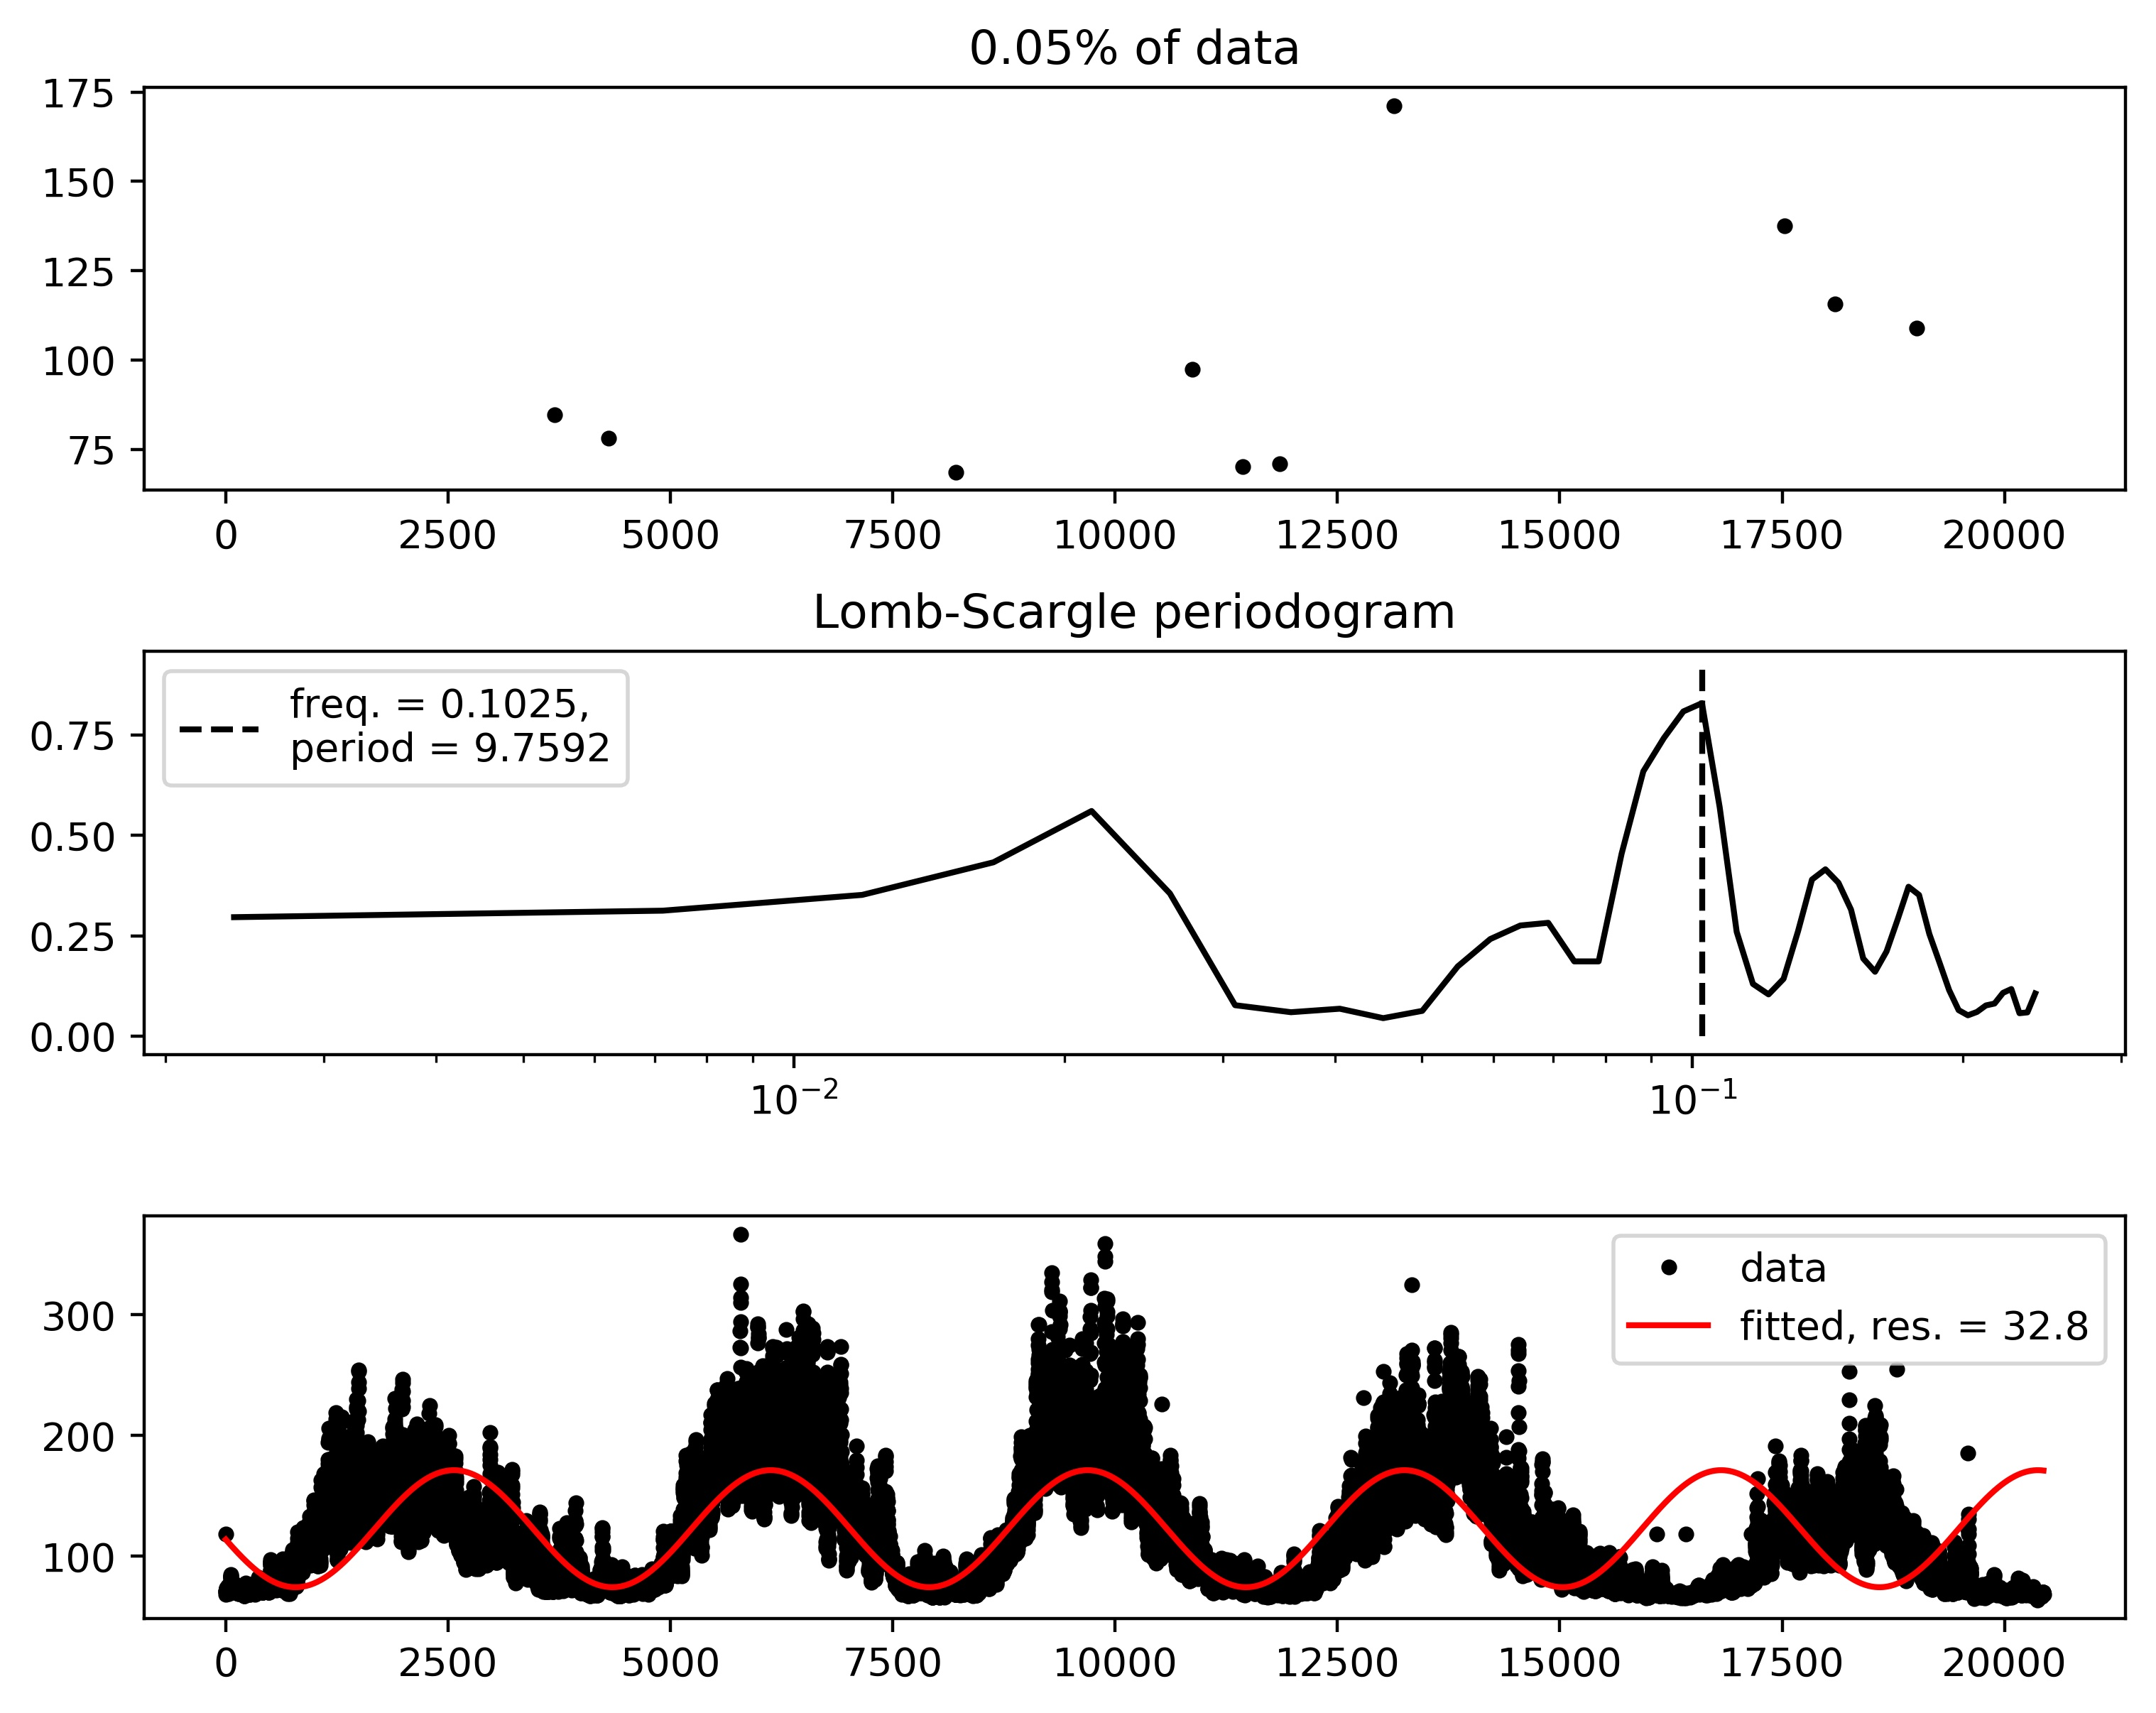
\includegraphics[scale=0.55]{../scripts/dataset1/periodograms_ny2.0_model1_pg0.9995.jpg}
\end{center}
\end{frame}
\begin{frame}
\frametitle{Scenario 2 - daily averages}
\begin{center}
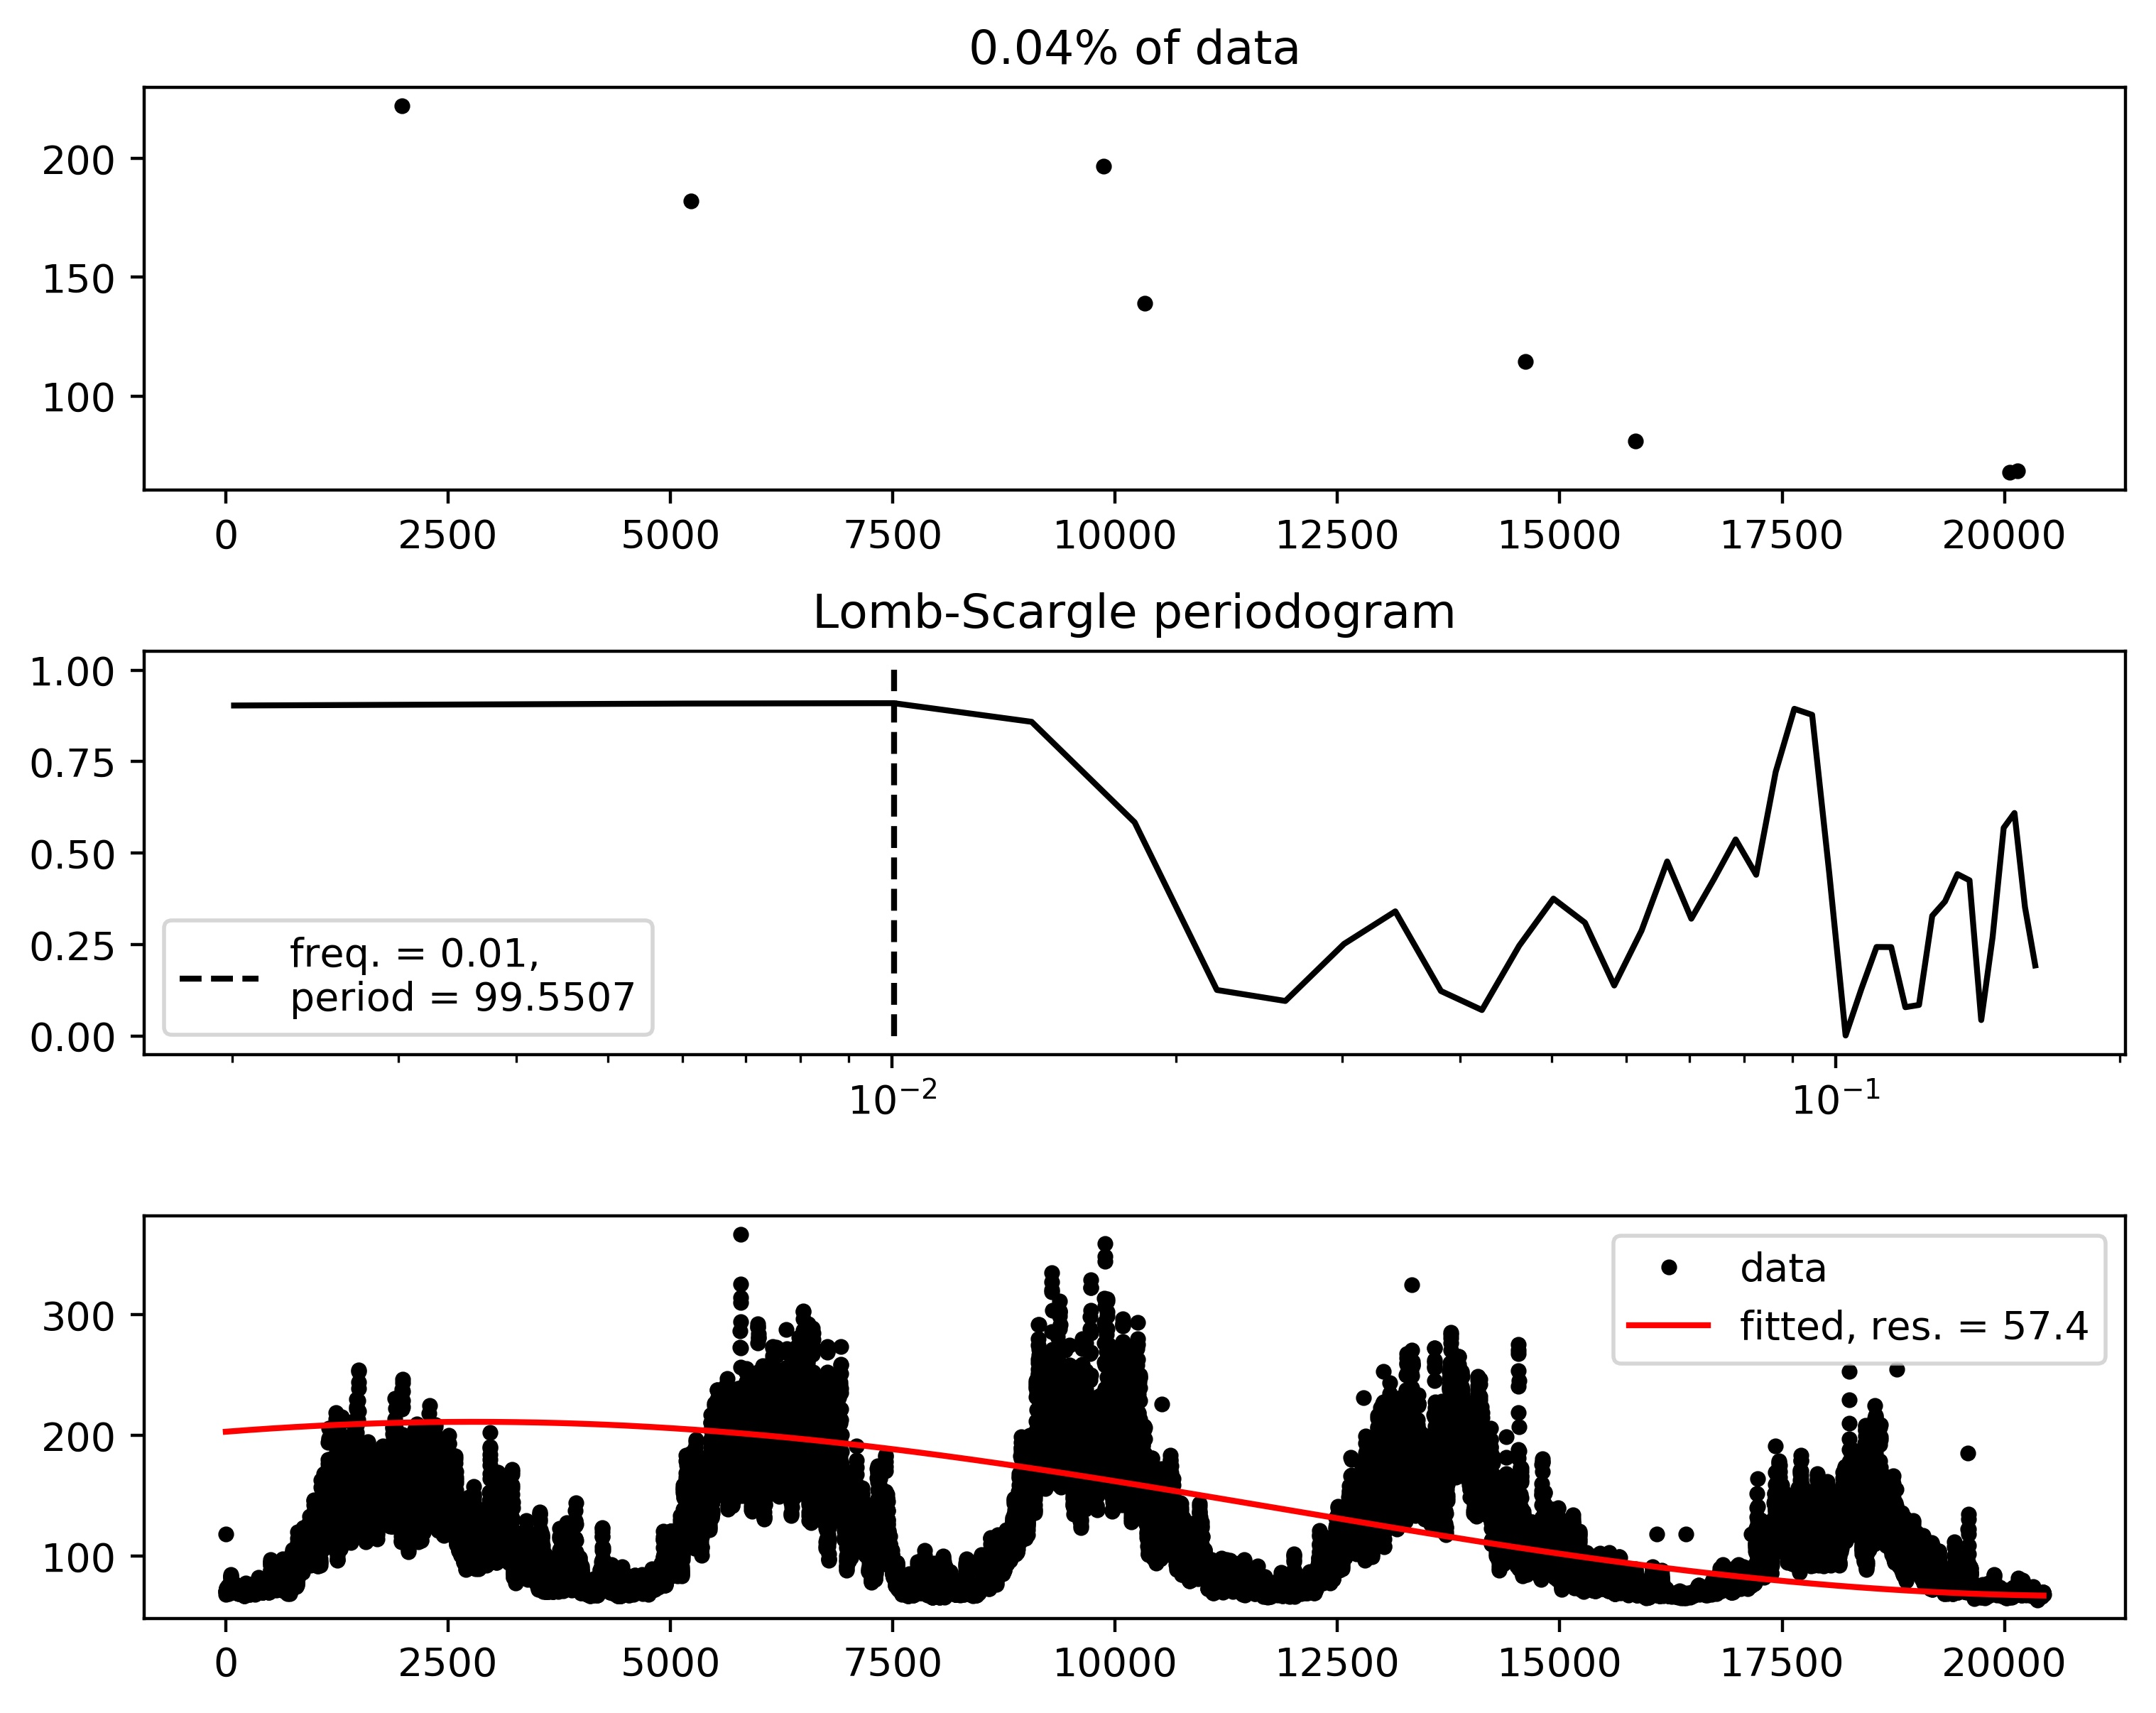
\includegraphics[scale=0.55]{../scripts/dataset1/periodograms_ny2.0_model1_pg0.9996.jpg}
\end{center}
\end{frame}

%%%%%%%%%%%%%%%%%%%%%%%%  FRAME  %%%%%%%%%%%%%%%%%%%%%%%%
\begin{frame}
\frametitle{Scenario 2 - 27-day averages}
\begin{center}
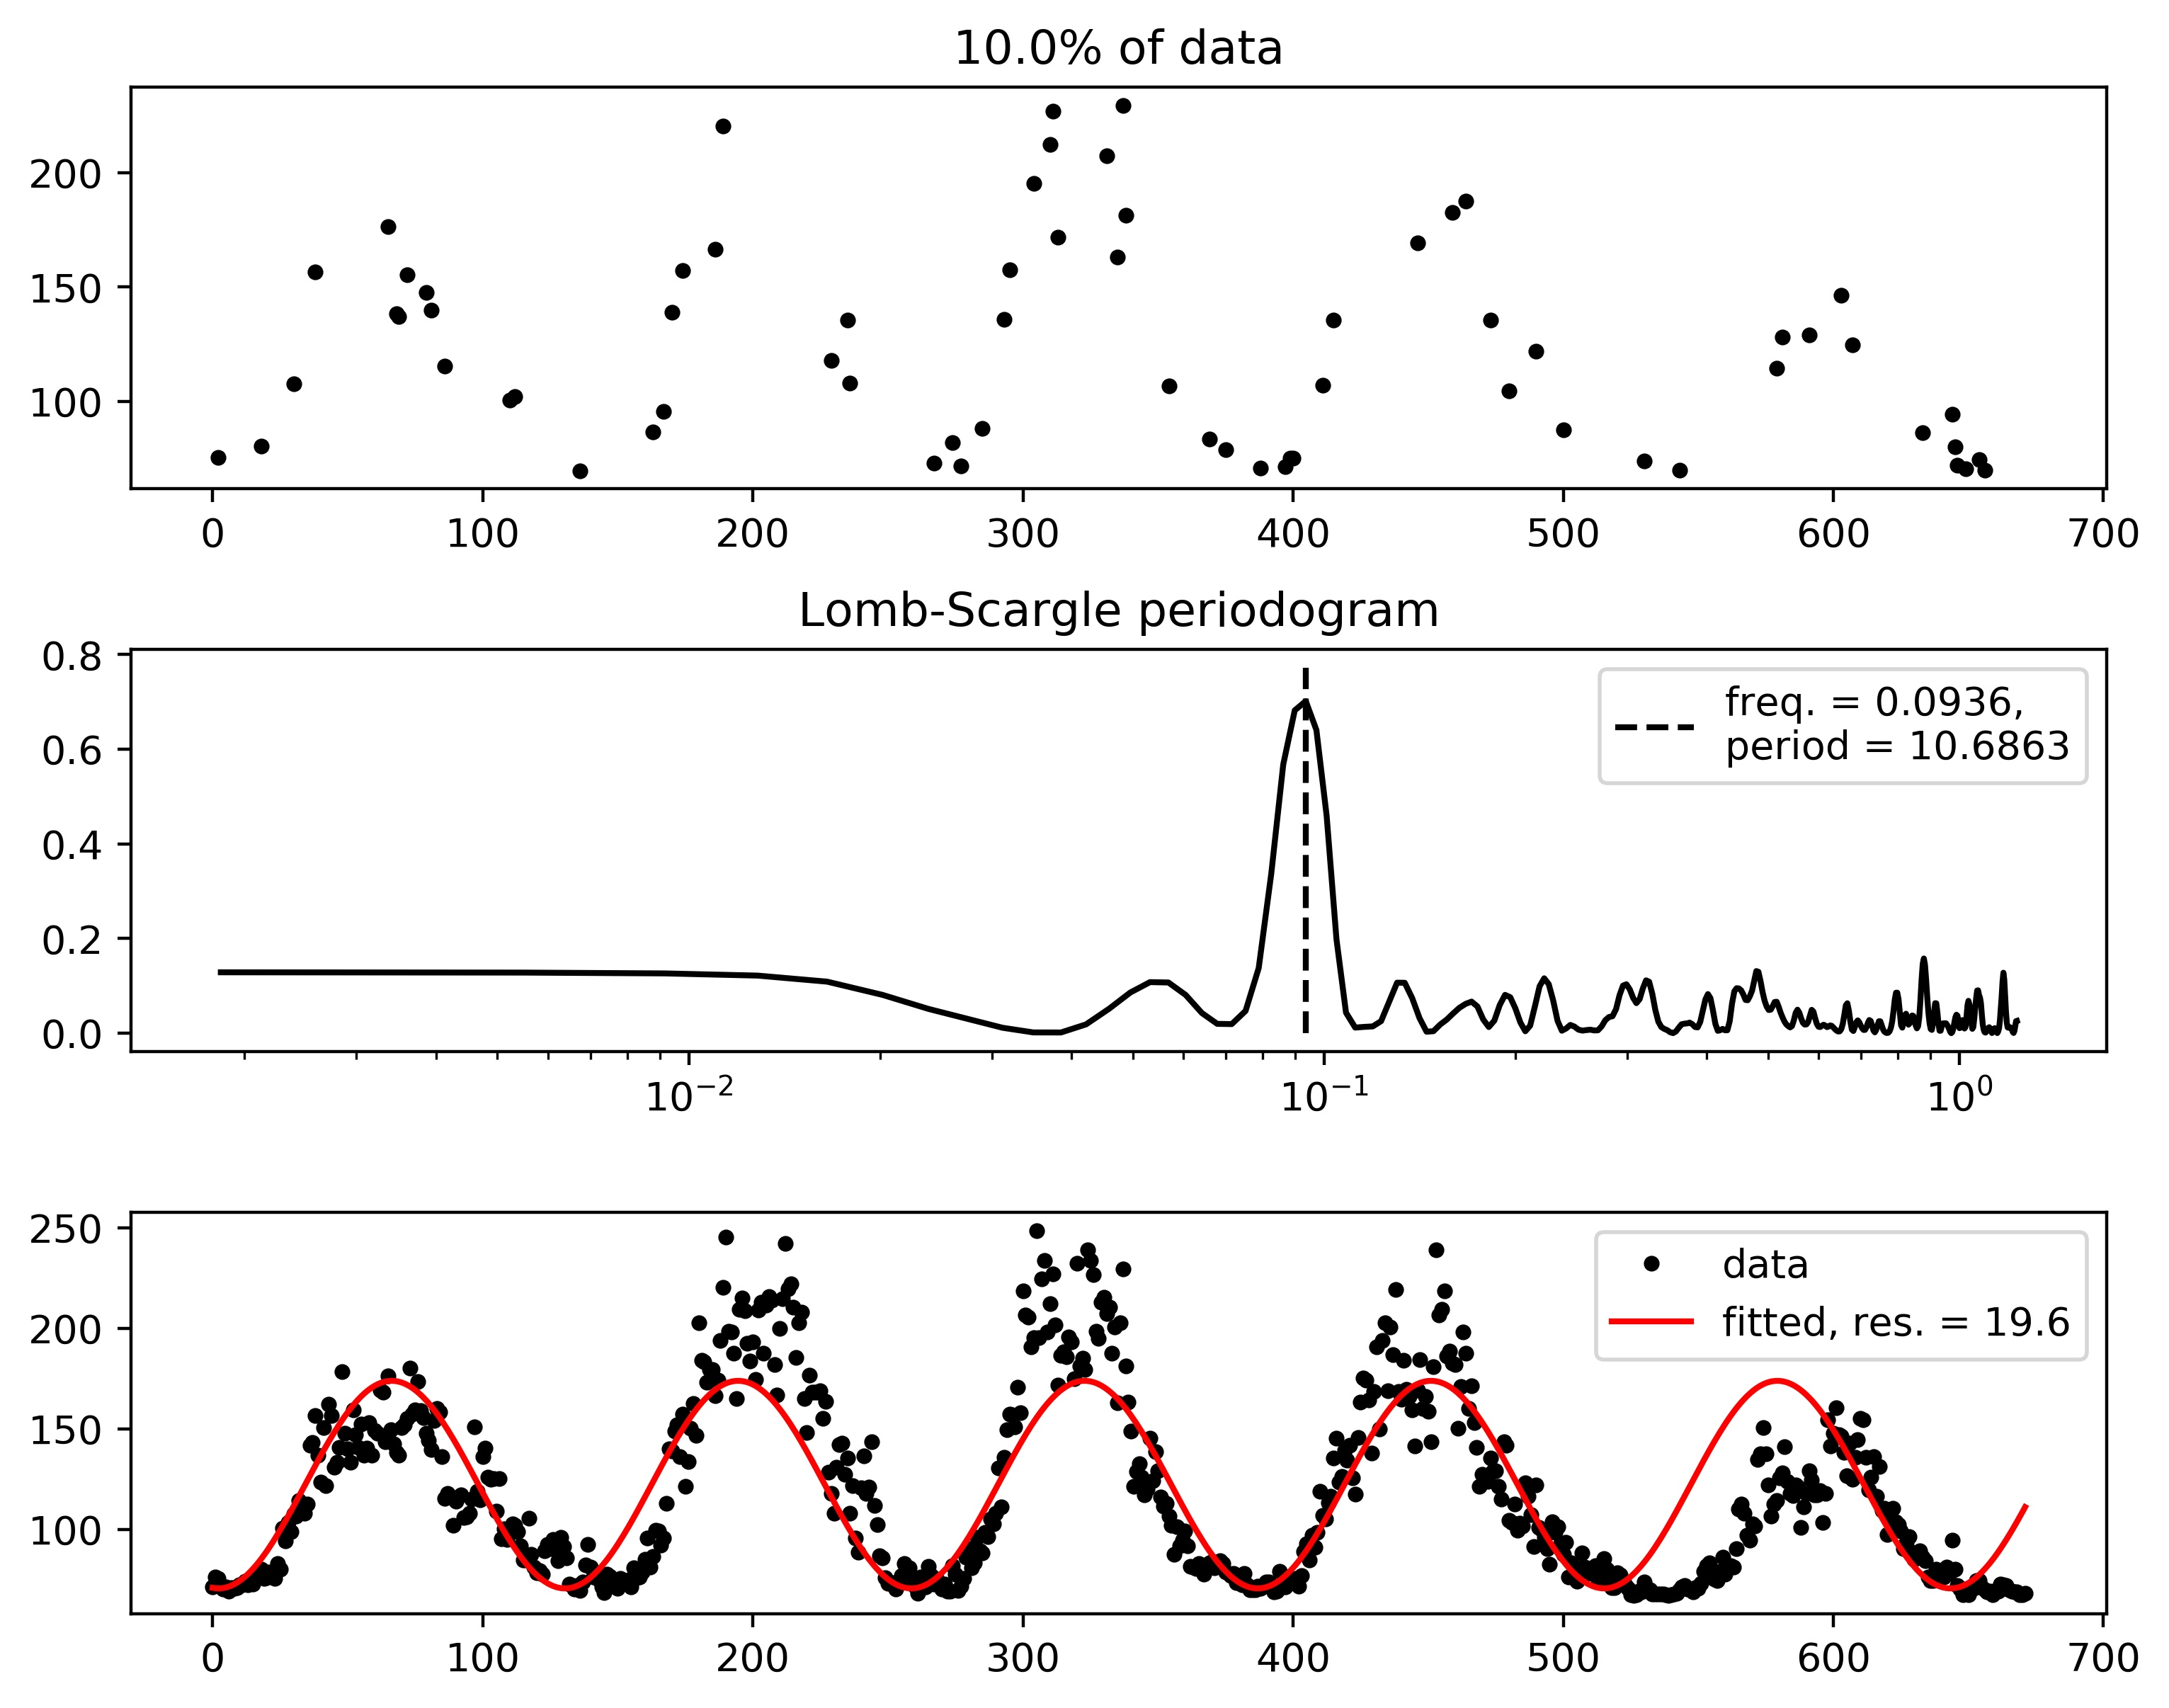
\includegraphics[scale=0.55]{../scripts/dataset2/periodograms_ny2.0_model1_pg0.9.jpg}
\end{center}
\end{frame}
\begin{frame}
\frametitle{Scenario 2 - 27-day averages}
\begin{center}
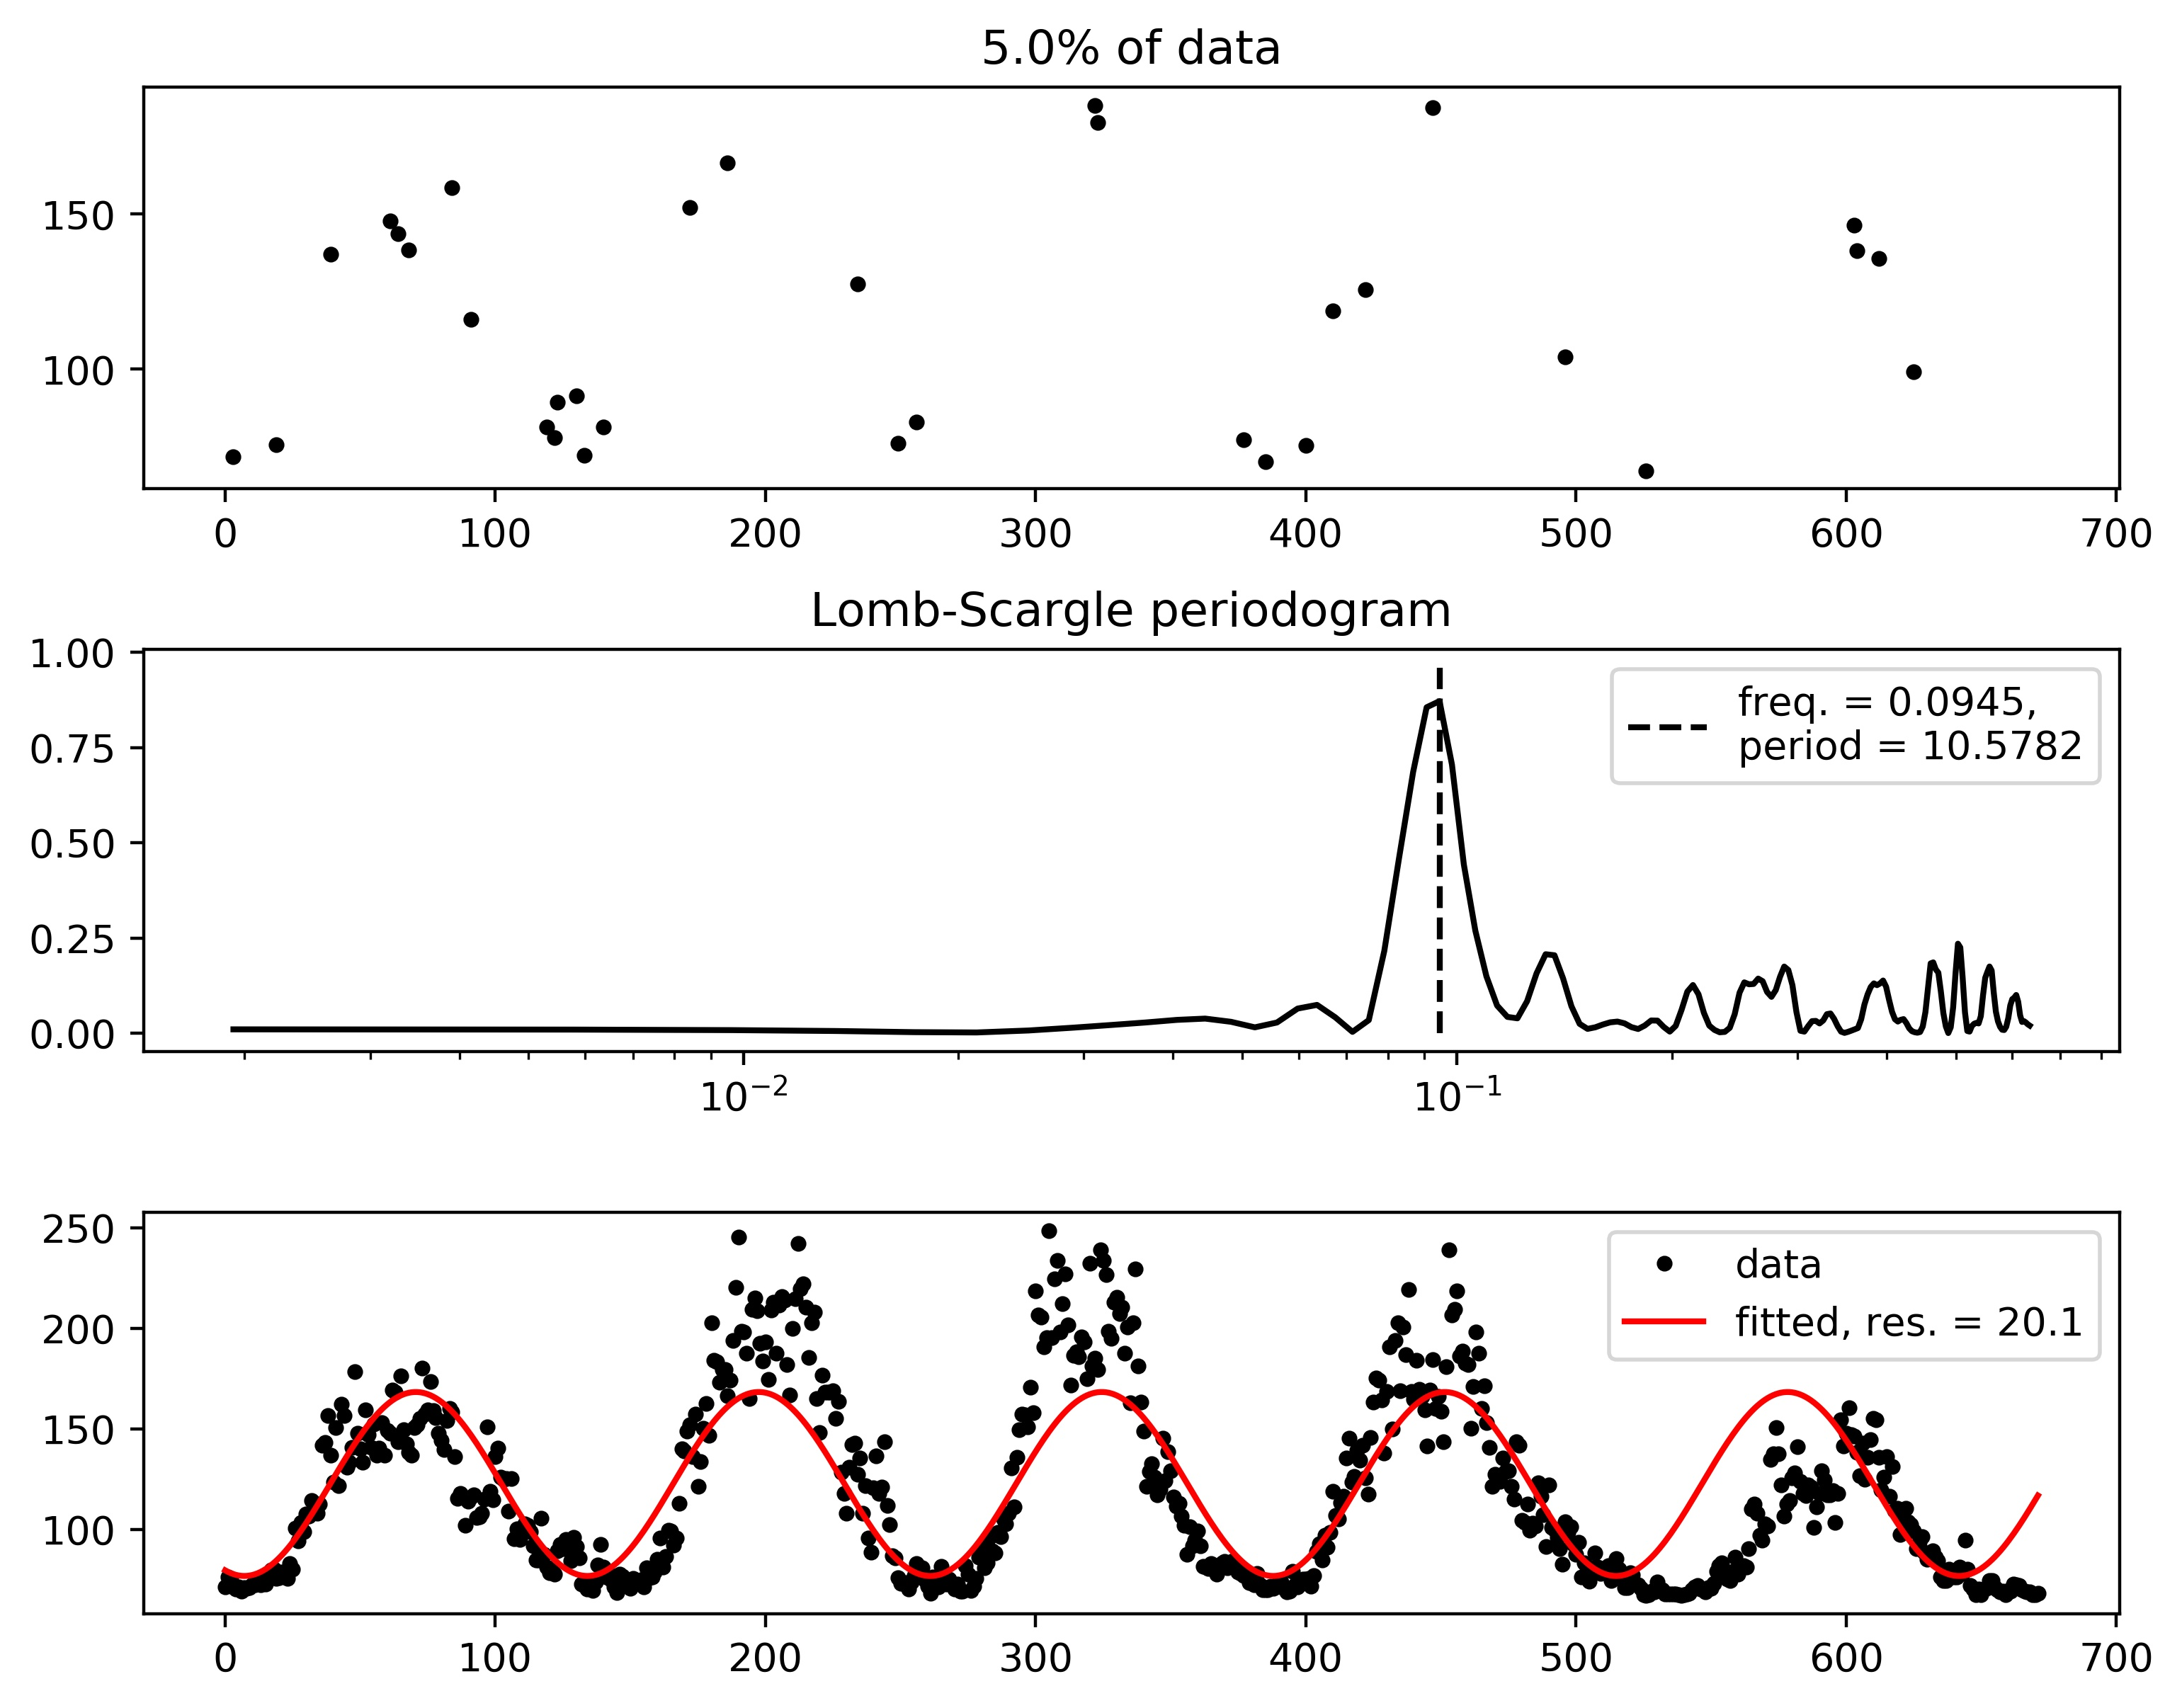
\includegraphics[scale=0.55]{../scripts/dataset2/periodograms_ny2.0_model1_pg0.95.jpg}
\end{center}
\end{frame}
\begin{frame}
\frametitle{Scenario 2 - 27-day averages}
\begin{center}
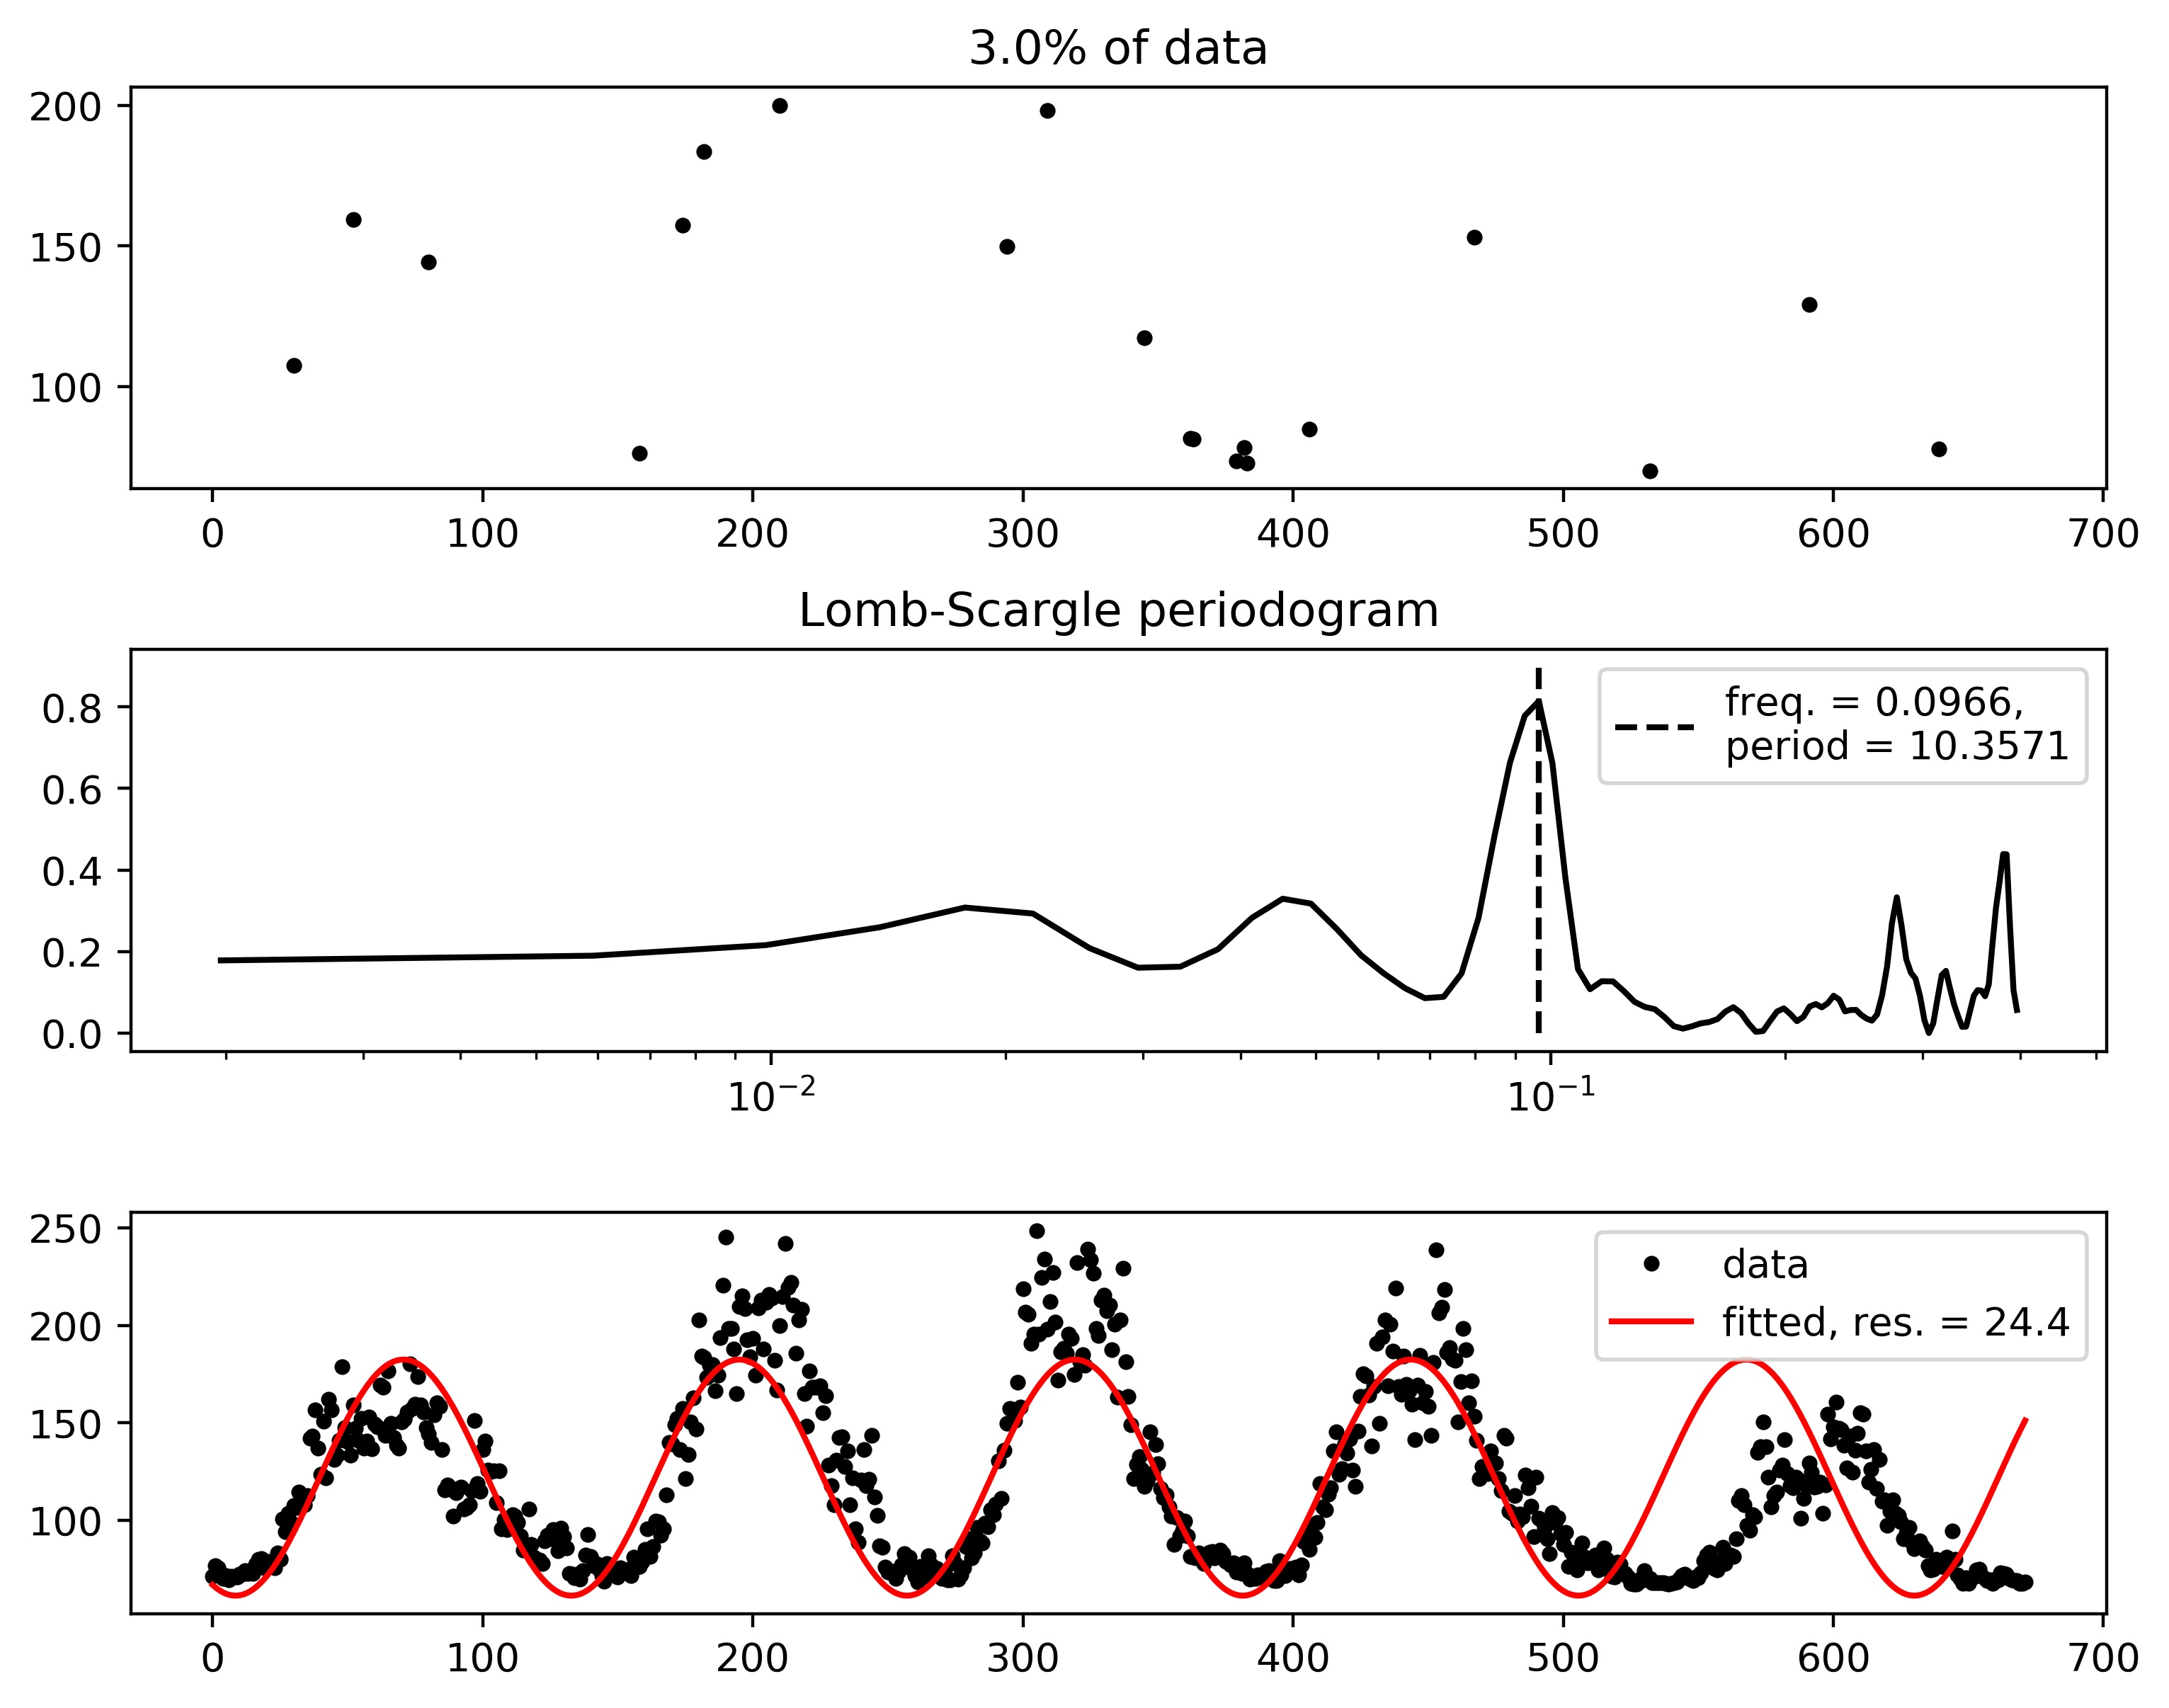
\includegraphics[scale=0.55]{../scripts/dataset2/periodograms_ny2.0_model1_pg0.97.jpg}
\end{center}
\end{frame}
\begin{frame}
\frametitle{Scenario 2 - 27-day averages}
\begin{center}
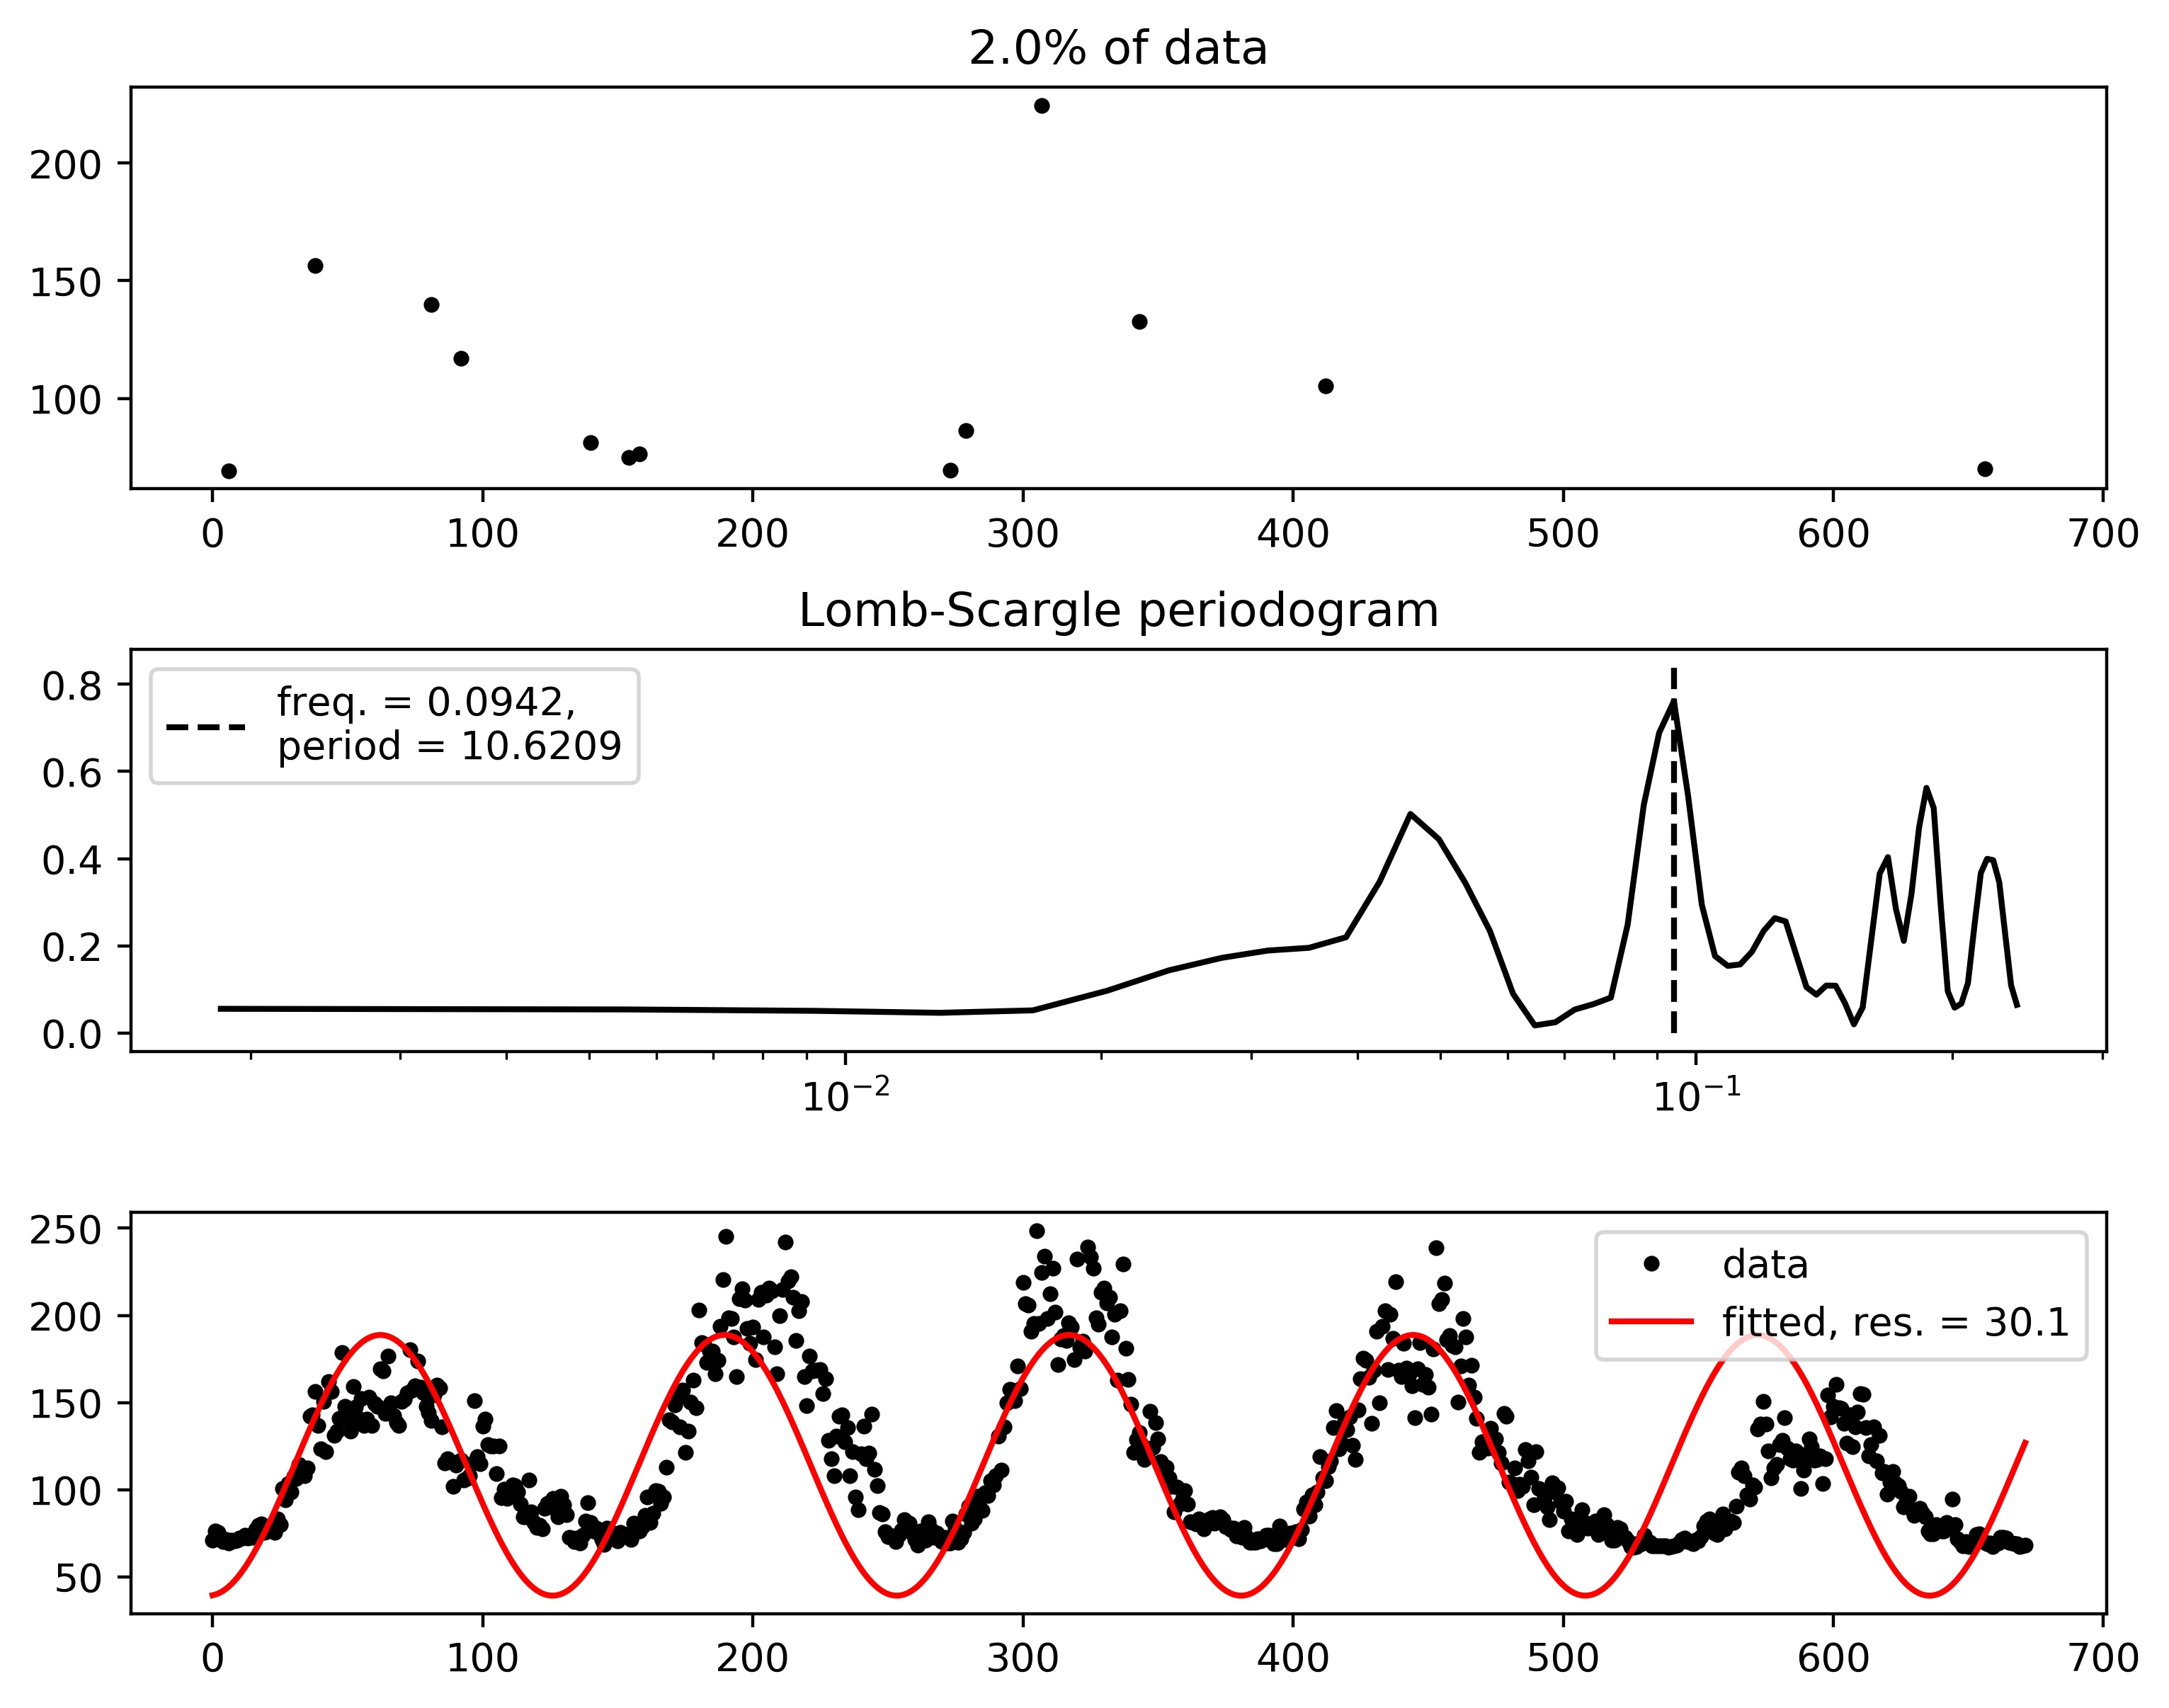
\includegraphics[scale=0.55]{../scripts/dataset2/periodograms_ny2.0_model1_pg0.98.jpg}
\end{center}
\end{frame}
\begin{frame}
\frametitle{Scenario 2 - 27-day averages}
\begin{center}
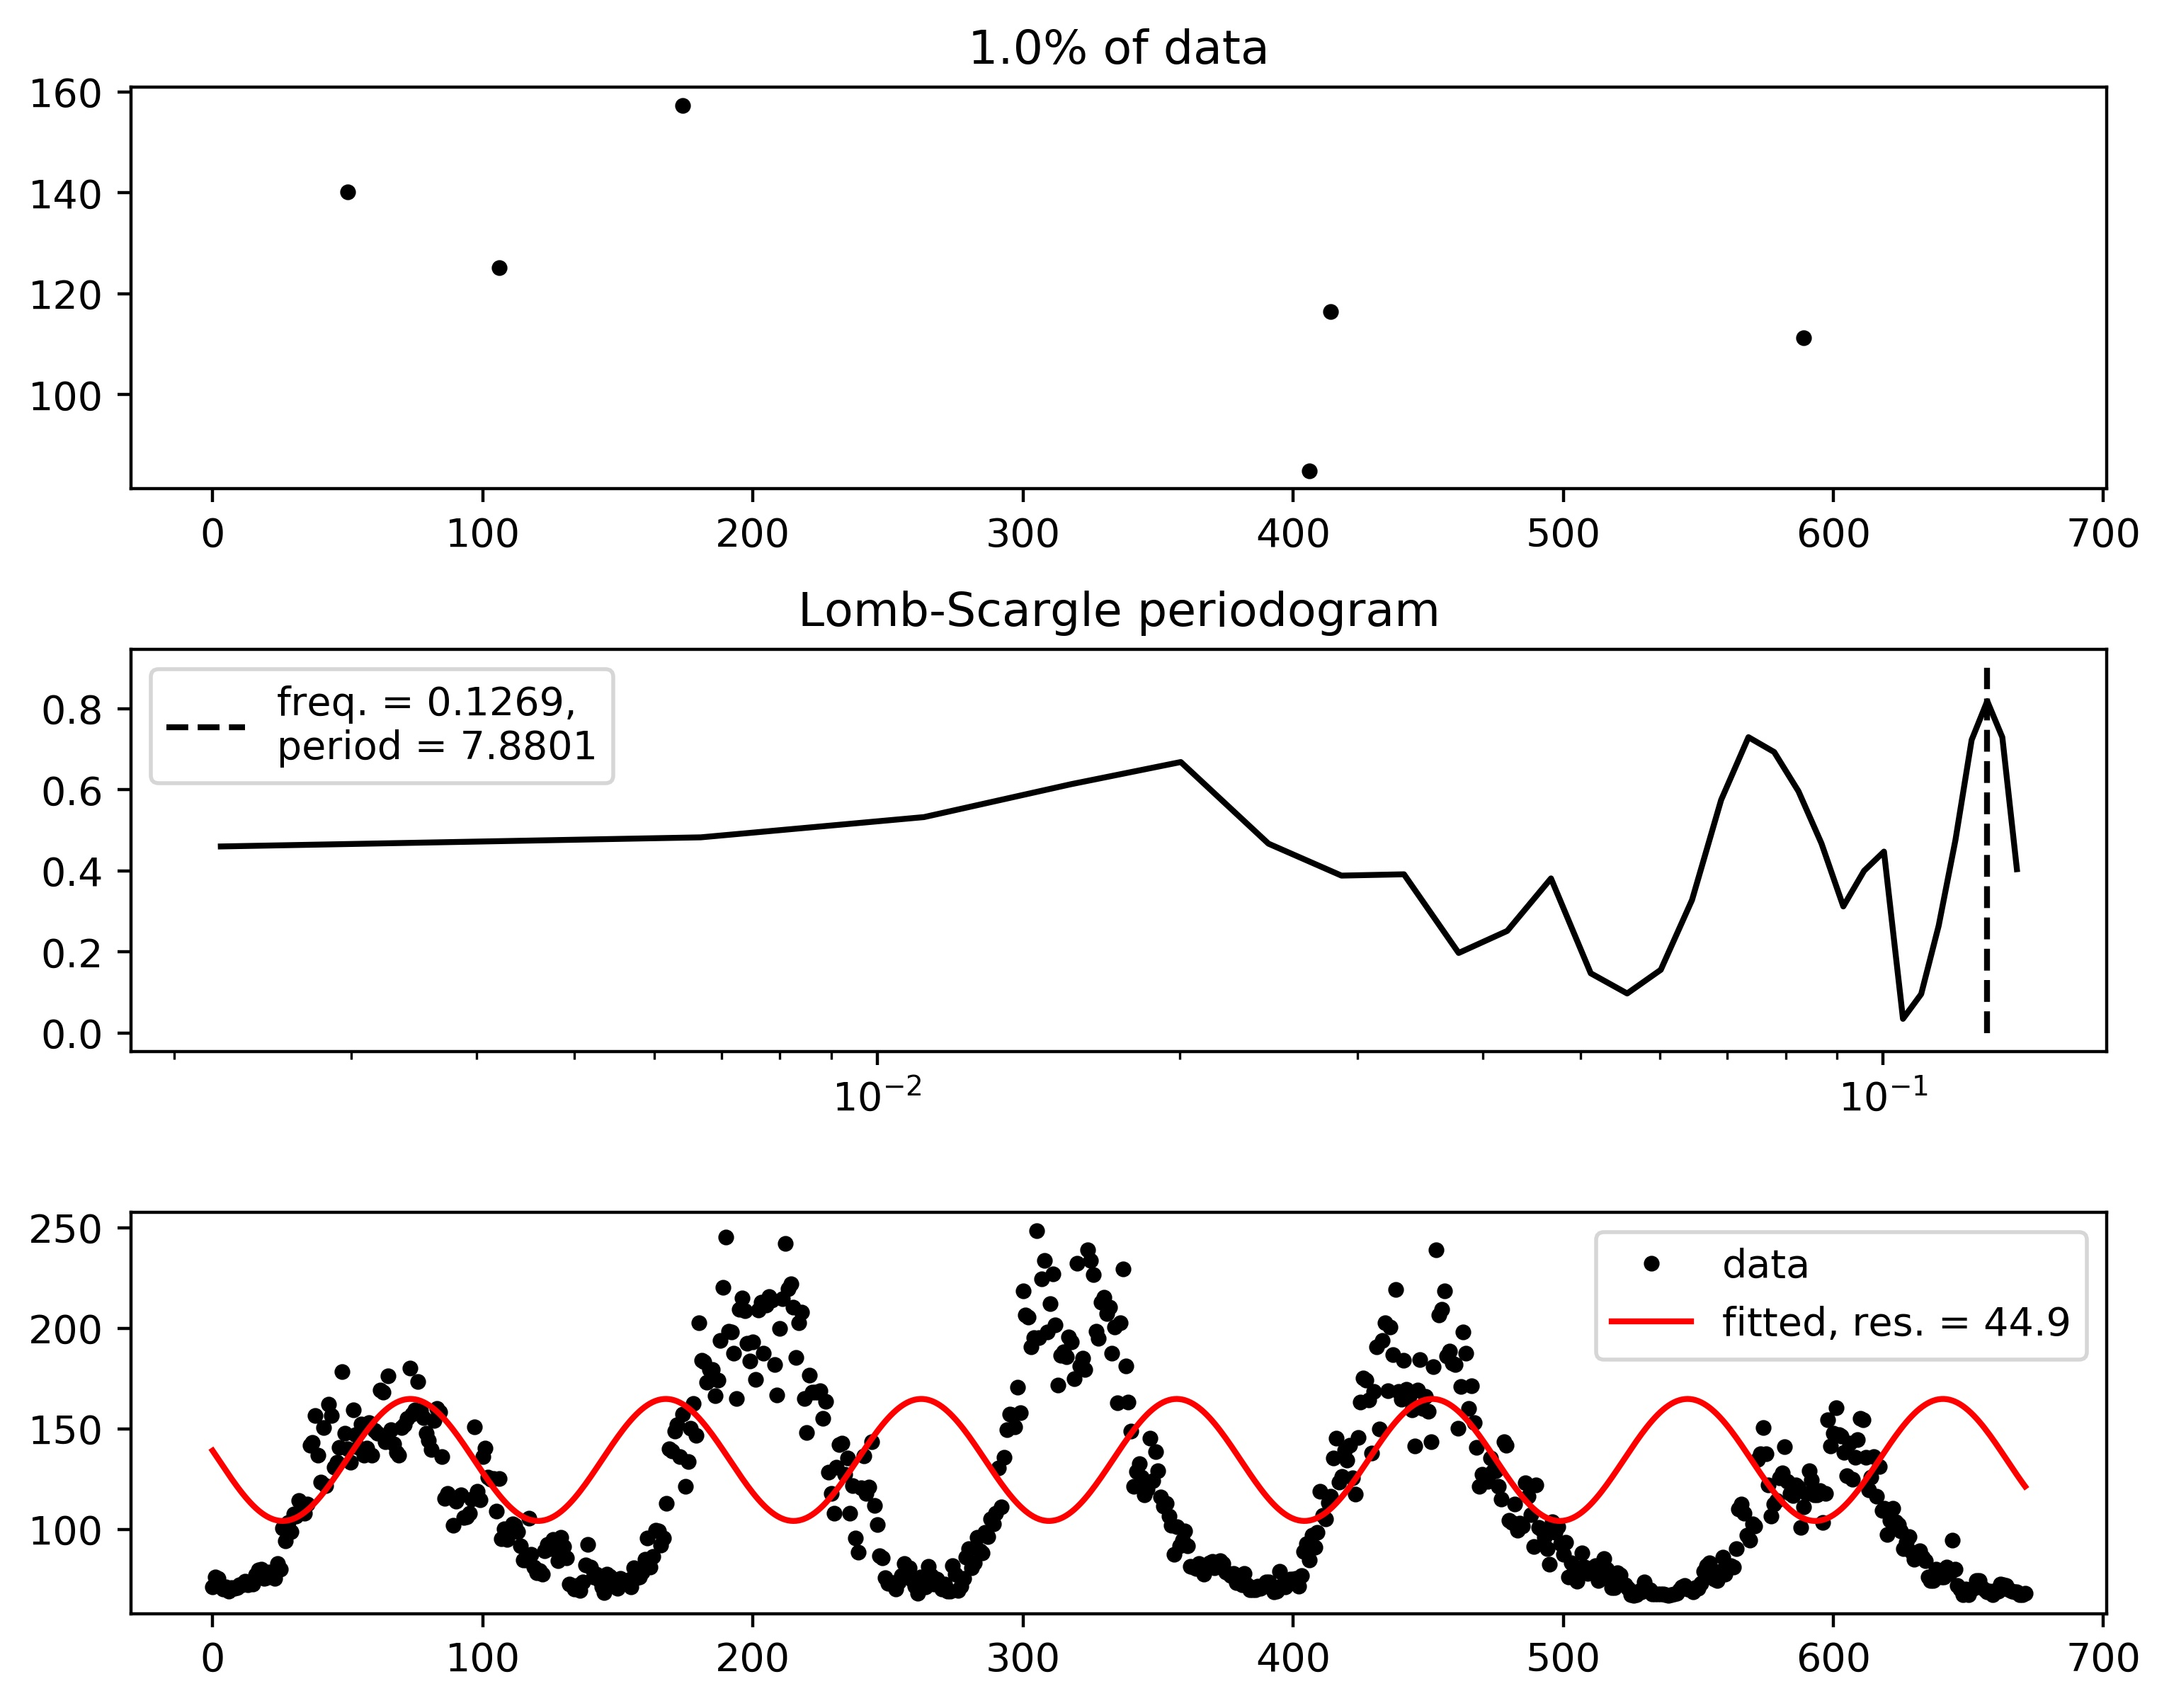
\includegraphics[scale=0.55]{../scripts/dataset2/periodograms_ny2.0_model1_pg0.99.jpg}
\end{center}
\end{frame}

%%%%%%%%%%%%%%%%%%%%%%%%  FRAME  %%%%%%%%%%%%%%%%%%%%%%%%
\begin{frame}
\frametitle{Scenario 2 - yearly averages}
\begin{center}
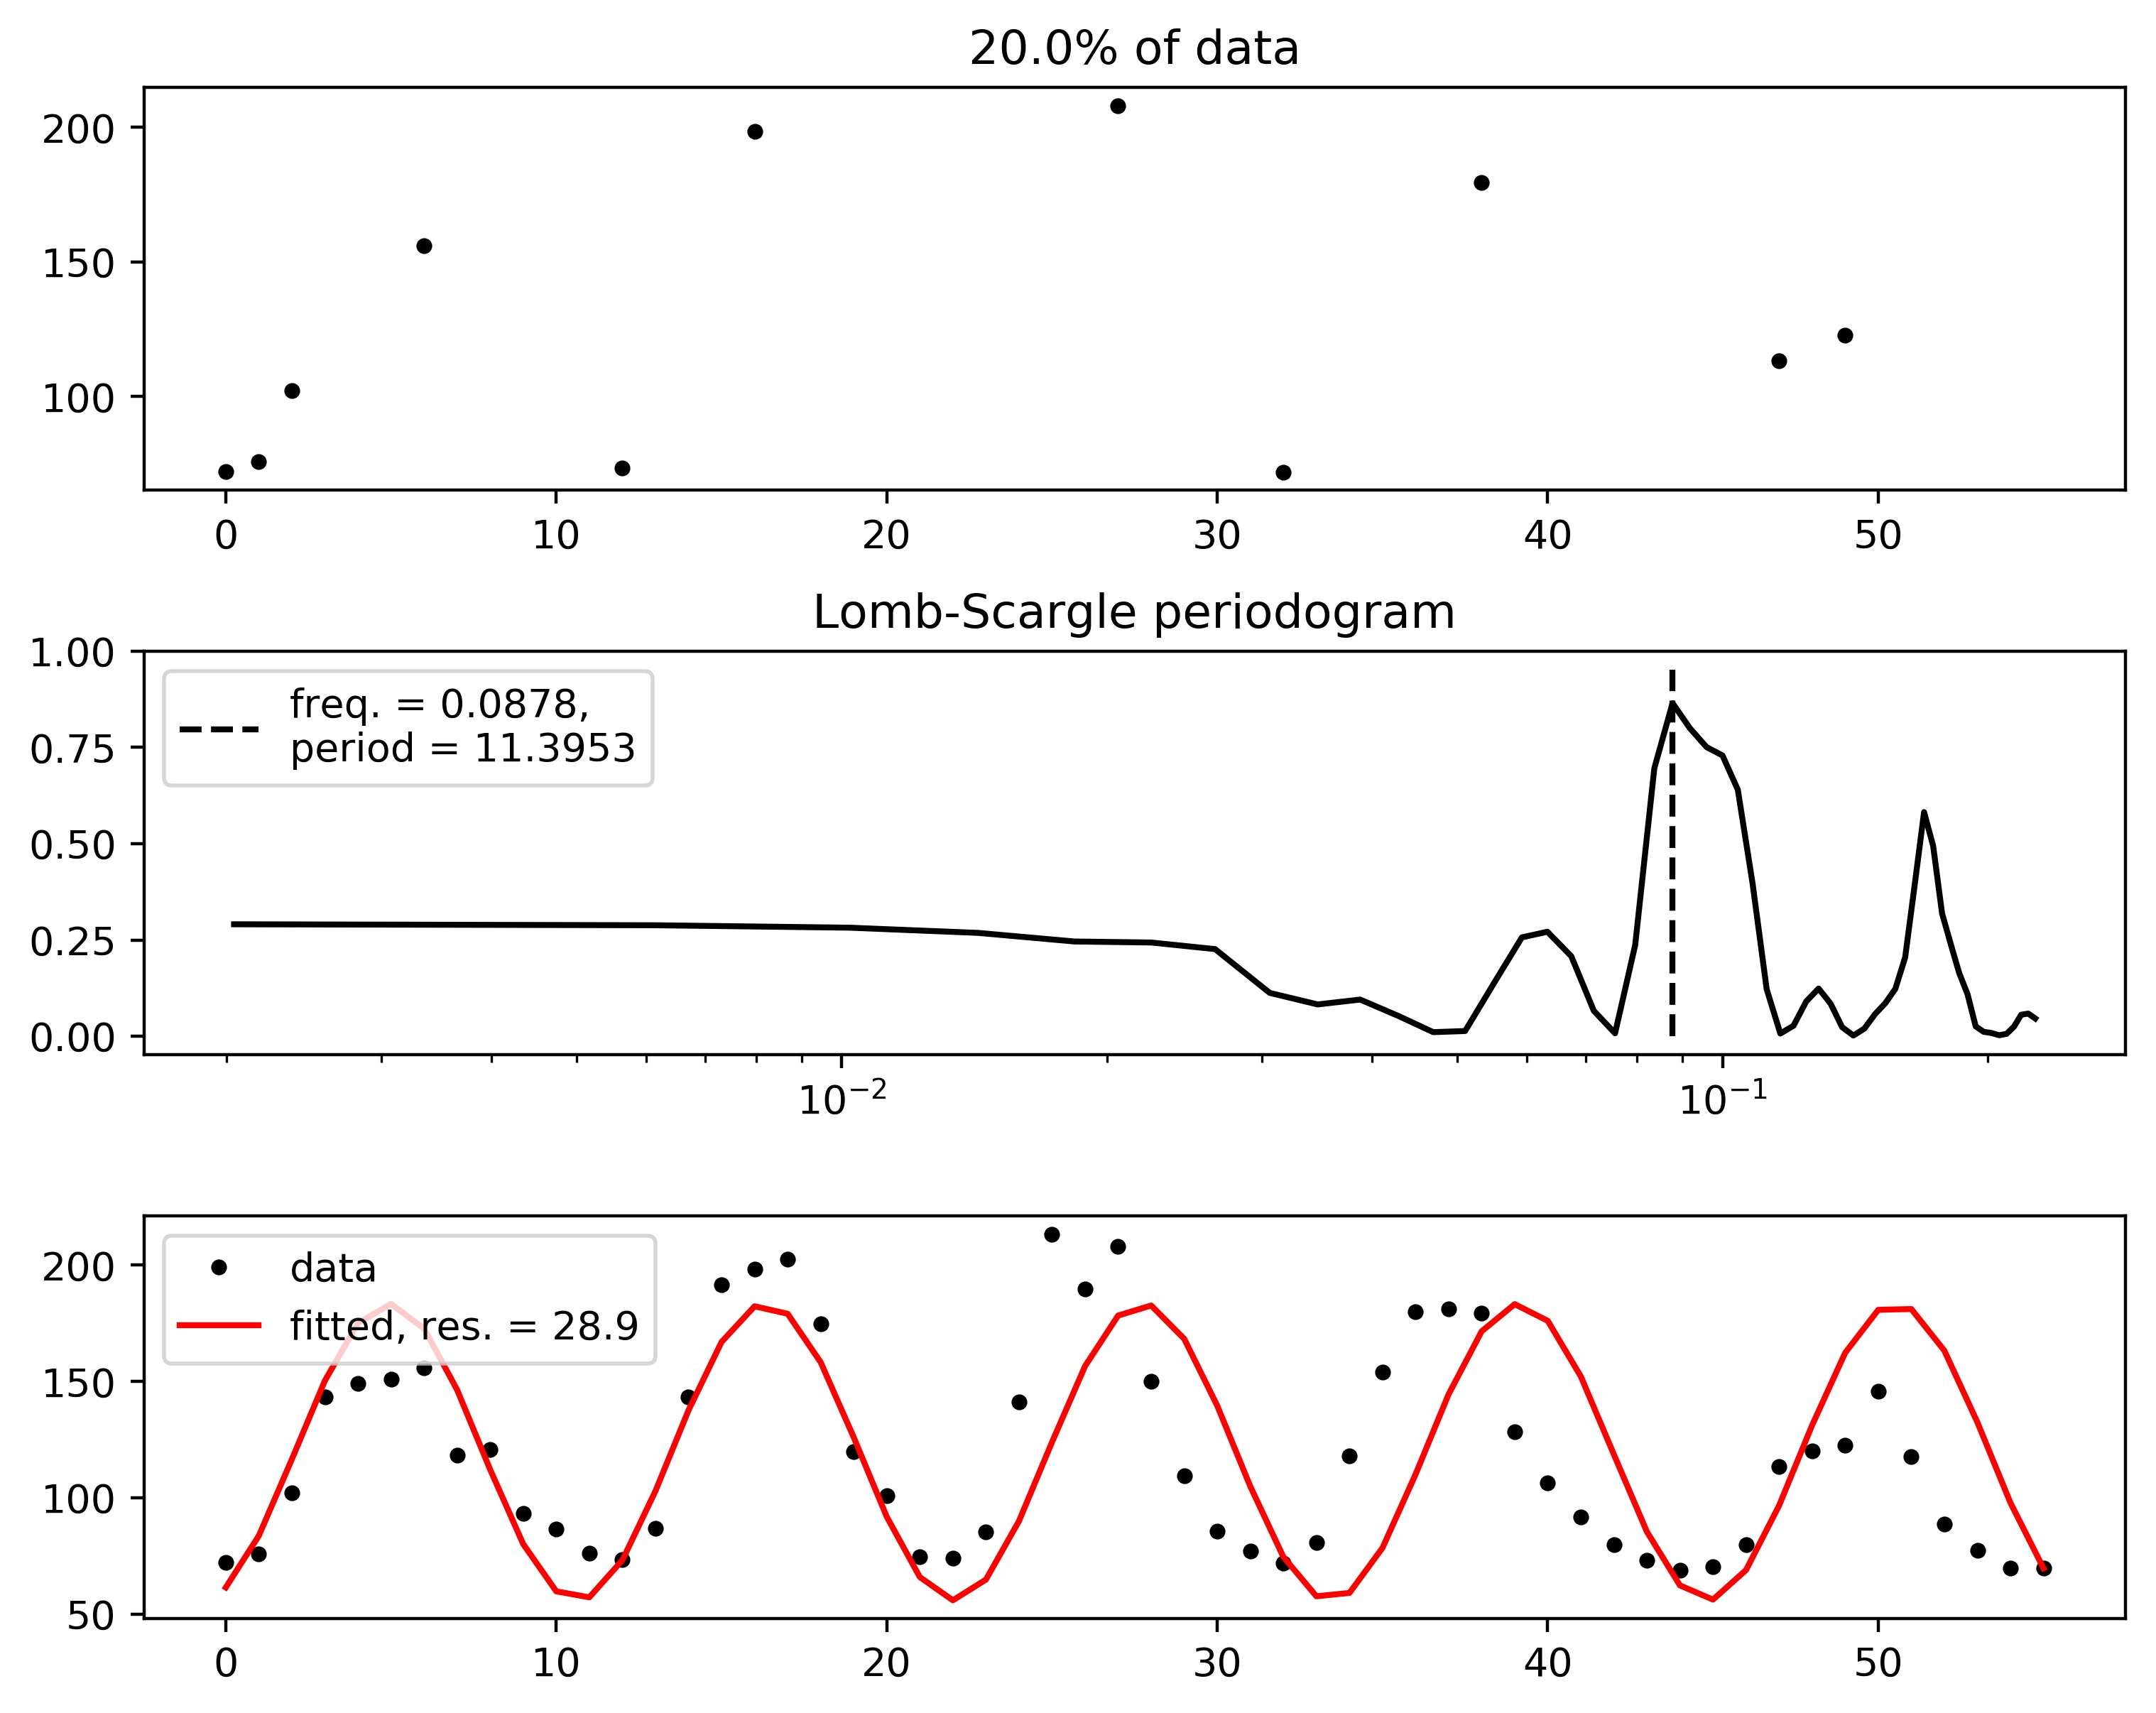
\includegraphics[scale=0.55]{../scripts/dataset3/periodograms_ny2.0_model1_pg0.8.jpg}
\end{center}
\end{frame}
\begin{frame}
\frametitle{Scenario 2 - yearly averages}
\begin{center}
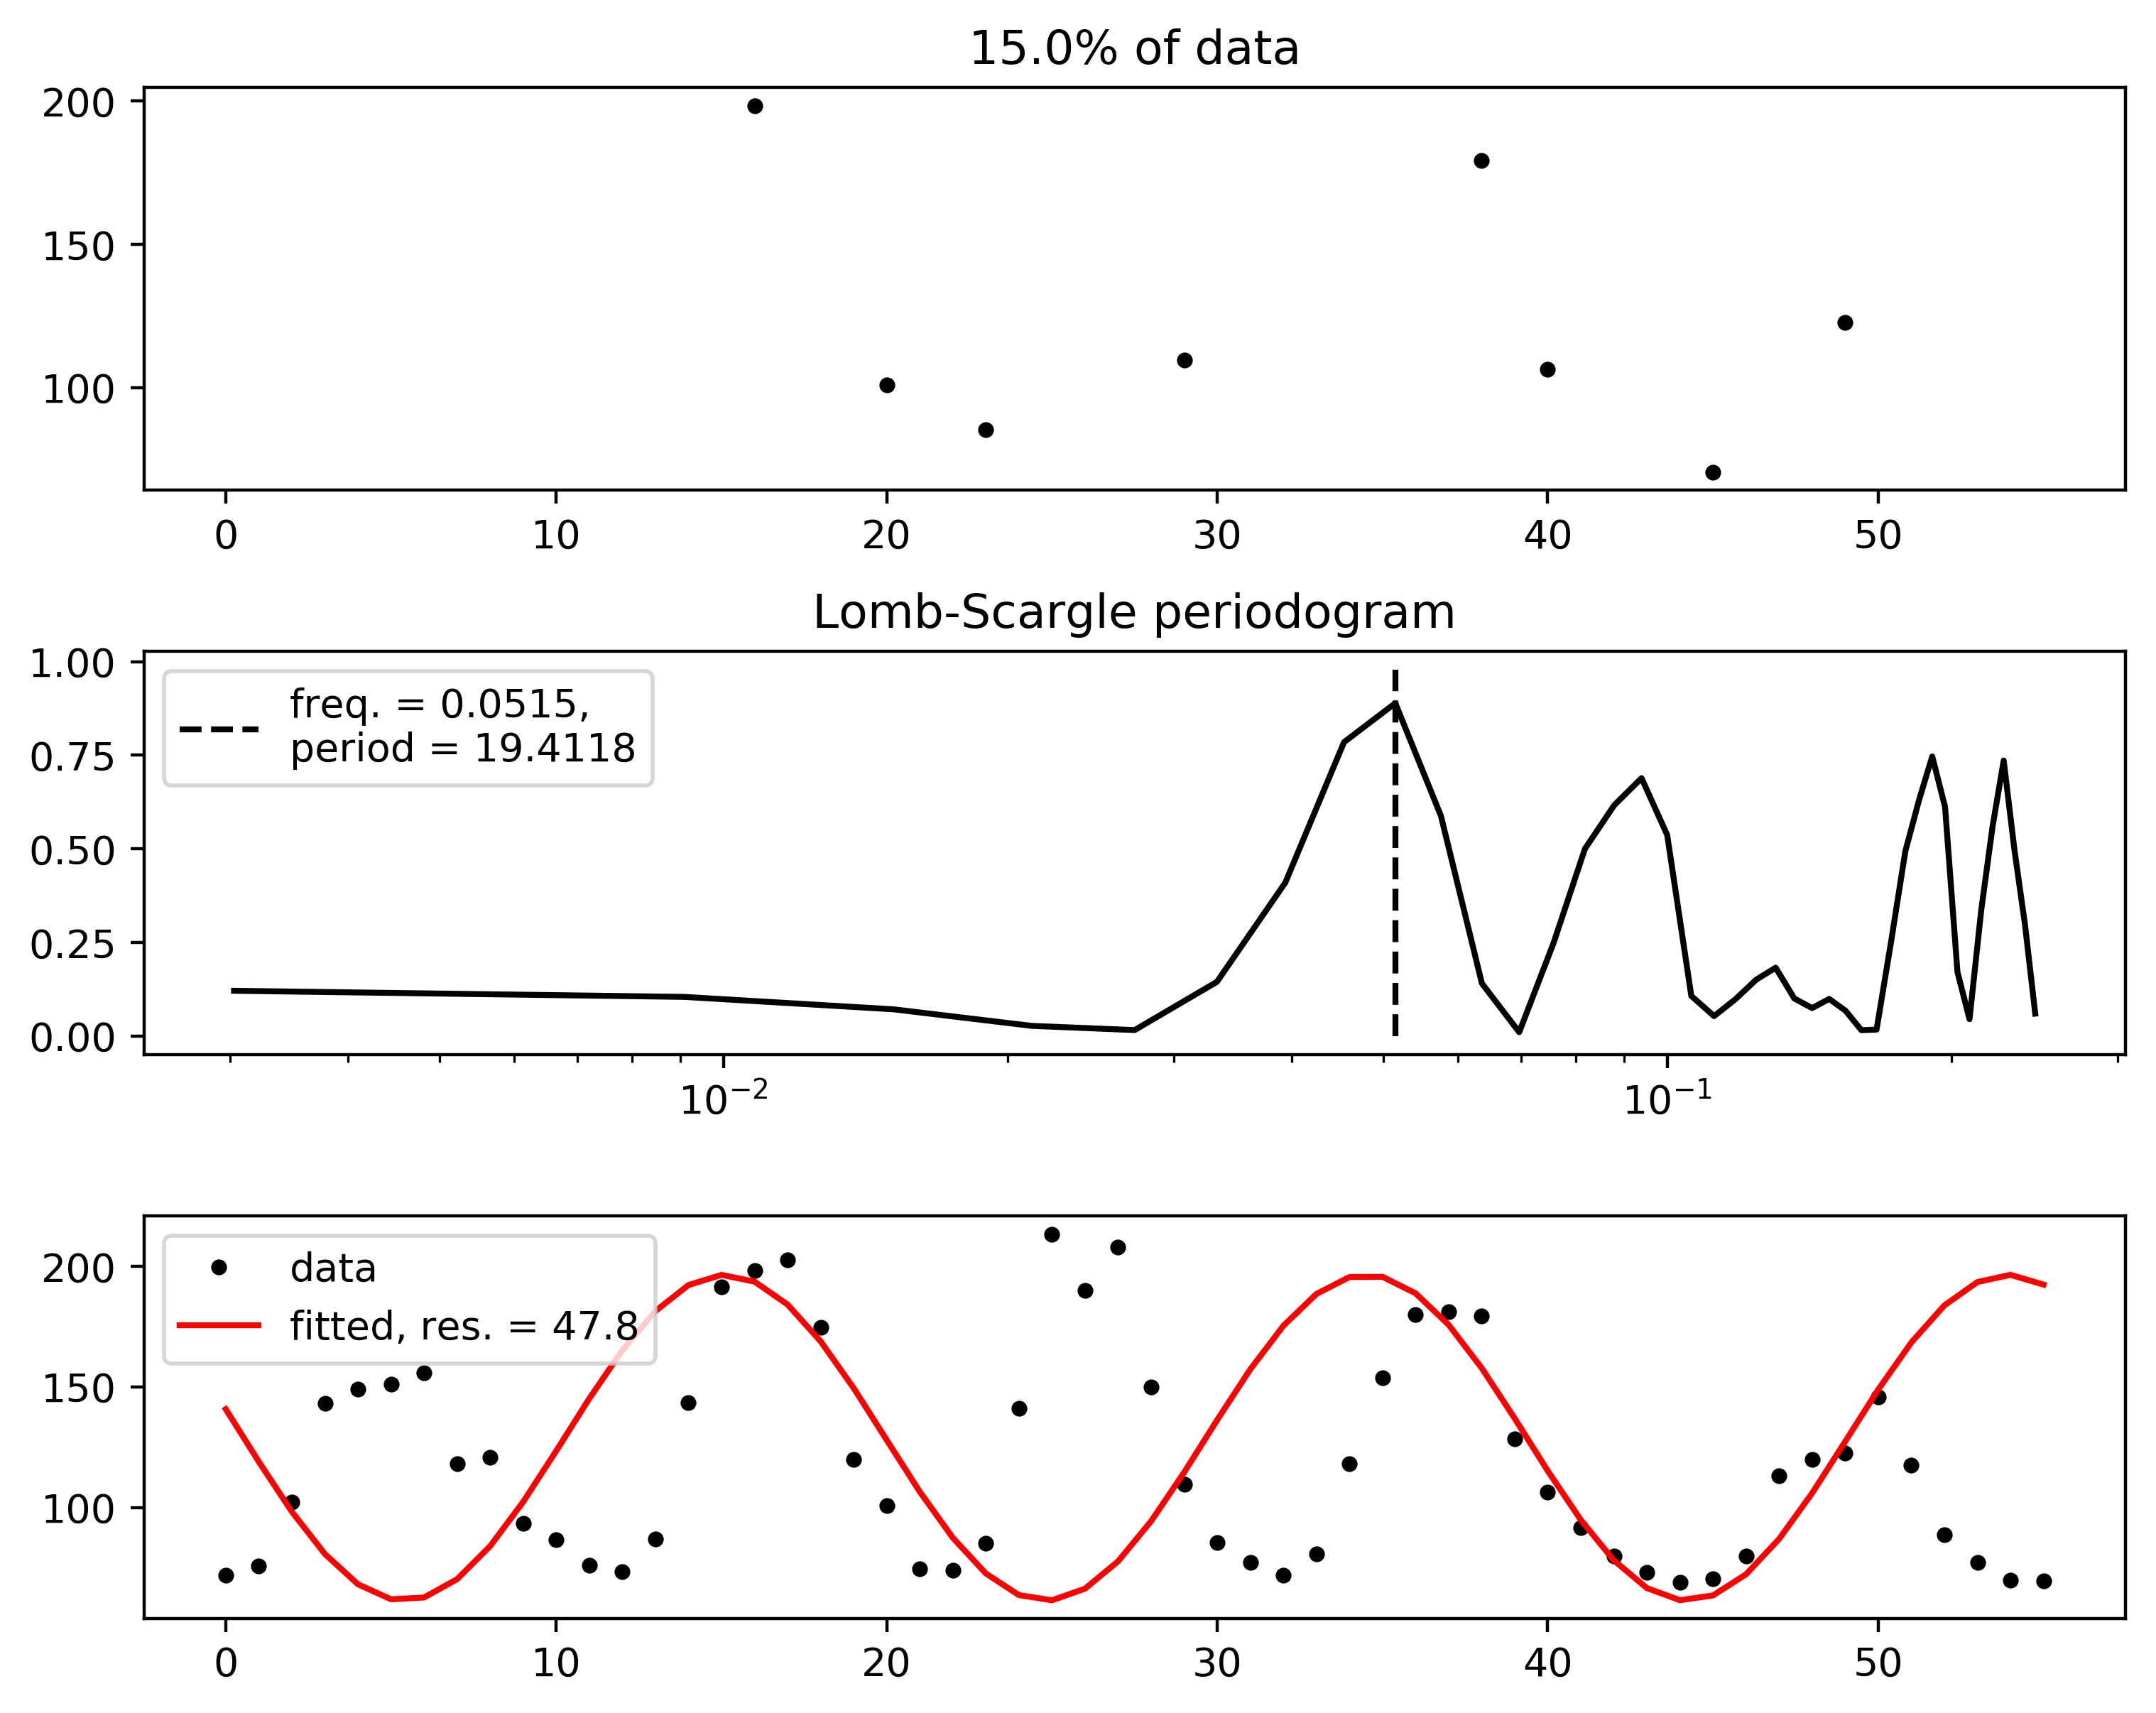
\includegraphics[scale=0.55]{../scripts/dataset3/periodograms_ny2.0_model1_pg0.85.jpg}
\end{center}
\end{frame}
\begin{frame}
\frametitle{Scenario 2 - yearly averages}
\begin{center}
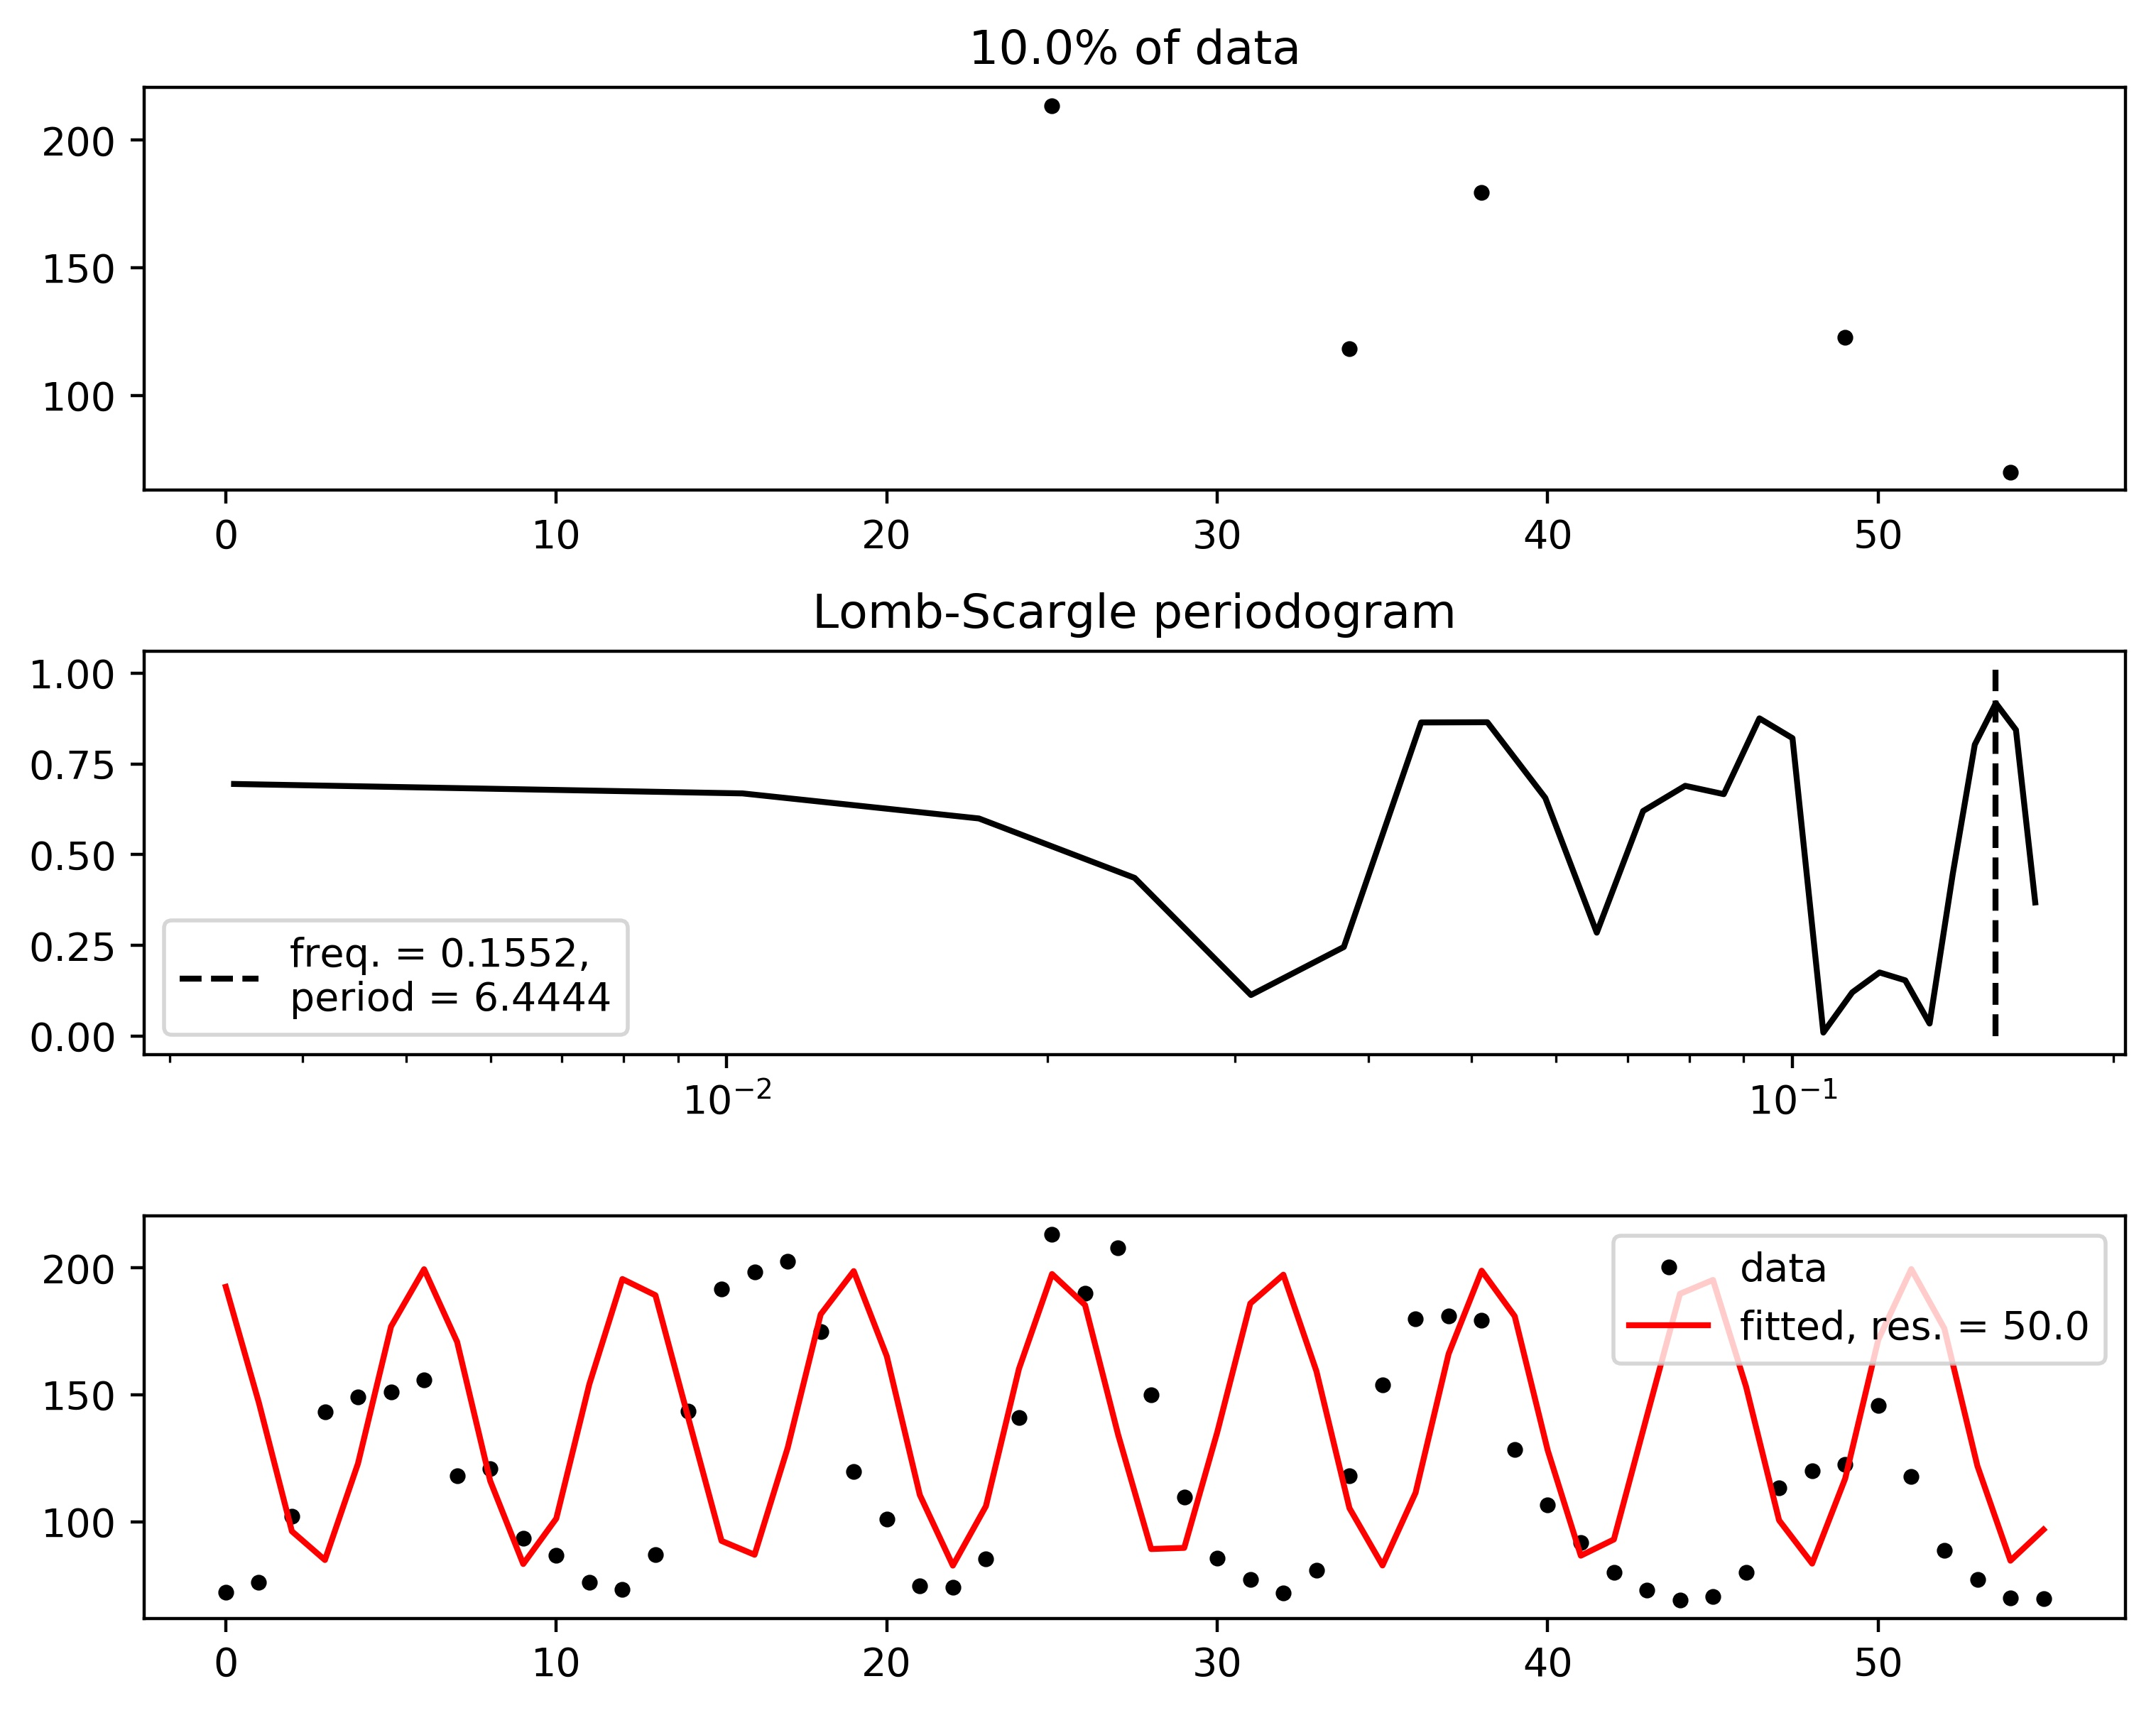
\includegraphics[scale=0.55]{../scripts/dataset3/periodograms_ny2.0_model1_pg0.9.jpg}
\end{center}
\end{frame}
\begin{frame}
\frametitle{Scenario 2 - yearly averages}
\begin{center}
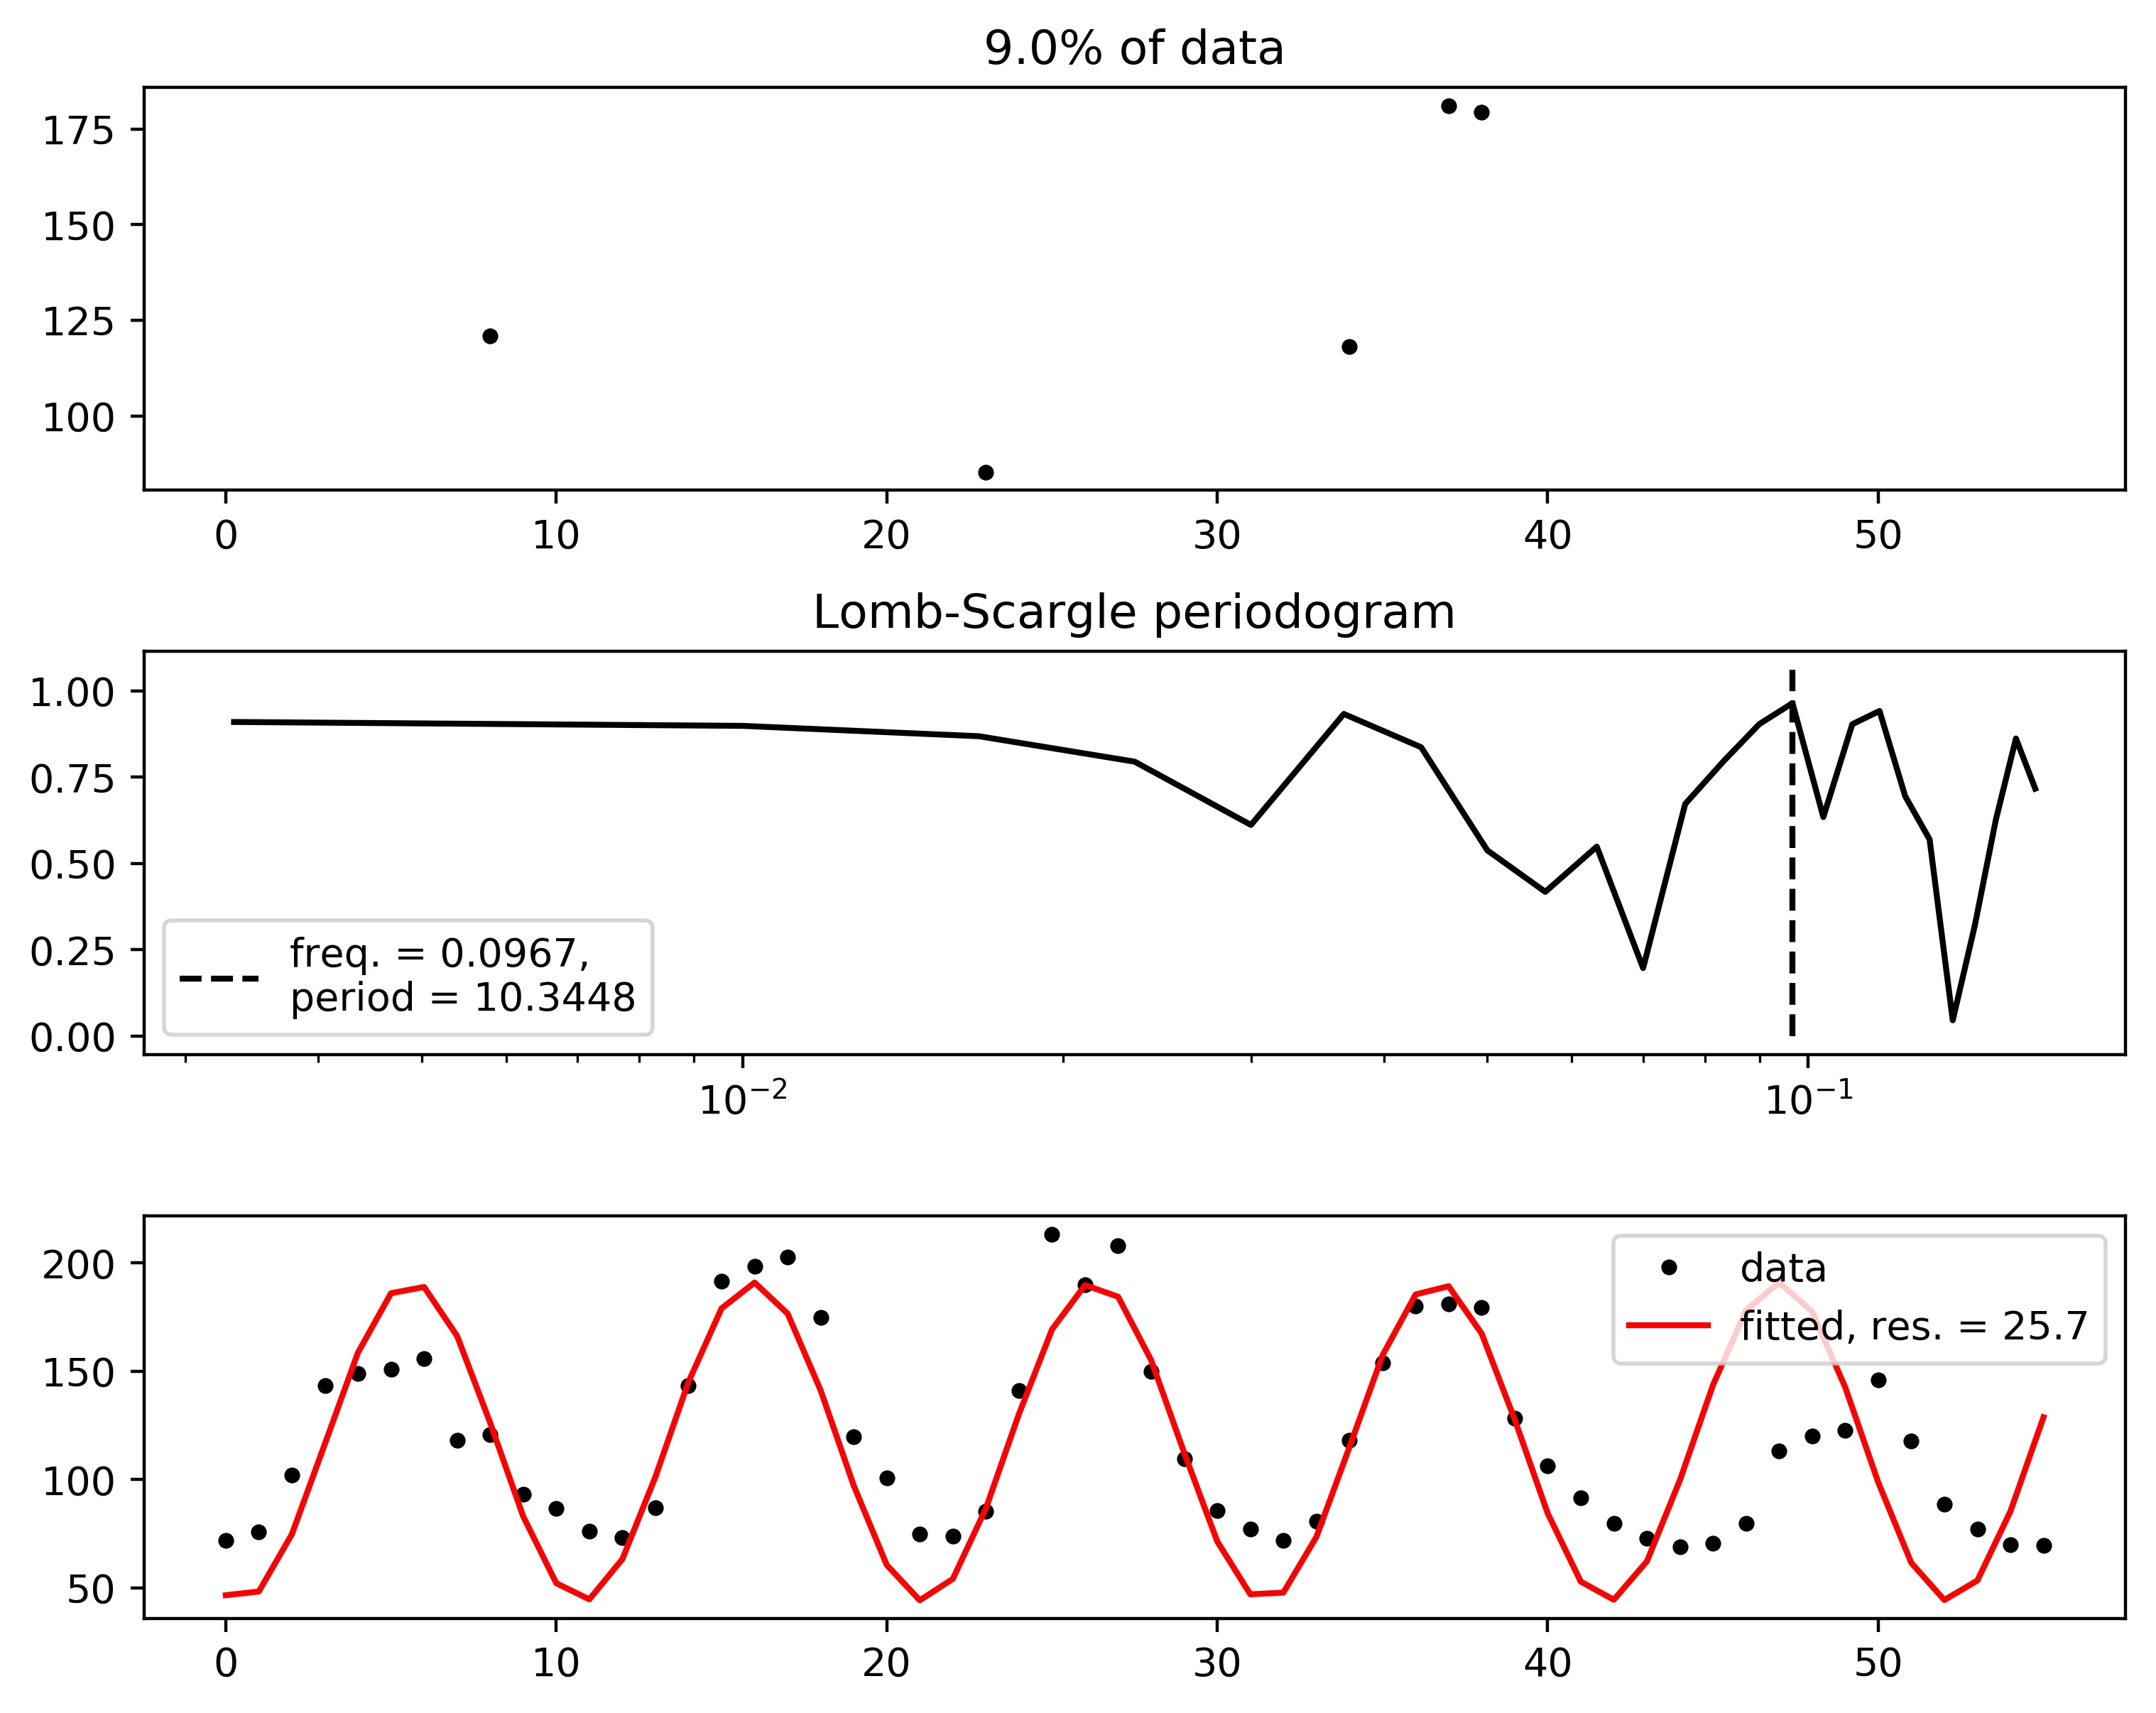
\includegraphics[scale=0.55]{../scripts/dataset3/periodograms_ny2.0_model1_pg0.91.jpg}
\end{center}
\end{frame}
\begin{frame}
\frametitle{Scenario 2 - yearly averages}
\begin{center}
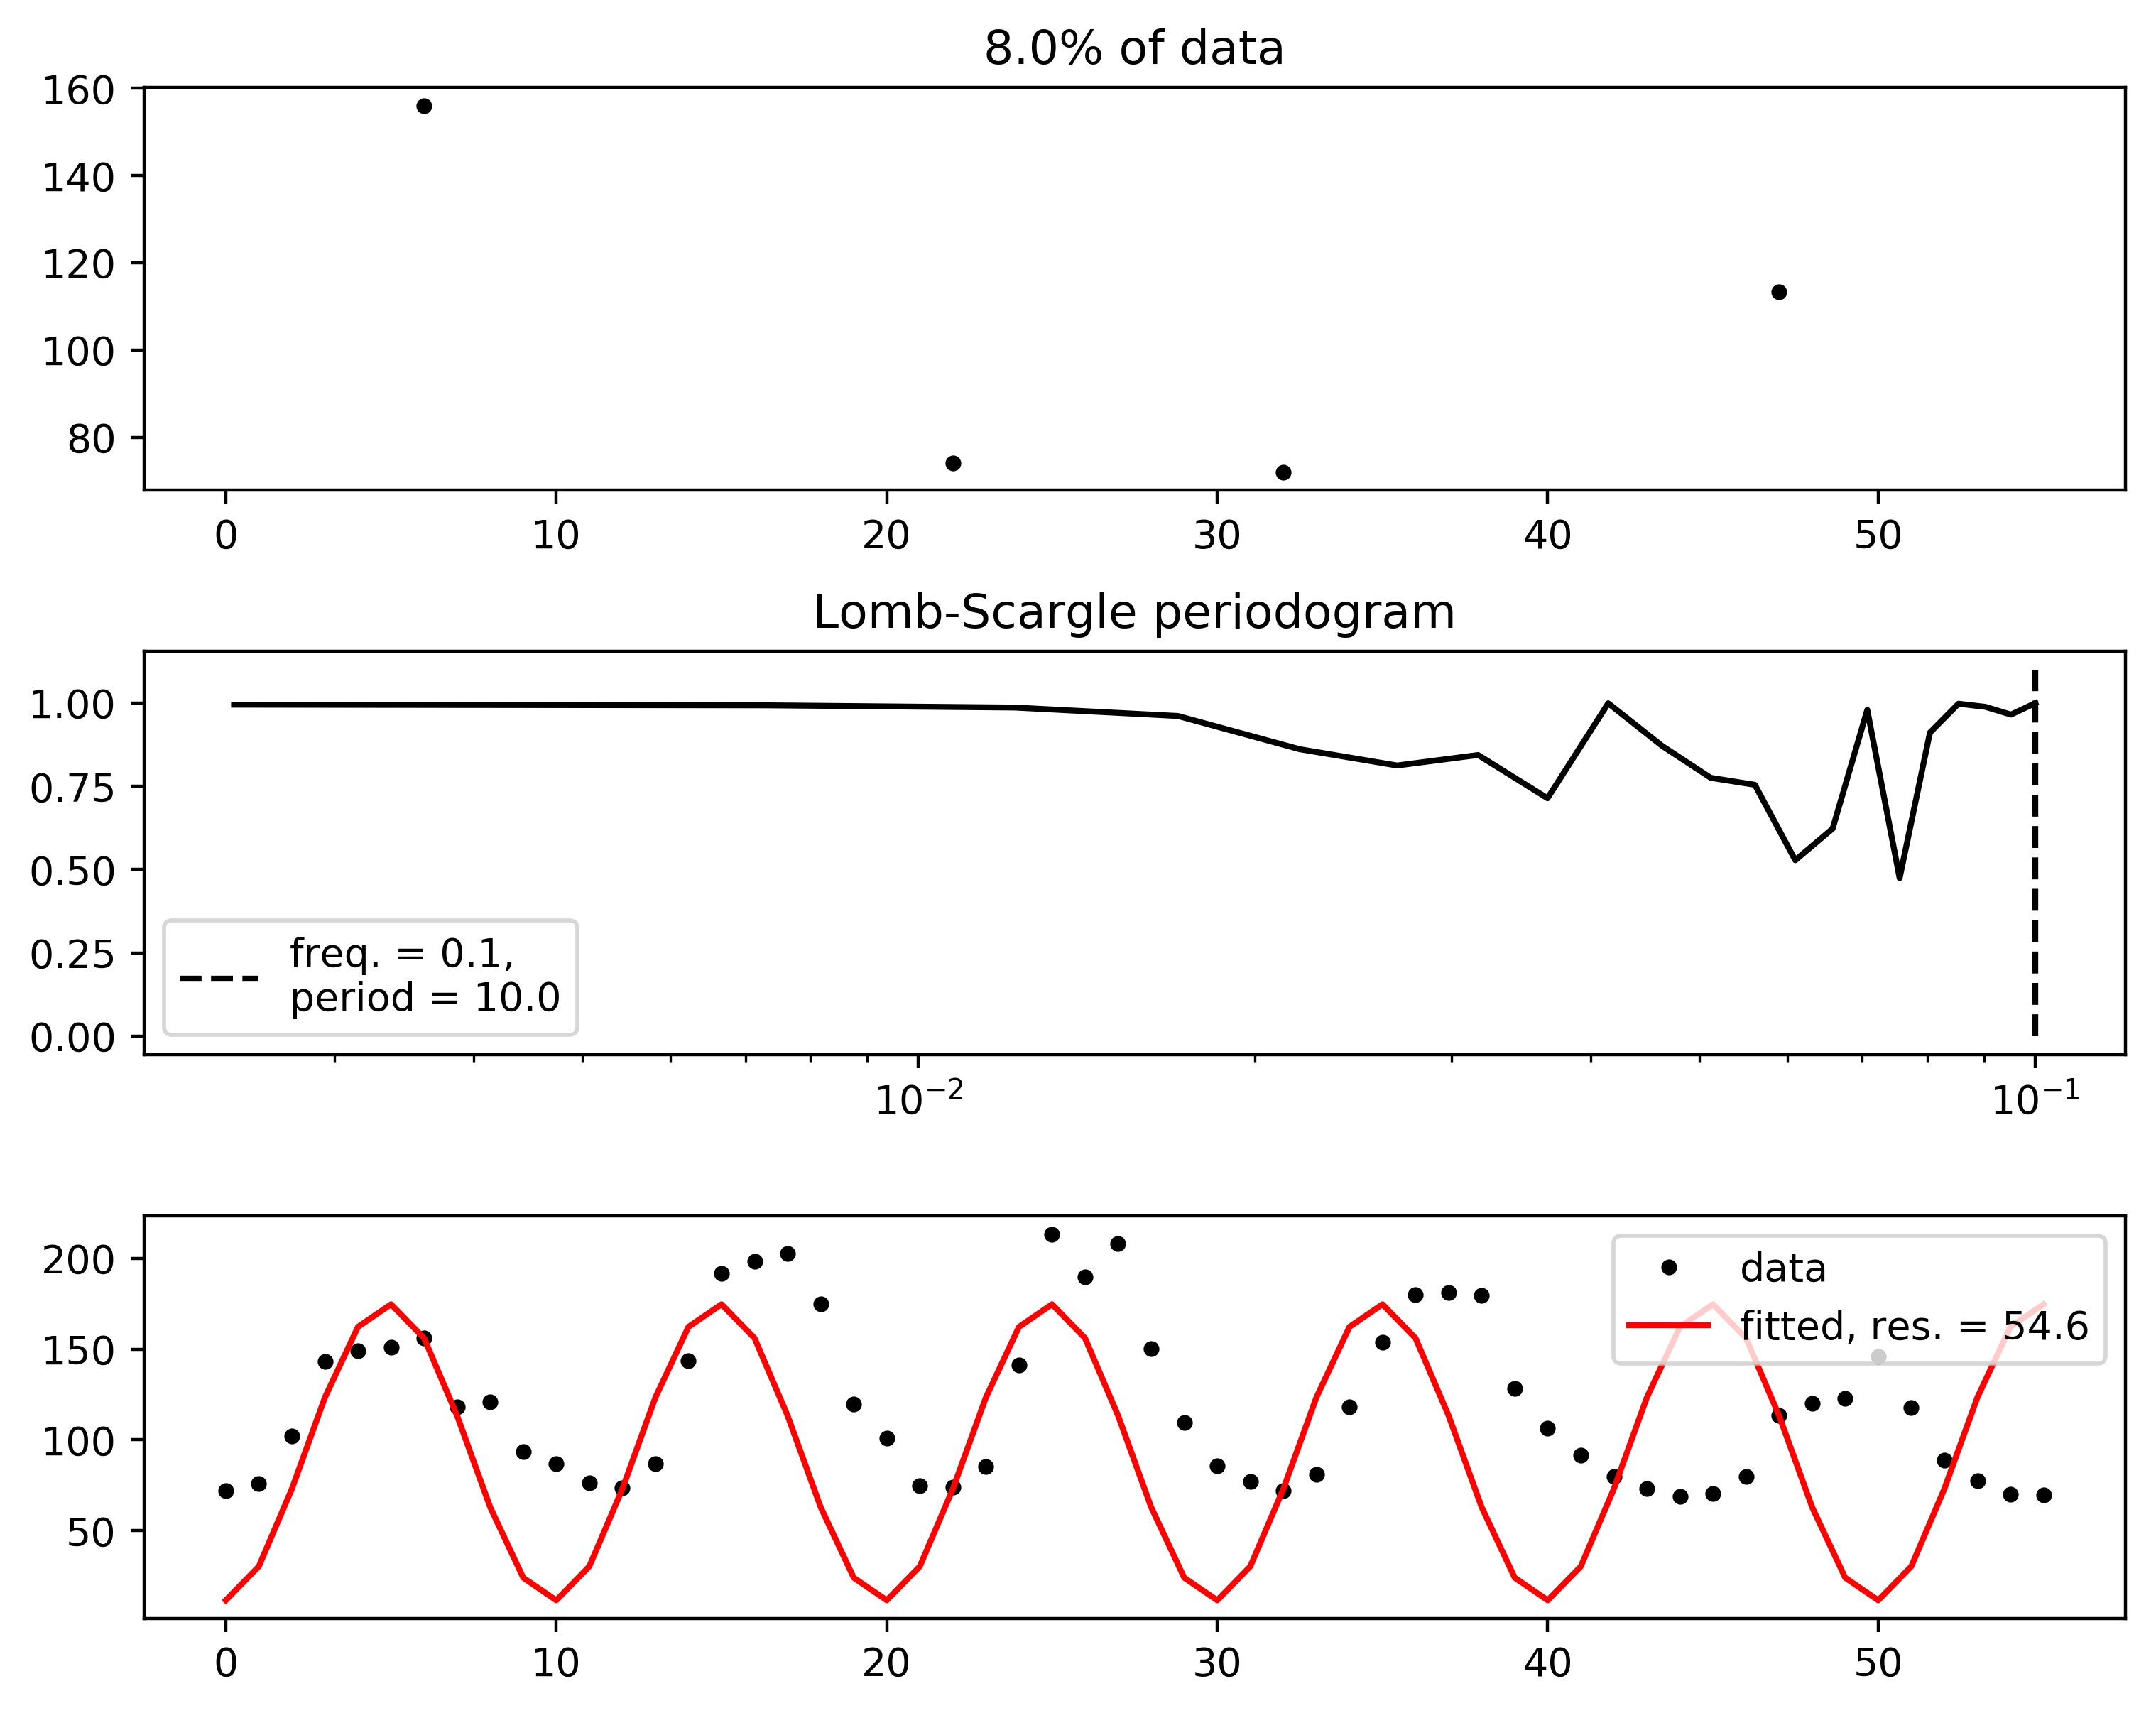
\includegraphics[scale=0.55]{../scripts/dataset3/periodograms_ny2.0_model1_pg0.92.jpg}
\end{center}
\end{frame}


\section{Final remarks}

%%%%%%%%%%%%%%%%%%%%%%%%  FRAME  %%%%%%%%%%%%%%%%%%%%%%%%
\begin{frame}
\frametitle{Final remarks}
\begin{itemize}
\item Effects of sampling discussed
\item Experiments undertaken with two scenarios of uneven sampling
\item Lomb-Scargle periodogram introduced and applied via \texttt{LombScargle} class (from \texttt{Python}'s package \texttt{astropy})
\item Parameter \texttt{nyquist\_factor} tuned during analysis
\item The tool was successfully implemented 
\end{itemize}
\end{frame}

%%%%%%%%%%%%%%%%%%%%%%%%  FRAME  %%%%%%%%%%%%%%%%%%%%%%%%
\begin{frame}
\frametitle{Links}
Source of the data: \\
\begin{center}
\href{https://omniweb.gsfc.nasa.gov/form/dx1.html}{omniweb.gsfc.nasa.gov/form/dx1.html}
\end{center}
\vspace{2mm}
Documentation of the tool (\texttt{astropy}'s \texttt{LombScargle} class): \\
\begin{center}
\href{https://docs.astropy.org/en/stable/timeseries/lombscargle.html}{docs.astropy.org/en/stable/timeseries/lombscargle.html}
\end{center}
\vspace{2mm}
This project's repository: \\
\begin{center}
\href{https://github.com/leosattler/projeto-lomb-scargle.git}{github.com/leosattler/projeto-lomb-scargle.git}
\end{center}
\vspace{10mm}
\center
Thank you!
\end{frame}

\end{document}